\documentclass[twoside]{book}

% Packages required by doxygen
\usepackage{calc}
\usepackage{doxygen}
\usepackage{graphicx}
\usepackage[utf8]{inputenc}
\usepackage{makeidx}
\usepackage{multicol}
\usepackage{multirow}
\usepackage{textcomp}
\usepackage[table]{xcolor}

% Font selection
\usepackage[T1]{fontenc}
\usepackage{mathptmx}
\usepackage[scaled=.90]{helvet}
\usepackage{courier}
\usepackage{amssymb}
\usepackage{sectsty}
\renewcommand{\familydefault}{\sfdefault}
\allsectionsfont{%
  \fontseries{bc}\selectfont%
  \color{darkgray}%
}
\renewcommand{\DoxyLabelFont}{%
  \fontseries{bc}\selectfont%
  \color{darkgray}%
}

% Page & text layout
\usepackage{geometry}
\geometry{%
  a4paper,%
  top=2.5cm,%
  bottom=2.5cm,%
  left=2.5cm,%
  right=2.5cm%
}
\tolerance=750
\hfuzz=15pt
\hbadness=750
\setlength{\emergencystretch}{15pt}
\setlength{\parindent}{0cm}
\setlength{\parskip}{0.2cm}
\makeatletter
\renewcommand{\paragraph}{%
  \@startsection{paragraph}{4}{0ex}{-1.0ex}{1.0ex}{%
    \normalfont\normalsize\bfseries\SS@parafont%
  }%
}
\renewcommand{\subparagraph}{%
  \@startsection{subparagraph}{5}{0ex}{-1.0ex}{1.0ex}{%
    \normalfont\normalsize\bfseries\SS@subparafont%
  }%
}
\makeatother

% Headers & footers
\usepackage{fancyhdr}
\pagestyle{fancyplain}
\fancyhead[LE]{\fancyplain{}{\bfseries\thepage}}
\fancyhead[CE]{\fancyplain{}{}}
\fancyhead[RE]{\fancyplain{}{\bfseries\leftmark}}
\fancyhead[LO]{\fancyplain{}{\bfseries\rightmark}}
\fancyhead[CO]{\fancyplain{}{}}
\fancyhead[RO]{\fancyplain{}{\bfseries\thepage}}
\fancyfoot[LE]{\fancyplain{}{}}
\fancyfoot[CE]{\fancyplain{}{}}
\fancyfoot[RE]{\fancyplain{}{\bfseries\scriptsize Generated on Sat Nov 21 2015 02\-:26\-:16 for Iteration3 by Doxygen }}
\fancyfoot[LO]{\fancyplain{}{\bfseries\scriptsize Generated on Sat Nov 21 2015 02\-:26\-:16 for Iteration3 by Doxygen }}
\fancyfoot[CO]{\fancyplain{}{}}
\fancyfoot[RO]{\fancyplain{}{}}
\renewcommand{\footrulewidth}{0.4pt}
\renewcommand{\chaptermark}[1]{%
  \markboth{#1}{}%
}
\renewcommand{\sectionmark}[1]{%
  \markright{\thesection\ #1}%
}

% Indices & bibliography
\usepackage{natbib}
\usepackage[titles]{tocloft}
\setcounter{tocdepth}{3}
\setcounter{secnumdepth}{5}
\makeindex

% Hyperlinks (required, but should be loaded last)
\usepackage{ifpdf}
\ifpdf
  \usepackage[pdftex,pagebackref=true]{hyperref}
\else
  \usepackage[ps2pdf,pagebackref=true]{hyperref}
\fi
\hypersetup{%
  colorlinks=true,%
  linkcolor=blue,%
  citecolor=blue,%
  unicode%
}

% Custom commands
\newcommand{\clearemptydoublepage}{%
  \newpage{\pagestyle{empty}\cleardoublepage}%
}


%===== C O N T E N T S =====

\begin{document}

% Titlepage & ToC
\hypersetup{pageanchor=false}
\pagenumbering{roman}
\begin{titlepage}
\vspace*{7cm}
\begin{center}%
{\Large Iteration3 }\\
\vspace*{1cm}
{\large Generated by Doxygen 1.8.6}\\
\vspace*{0.5cm}
{\small Sat Nov 21 2015 02:26:16}\\
\end{center}
\end{titlepage}
\clearemptydoublepage
\tableofcontents
\clearemptydoublepage
\pagenumbering{arabic}
\hypersetup{pageanchor=true}

%--- Begin generated contents ---
\chapter{My Personal Index Page}
\label{index}\hypertarget{index}{}\hypertarget{index_intro_sec}{}\section{Introduction}\label{index_intro_sec}
This is the introduction of our Iterition3.\hypertarget{index_install_sec}{}\section{Installation}\label{index_install_sec}
Please grade our I3 and have a good day!.\hypertarget{index_step1}{}\subsection{Step 1\-: Opening the box}\label{index_step1}
I don't know how to explain details. 
\chapter{Hierarchical Index}
\section{Class Hierarchy}
This inheritance list is sorted roughly, but not completely, alphabetically\-:\begin{DoxyCompactList}
\item \contentsline{section}{Ext\-Token}{\pageref{classExtToken}}{}
\begin{DoxyCompactList}
\item \contentsline{section}{Char\-Const\-Token}{\pageref{classCharConstToken}}{}
\item \contentsline{section}{Dash\-Token}{\pageref{classDashToken}}{}
\item \contentsline{section}{End\-Of\-File\-Token}{\pageref{classEndOfFileToken}}{}
\item \contentsline{section}{False\-Kwd\-Token}{\pageref{classFalseKwdToken}}{}
\item \contentsline{section}{Float\-Const\-Token}{\pageref{classFloatConstToken}}{}
\item \contentsline{section}{Forward\-Slash\-Token}{\pageref{classForwardSlashToken}}{}
\item \contentsline{section}{If\-Token}{\pageref{classIfToken}}{}
\item \contentsline{section}{Int\-Const\-Token}{\pageref{classIntConstToken}}{}
\item \contentsline{section}{Left\-Paren\-Token}{\pageref{classLeftParenToken}}{}
\item \contentsline{section}{Let\-Token}{\pageref{classLetToken}}{}
\item \contentsline{section}{Not\-Op\-Token}{\pageref{classNotOpToken}}{}
\item \contentsline{section}{Plus\-Sign\-Token}{\pageref{classPlusSignToken}}{}
\item \contentsline{section}{Relational\-Op\-Token}{\pageref{classRelationalOpToken}}{}
\item \contentsline{section}{Star\-Token}{\pageref{classStarToken}}{}
\item \contentsline{section}{String\-Const\-Token}{\pageref{classStringConstToken}}{}
\item \contentsline{section}{True\-Kwd\-Token}{\pageref{classTrueKwdToken}}{}
\item \contentsline{section}{Variable\-Name\-Token}{\pageref{classVariableNameToken}}{}
\end{DoxyCompactList}
\item \contentsline{section}{Node}{\pageref{classNode}}{}
\begin{DoxyCompactList}
\item \contentsline{section}{Decl}{\pageref{classDecl}}{}
\begin{DoxyCompactList}
\item \contentsline{section}{Extended\-Matrix\-Decl}{\pageref{classExtendedMatrixDecl}}{}
\item \contentsline{section}{Kwd\-Decl}{\pageref{classKwdDecl}}{}
\item \contentsline{section}{Matrix\-Decl}{\pageref{classMatrixDecl}}{}
\end{DoxyCompactList}
\item \contentsline{section}{Expr}{\pageref{classExpr}}{}
\begin{DoxyCompactList}
\item \contentsline{section}{Any\-Expr}{\pageref{classAnyExpr}}{}
\item \contentsline{section}{Bin\-Op\-Expr}{\pageref{classBinOpExpr}}{}
\item \contentsline{section}{Boolean\-Expr}{\pageref{classBooleanExpr}}{}
\item \contentsline{section}{If\-Else\-Expr}{\pageref{classIfElseExpr}}{}
\item \contentsline{section}{Let\-Expr}{\pageref{classLetExpr}}{}
\item \contentsline{section}{Matrix\-Ref\-Expr}{\pageref{classMatrixRefExpr}}{}
\item \contentsline{section}{Nested\-Expr}{\pageref{classNestedExpr}}{}
\item \contentsline{section}{Nested\-Or\-Function\-Call\-Expr}{\pageref{classNestedOrFunctionCallExpr}}{}
\item \contentsline{section}{Not\-Expr}{\pageref{classNotExpr}}{}
\item \contentsline{section}{Var\-Expr}{\pageref{classVarExpr}}{}
\end{DoxyCompactList}
\item \contentsline{section}{Program}{\pageref{classProgram}}{}
\item \contentsline{section}{Stmt}{\pageref{classStmt}}{}
\begin{DoxyCompactList}
\item \contentsline{section}{Assign\-Stmt}{\pageref{classAssignStmt}}{}
\item \contentsline{section}{Extended\-Assign\-Stmt}{\pageref{classExtendedAssignStmt}}{}
\item \contentsline{section}{If\-Else\-Stmt}{\pageref{classIfElseStmt}}{}
\item \contentsline{section}{If\-Stmt}{\pageref{classIfStmt}}{}
\item \contentsline{section}{Print\-Stmt}{\pageref{classPrintStmt}}{}
\item \contentsline{section}{Repeat\-Stmt}{\pageref{classRepeatStmt}}{}
\item \contentsline{section}{Stmt\-Decl}{\pageref{classStmtDecl}}{}
\item \contentsline{section}{Stmts\-Stmt}{\pageref{classStmtsStmt}}{}
\item \contentsline{section}{While\-Stmt}{\pageref{classWhileStmt}}{}
\end{DoxyCompactList}
\item \contentsline{section}{Stmts}{\pageref{classStmts}}{}
\begin{DoxyCompactList}
\item \contentsline{section}{Empty\-Stmts}{\pageref{classEmptyStmts}}{}
\item \contentsline{section}{Stmts\-Seq}{\pageref{classStmtsSeq}}{}
\end{DoxyCompactList}
\end{DoxyCompactList}
\item \contentsline{section}{Parser}{\pageref{classParser}}{}
\item \contentsline{section}{Parse\-Result}{\pageref{classParseResult}}{}
\item \contentsline{section}{Scanner}{\pageref{classScanner}}{}
\item Test\-Suite\begin{DoxyCompactList}
\item \contentsline{section}{Ast\-Test\-Suite}{\pageref{classAstTestSuite}}{}
\item \contentsline{section}{Parser\-Test\-Suite}{\pageref{classParserTestSuite}}{}
\item \contentsline{section}{Regex\-Test\-Suite}{\pageref{classRegexTestSuite}}{}
\item \contentsline{section}{Scanner\-Test\-Suite}{\pageref{classScannerTestSuite}}{}
\end{DoxyCompactList}
\item \contentsline{section}{Token}{\pageref{classToken}}{}
\end{DoxyCompactList}

\chapter{Class Index}
\section{Class List}
Here are the classes, structs, unions and interfaces with brief descriptions\-:\begin{DoxyCompactList}
\item\contentsline{section}{\hyperlink{classAnyExpr}{Any\-Expr} }{\pageref{classAnyExpr}}{}
\item\contentsline{section}{\hyperlink{classAssignStmt}{Assign\-Stmt} }{\pageref{classAssignStmt}}{}
\item\contentsline{section}{\hyperlink{classAstTestSuite}{Ast\-Test\-Suite} }{\pageref{classAstTestSuite}}{}
\item\contentsline{section}{\hyperlink{classBinOpExpr}{Bin\-Op\-Expr} }{\pageref{classBinOpExpr}}{}
\item\contentsline{section}{\hyperlink{classBooleanExpr}{Boolean\-Expr} }{\pageref{classBooleanExpr}}{}
\item\contentsline{section}{\hyperlink{classCharConstToken}{Char\-Const\-Token} }{\pageref{classCharConstToken}}{}
\item\contentsline{section}{\hyperlink{classDashToken}{Dash\-Token} }{\pageref{classDashToken}}{}
\item\contentsline{section}{\hyperlink{classDecl}{Decl} }{\pageref{classDecl}}{}
\item\contentsline{section}{\hyperlink{classEmptyStmts}{Empty\-Stmts} }{\pageref{classEmptyStmts}}{}
\item\contentsline{section}{\hyperlink{classEndOfFileToken}{End\-Of\-File\-Token} }{\pageref{classEndOfFileToken}}{}
\item\contentsline{section}{\hyperlink{classExpr}{Expr} }{\pageref{classExpr}}{}
\item\contentsline{section}{\hyperlink{classExtendedAssignStmt}{Extended\-Assign\-Stmt} }{\pageref{classExtendedAssignStmt}}{}
\item\contentsline{section}{\hyperlink{classExtendedMatrixDecl}{Extended\-Matrix\-Decl} }{\pageref{classExtendedMatrixDecl}}{}
\item\contentsline{section}{\hyperlink{classExtToken}{Ext\-Token} }{\pageref{classExtToken}}{}
\item\contentsline{section}{\hyperlink{classFalseKwdToken}{False\-Kwd\-Token} }{\pageref{classFalseKwdToken}}{}
\item\contentsline{section}{\hyperlink{classFloatConstToken}{Float\-Const\-Token} }{\pageref{classFloatConstToken}}{}
\item\contentsline{section}{\hyperlink{classForwardSlashToken}{Forward\-Slash\-Token} }{\pageref{classForwardSlashToken}}{}
\item\contentsline{section}{\hyperlink{classIfElseExpr}{If\-Else\-Expr} }{\pageref{classIfElseExpr}}{}
\item\contentsline{section}{\hyperlink{classIfElseStmt}{If\-Else\-Stmt} }{\pageref{classIfElseStmt}}{}
\item\contentsline{section}{\hyperlink{classIfStmt}{If\-Stmt} }{\pageref{classIfStmt}}{}
\item\contentsline{section}{\hyperlink{classIfToken}{If\-Token} }{\pageref{classIfToken}}{}
\item\contentsline{section}{\hyperlink{classIntConstToken}{Int\-Const\-Token} }{\pageref{classIntConstToken}}{}
\item\contentsline{section}{\hyperlink{classKwdDecl}{Kwd\-Decl} }{\pageref{classKwdDecl}}{}
\item\contentsline{section}{\hyperlink{classLeftParenToken}{Left\-Paren\-Token} }{\pageref{classLeftParenToken}}{}
\item\contentsline{section}{\hyperlink{classLetExpr}{Let\-Expr} }{\pageref{classLetExpr}}{}
\item\contentsline{section}{\hyperlink{classLetToken}{Let\-Token} }{\pageref{classLetToken}}{}
\item\contentsline{section}{\hyperlink{classMatrixDecl}{Matrix\-Decl} }{\pageref{classMatrixDecl}}{}
\item\contentsline{section}{\hyperlink{classMatrixRefExpr}{Matrix\-Ref\-Expr} }{\pageref{classMatrixRefExpr}}{}
\item\contentsline{section}{\hyperlink{classNestedExpr}{Nested\-Expr} }{\pageref{classNestedExpr}}{}
\item\contentsline{section}{\hyperlink{classNestedOrFunctionCallExpr}{Nested\-Or\-Function\-Call\-Expr} }{\pageref{classNestedOrFunctionCallExpr}}{}
\item\contentsline{section}{\hyperlink{classNode}{Node} }{\pageref{classNode}}{}
\item\contentsline{section}{\hyperlink{classNotExpr}{Not\-Expr} }{\pageref{classNotExpr}}{}
\item\contentsline{section}{\hyperlink{classNotOpToken}{Not\-Op\-Token} }{\pageref{classNotOpToken}}{}
\item\contentsline{section}{\hyperlink{classParser}{Parser} }{\pageref{classParser}}{}
\item\contentsline{section}{\hyperlink{classParseResult}{Parse\-Result} }{\pageref{classParseResult}}{}
\item\contentsline{section}{\hyperlink{classParserTestSuite}{Parser\-Test\-Suite} }{\pageref{classParserTestSuite}}{}
\item\contentsline{section}{\hyperlink{classPlusSignToken}{Plus\-Sign\-Token} }{\pageref{classPlusSignToken}}{}
\item\contentsline{section}{\hyperlink{classPrintStmt}{Print\-Stmt} }{\pageref{classPrintStmt}}{}
\item\contentsline{section}{\hyperlink{classProgram}{Program} }{\pageref{classProgram}}{}
\item\contentsline{section}{\hyperlink{classRegexTestSuite}{Regex\-Test\-Suite} }{\pageref{classRegexTestSuite}}{}
\item\contentsline{section}{\hyperlink{classRelationalOpToken}{Relational\-Op\-Token} }{\pageref{classRelationalOpToken}}{}
\item\contentsline{section}{\hyperlink{classRepeatStmt}{Repeat\-Stmt} }{\pageref{classRepeatStmt}}{}
\item\contentsline{section}{\hyperlink{classScanner}{Scanner} }{\pageref{classScanner}}{}
\item\contentsline{section}{\hyperlink{classScannerTestSuite}{Scanner\-Test\-Suite} }{\pageref{classScannerTestSuite}}{}
\item\contentsline{section}{\hyperlink{classStarToken}{Star\-Token} }{\pageref{classStarToken}}{}
\item\contentsline{section}{\hyperlink{classStmt}{Stmt} }{\pageref{classStmt}}{}
\item\contentsline{section}{\hyperlink{classStmtDecl}{Stmt\-Decl} }{\pageref{classStmtDecl}}{}
\item\contentsline{section}{\hyperlink{classStmts}{Stmts} }{\pageref{classStmts}}{}
\item\contentsline{section}{\hyperlink{classStmtsSeq}{Stmts\-Seq} }{\pageref{classStmtsSeq}}{}
\item\contentsline{section}{\hyperlink{classStmtsStmt}{Stmts\-Stmt} }{\pageref{classStmtsStmt}}{}
\item\contentsline{section}{\hyperlink{classStringConstToken}{String\-Const\-Token} }{\pageref{classStringConstToken}}{}
\item\contentsline{section}{\hyperlink{classToken}{Token} }{\pageref{classToken}}{}
\item\contentsline{section}{\hyperlink{classTrueKwdToken}{True\-Kwd\-Token} }{\pageref{classTrueKwdToken}}{}
\item\contentsline{section}{\hyperlink{classVarExpr}{Var\-Expr} }{\pageref{classVarExpr}}{}
\item\contentsline{section}{\hyperlink{classVariableNameToken}{Variable\-Name\-Token} }{\pageref{classVariableNameToken}}{}
\item\contentsline{section}{\hyperlink{classWhileStmt}{While\-Stmt} }{\pageref{classWhileStmt}}{}
\end{DoxyCompactList}

\chapter{Class Documentation}
\hypertarget{classAnyExpr}{\section{Any\-Expr Class Reference}
\label{classAnyExpr}\index{Any\-Expr@{Any\-Expr}}
}
Inheritance diagram for Any\-Expr\-:\begin{figure}[H]
\begin{center}
\leavevmode
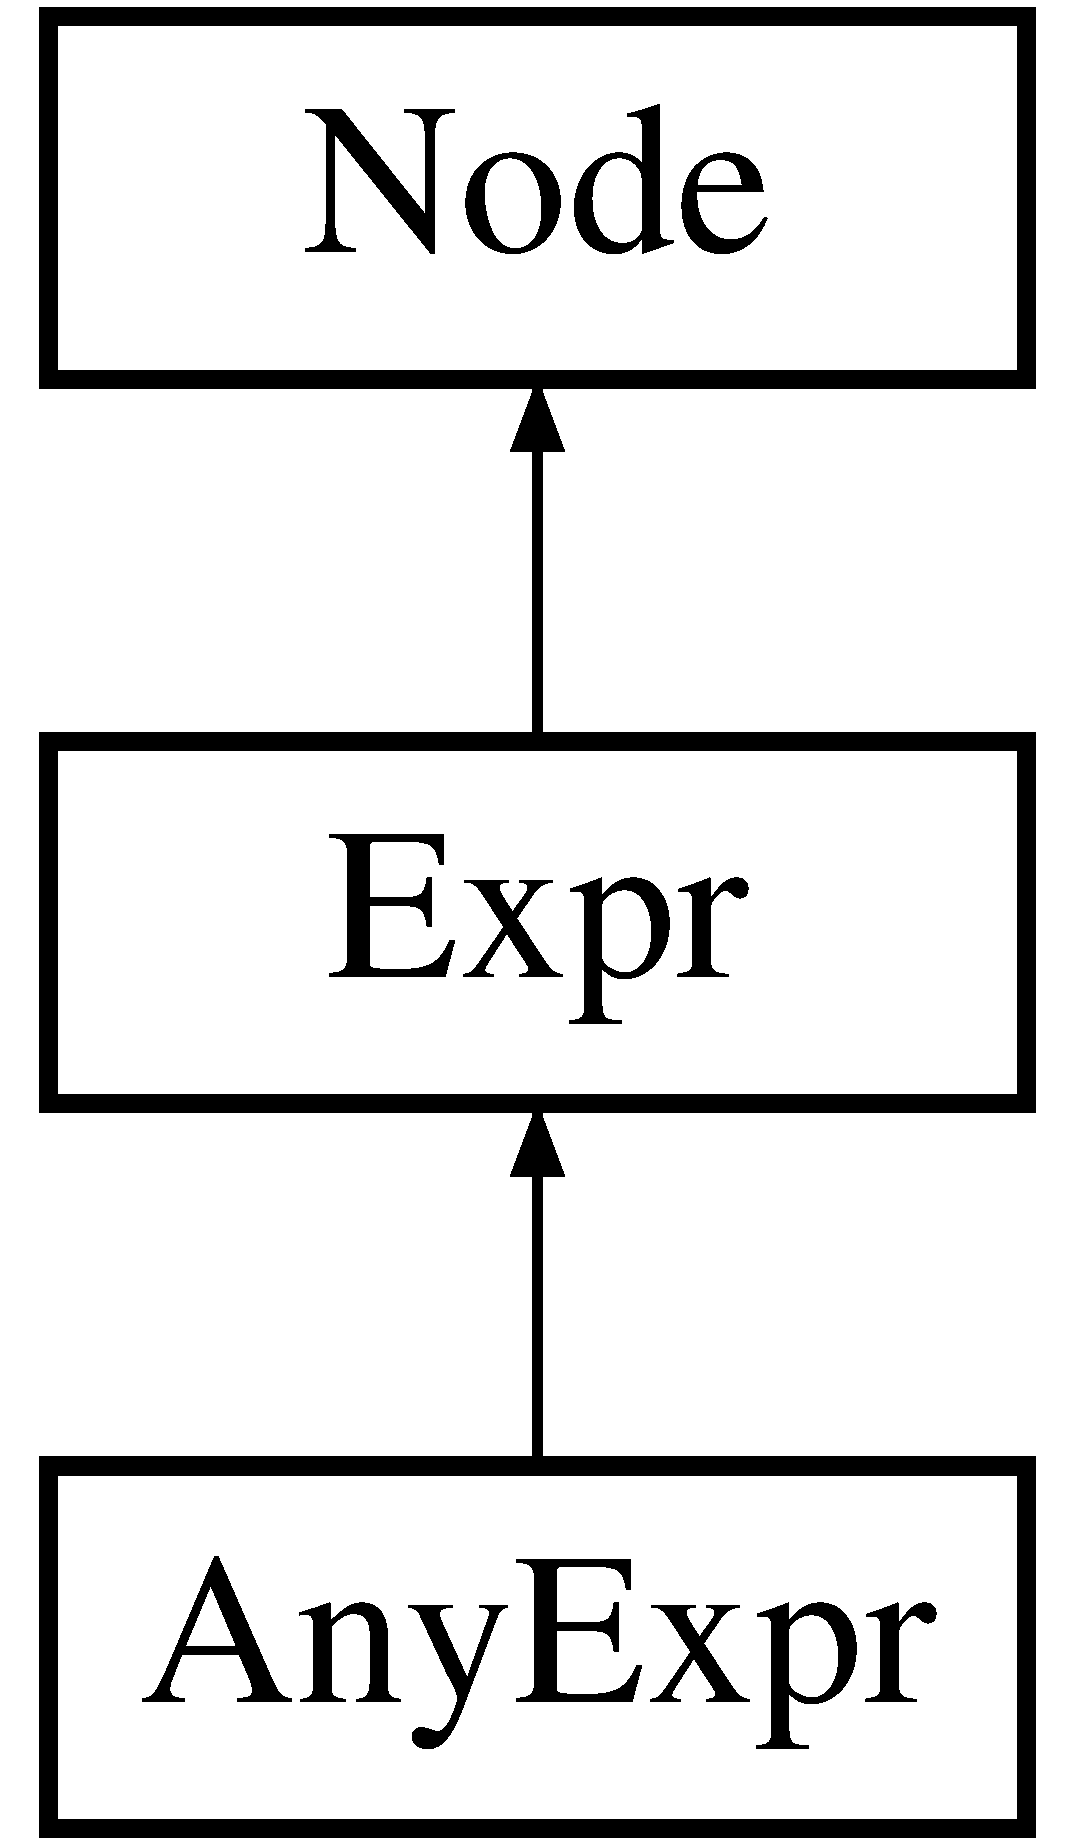
\includegraphics[height=3.000000cm]{classAnyExpr}
\end{center}
\end{figure}
\subsection*{Public Member Functions}
\begin{DoxyCompactItemize}
\item 
\hypertarget{classAnyExpr_a32bb417b464c1971ae3f8f07c9bb8e83}{\hyperlink{classAnyExpr_a32bb417b464c1971ae3f8f07c9bb8e83}{Any\-Expr} (std\-::string \-\_\-any\-Str)}\label{classAnyExpr_a32bb417b464c1971ae3f8f07c9bb8e83}

\begin{DoxyCompactList}\small\item\em Constructor for Const\-Expr node. \end{DoxyCompactList}\item 
\hypertarget{classAnyExpr_aa0dbd30150aca87996a4ed7ab18b3a8e}{std\-::string \hyperlink{classAnyExpr_aa0dbd30150aca87996a4ed7ab18b3a8e}{unparse} ()}\label{classAnyExpr_aa0dbd30150aca87996a4ed7ab18b3a8e}

\begin{DoxyCompactList}\small\item\em integer\-Const $\vert$ float\-Const $\vert$ string\-Const \end{DoxyCompactList}\end{DoxyCompactItemize}


The documentation for this class was generated from the following files\-:\begin{DoxyCompactItemize}
\item 
A\-S\-T.\-h\item 
A\-S\-T.\-cpp\end{DoxyCompactItemize}

\hypertarget{classAssignStmt}{\section{Assign\-Stmt Class Reference}
\label{classAssignStmt}\index{Assign\-Stmt@{Assign\-Stmt}}
}
Inheritance diagram for Assign\-Stmt\-:\begin{figure}[H]
\begin{center}
\leavevmode
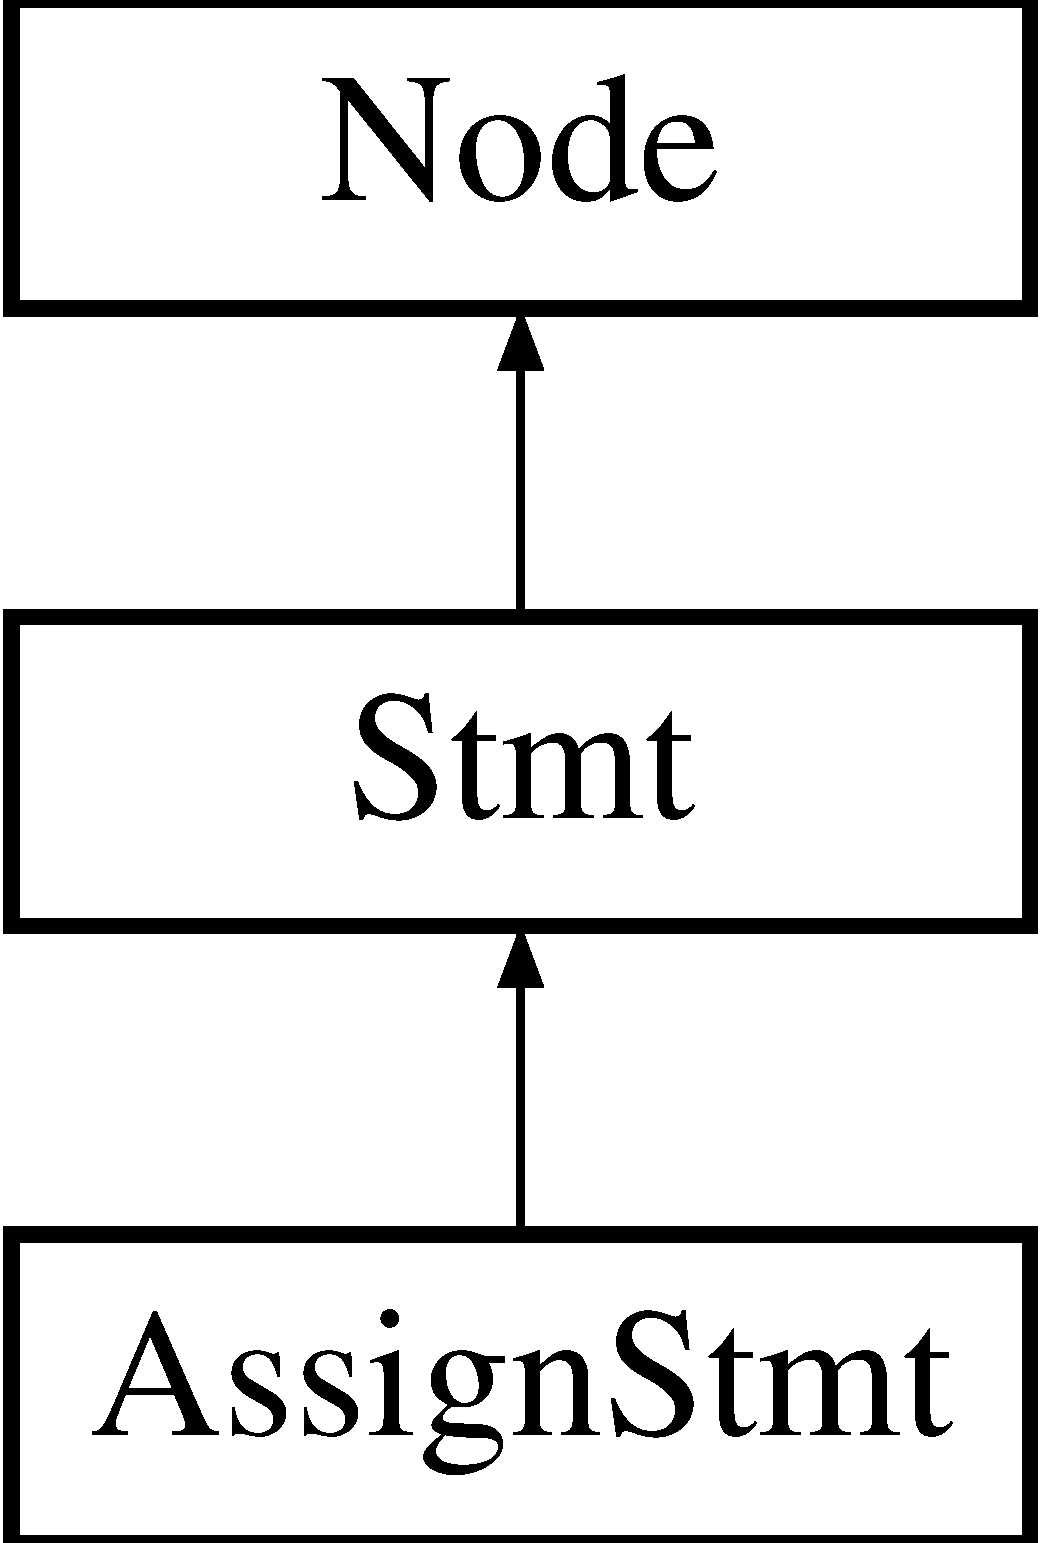
\includegraphics[height=3.000000cm]{classAssignStmt}
\end{center}
\end{figure}
\subsection*{Public Member Functions}
\begin{DoxyCompactItemize}
\item 
\hypertarget{classAssignStmt_a97d349414b5b4f701d3b100b809ab87b}{\hyperlink{classAssignStmt_a97d349414b5b4f701d3b100b809ab87b}{Assign\-Stmt} (std\-::string \-\_\-varname, \hyperlink{classExpr}{Expr} $\ast$\-\_\-expr)}\label{classAssignStmt_a97d349414b5b4f701d3b100b809ab87b}

\begin{DoxyCompactList}\small\item\em Constructor for \hyperlink{classAssignStmt}{Assign\-Stmt} node. \end{DoxyCompactList}\item 
\hypertarget{classAssignStmt_a75c486b76cc79311bfb5348175b769e2}{std\-::string \hyperlink{classAssignStmt_a75c486b76cc79311bfb5348175b769e2}{unparse} ()}\label{classAssignStmt_a75c486b76cc79311bfb5348175b769e2}

\begin{DoxyCompactList}\small\item\em var\-Name '=' \hyperlink{classExpr}{Expr} ';' \end{DoxyCompactList}\end{DoxyCompactItemize}


The documentation for this class was generated from the following files\-:\begin{DoxyCompactItemize}
\item 
A\-S\-T.\-h\item 
A\-S\-T.\-cpp\end{DoxyCompactItemize}

\hypertarget{classAstTestSuite}{\section{Ast\-Test\-Suite Class Reference}
\label{classAstTestSuite}\index{Ast\-Test\-Suite@{Ast\-Test\-Suite}}
}
Inheritance diagram for Ast\-Test\-Suite\-:\begin{figure}[H]
\begin{center}
\leavevmode
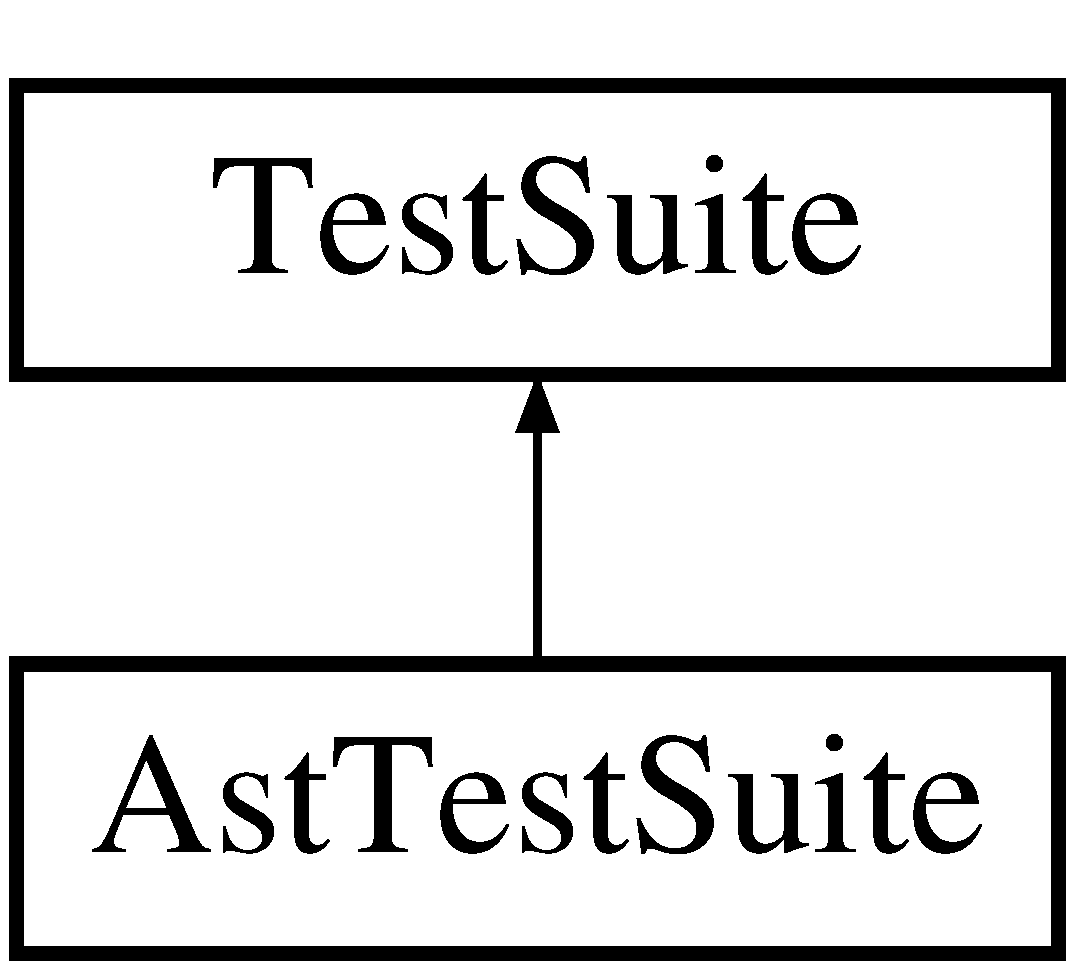
\includegraphics[height=2.000000cm]{classAstTestSuite}
\end{center}
\end{figure}
\subsection*{Public Member Functions}
\begin{DoxyCompactItemize}
\item 
\hypertarget{classAstTestSuite_a2f0462e7a965acda10e09e70432cab40}{char $\ast$$\ast$ {\bfseries make\-Args} (const char $\ast$a0, const char $\ast$a1)}\label{classAstTestSuite_a2f0462e7a965acda10e09e70432cab40}

\item 
\hypertarget{classAstTestSuite_ab935b3c95647b24b5f250b7e3332a313}{void {\bfseries write\-File} (const string text, const string filename)}\label{classAstTestSuite_ab935b3c95647b24b5f250b7e3332a313}

\item 
\hypertarget{classAstTestSuite_afb1462e2494b011f0e5077a567e0ba3d}{char $\ast$ {\bfseries read\-File} (const char $\ast$fn)}\label{classAstTestSuite_afb1462e2494b011f0e5077a567e0ba3d}

\item 
\hypertarget{classAstTestSuite_a1fb6dcbf82548632381eb89079b456aa}{void {\bfseries unparse\-\_\-tests} (string file)}\label{classAstTestSuite_a1fb6dcbf82548632381eb89079b456aa}

\item 
\hypertarget{classAstTestSuite_ade48304a65cbc7449bd22ec9097b6a8c}{void {\bfseries test\-\_\-sample\-\_\-1} (void)}\label{classAstTestSuite_ade48304a65cbc7449bd22ec9097b6a8c}

\item 
\hypertarget{classAstTestSuite_af764267aa9a94610fd5307ae81107312}{void {\bfseries test\-\_\-sample\-\_\-2} (void)}\label{classAstTestSuite_af764267aa9a94610fd5307ae81107312}

\item 
\hypertarget{classAstTestSuite_a956750fe55d2eb218eb75bd7dc75bc34}{void {\bfseries test\-\_\-sample\-\_\-3} (void)}\label{classAstTestSuite_a956750fe55d2eb218eb75bd7dc75bc34}

\item 
\hypertarget{classAstTestSuite_a665836b3d23c82eda3233a3c5d2f0ba4}{void {\bfseries test\-\_\-sample\-\_\-4} (void)}\label{classAstTestSuite_a665836b3d23c82eda3233a3c5d2f0ba4}

\item 
\hypertarget{classAstTestSuite_a9cceb7f0e5a6714d539f25db38424851}{void {\bfseries test\-\_\-sample\-\_\-5} (void)}\label{classAstTestSuite_a9cceb7f0e5a6714d539f25db38424851}

\item 
\hypertarget{classAstTestSuite_adbc7de61740aaf9ebf9b7e25f024f318}{void {\bfseries test\-\_\-mysample} (void)}\label{classAstTestSuite_adbc7de61740aaf9ebf9b7e25f024f318}

\item 
\hypertarget{classAstTestSuite_ade9231acfe5f8c8f02e00e54749cf99b}{void {\bfseries test\-\_\-forest\-\_\-loss} (void)}\label{classAstTestSuite_ade9231acfe5f8c8f02e00e54749cf99b}

\end{DoxyCompactItemize}
\subsection*{Public Attributes}
\begin{DoxyCompactItemize}
\item 
\hypertarget{classAstTestSuite_a148a26ab78abac732d857d7095f6dea5}{\hyperlink{classParser}{Parser} {\bfseries p}}\label{classAstTestSuite_a148a26ab78abac732d857d7095f6dea5}

\item 
\hypertarget{classAstTestSuite_ab27964f1743a2889538ca27e644eb1aa}{\hyperlink{classParseResult}{Parse\-Result} {\bfseries pr}}\label{classAstTestSuite_ab27964f1743a2889538ca27e644eb1aa}

\end{DoxyCompactItemize}


The documentation for this class was generated from the following file\-:\begin{DoxyCompactItemize}
\item 
ast\-\_\-tests.\-h\end{DoxyCompactItemize}

\hypertarget{classBinOpExpr}{\section{Bin\-Op\-Expr Class Reference}
\label{classBinOpExpr}\index{Bin\-Op\-Expr@{Bin\-Op\-Expr}}
}
Inheritance diagram for Bin\-Op\-Expr\-:\begin{figure}[H]
\begin{center}
\leavevmode
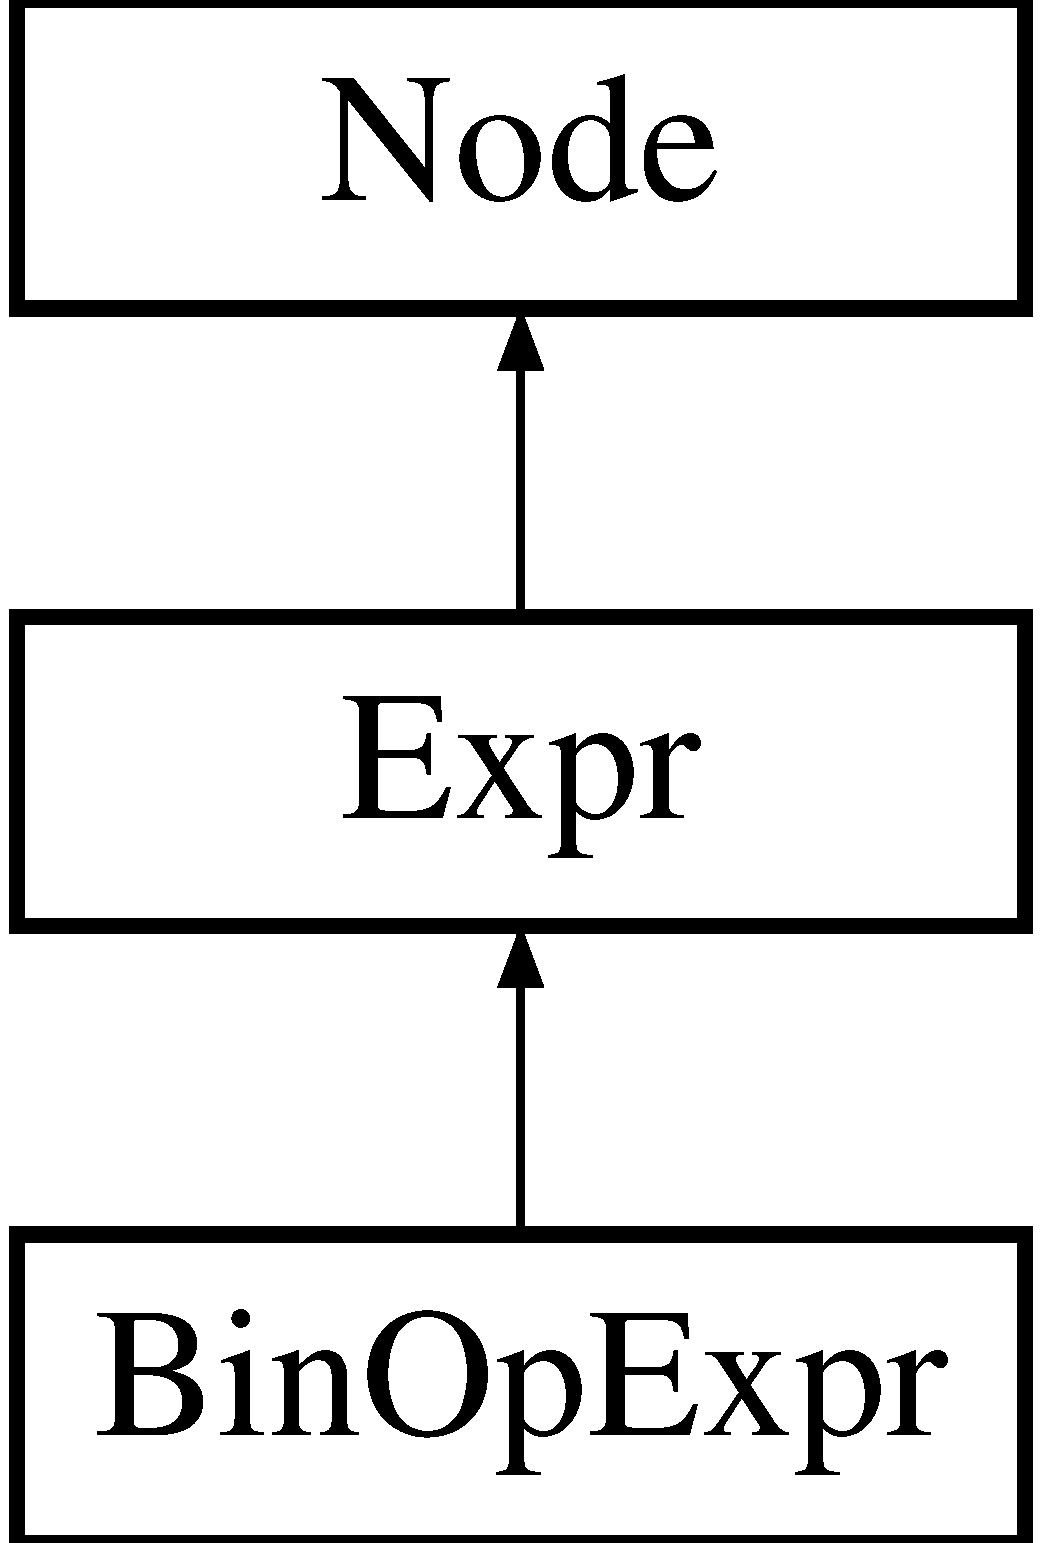
\includegraphics[height=3.000000cm]{classBinOpExpr}
\end{center}
\end{figure}
\subsection*{Public Member Functions}
\begin{DoxyCompactItemize}
\item 
\hypertarget{classBinOpExpr_a8f70bcea569210a4af6e3912c568502c}{\hyperlink{classBinOpExpr_a8f70bcea569210a4af6e3912c568502c}{Bin\-Op\-Expr} (\hyperlink{classExpr}{Expr} $\ast$\-\_\-expr1, std\-::string \-\_\-op, \hyperlink{classExpr}{Expr} $\ast$\-\_\-expr2)}\label{classBinOpExpr_a8f70bcea569210a4af6e3912c568502c}

\begin{DoxyCompactList}\small\item\em Constructor for \hyperlink{classBinOpExpr}{Bin\-Op\-Expr} node. \end{DoxyCompactList}\item 
\hypertarget{classBinOpExpr_a695fc973bc681fcceda2f81130098649}{std\-::string \hyperlink{classBinOpExpr_a695fc973bc681fcceda2f81130098649}{unparse} ()}\label{classBinOpExpr_a695fc973bc681fcceda2f81130098649}

\begin{DoxyCompactList}\small\item\em \hyperlink{classExpr}{Expr} 'op' \hyperlink{classExpr}{Expr}. \end{DoxyCompactList}\end{DoxyCompactItemize}


The documentation for this class was generated from the following files\-:\begin{DoxyCompactItemize}
\item 
A\-S\-T.\-h\item 
A\-S\-T.\-cpp\end{DoxyCompactItemize}

\hypertarget{classBooleanExpr}{\section{Boolean\-Expr Class Reference}
\label{classBooleanExpr}\index{Boolean\-Expr@{Boolean\-Expr}}
}
Inheritance diagram for Boolean\-Expr\-:\begin{figure}[H]
\begin{center}
\leavevmode
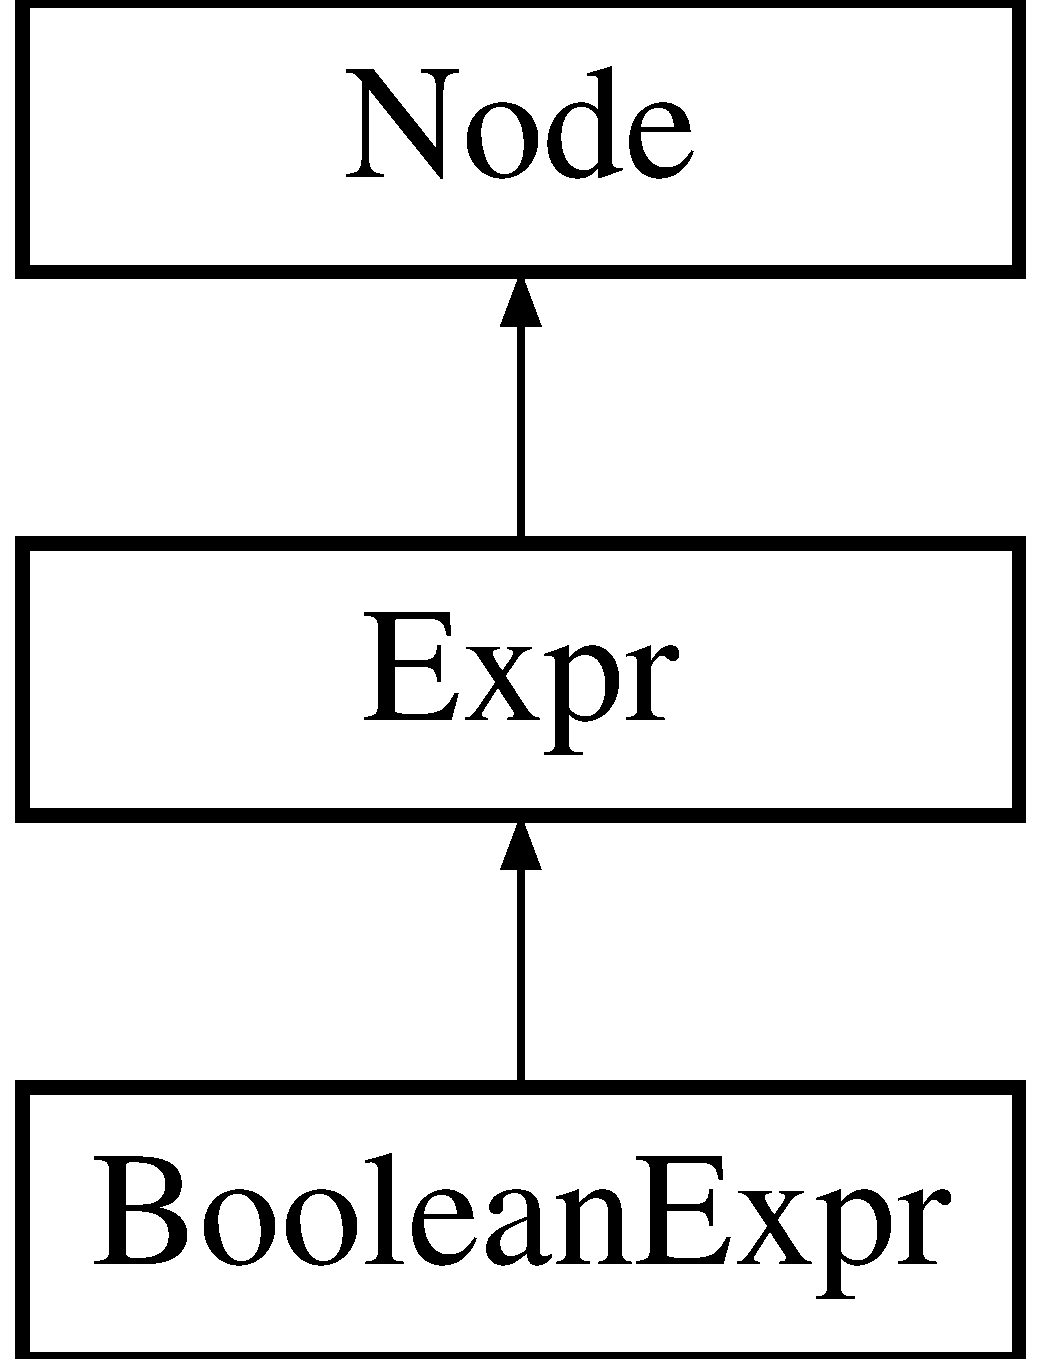
\includegraphics[height=3.000000cm]{classBooleanExpr}
\end{center}
\end{figure}
\subsection*{Public Member Functions}
\begin{DoxyCompactItemize}
\item 
\hypertarget{classBooleanExpr_a3bf7eb8048426d84900fd2047d4d5983}{\hyperlink{classBooleanExpr_a3bf7eb8048426d84900fd2047d4d5983}{Boolean\-Expr} (std\-::string \-\_\-var)}\label{classBooleanExpr_a3bf7eb8048426d84900fd2047d4d5983}

\begin{DoxyCompactList}\small\item\em Constructor for \hyperlink{classBooleanExpr}{Boolean\-Expr} node. \end{DoxyCompactList}\item 
\hypertarget{classBooleanExpr_a605d334f7d8b38d95dfd936b9fe72ca0}{std\-::string \hyperlink{classBooleanExpr_a605d334f7d8b38d95dfd936b9fe72ca0}{unparse} ()}\label{classBooleanExpr_a605d334f7d8b38d95dfd936b9fe72ca0}

\begin{DoxyCompactList}\small\item\em \hyperlink{classExpr}{Expr} 'op' \hyperlink{classExpr}{Expr}. \end{DoxyCompactList}\end{DoxyCompactItemize}


The documentation for this class was generated from the following files\-:\begin{DoxyCompactItemize}
\item 
A\-S\-T.\-h\item 
A\-S\-T.\-cpp\end{DoxyCompactItemize}

\hypertarget{classCharConstToken}{\section{Char\-Const\-Token Class Reference}
\label{classCharConstToken}\index{Char\-Const\-Token@{Char\-Const\-Token}}
}
Inheritance diagram for Char\-Const\-Token\-:\begin{figure}[H]
\begin{center}
\leavevmode
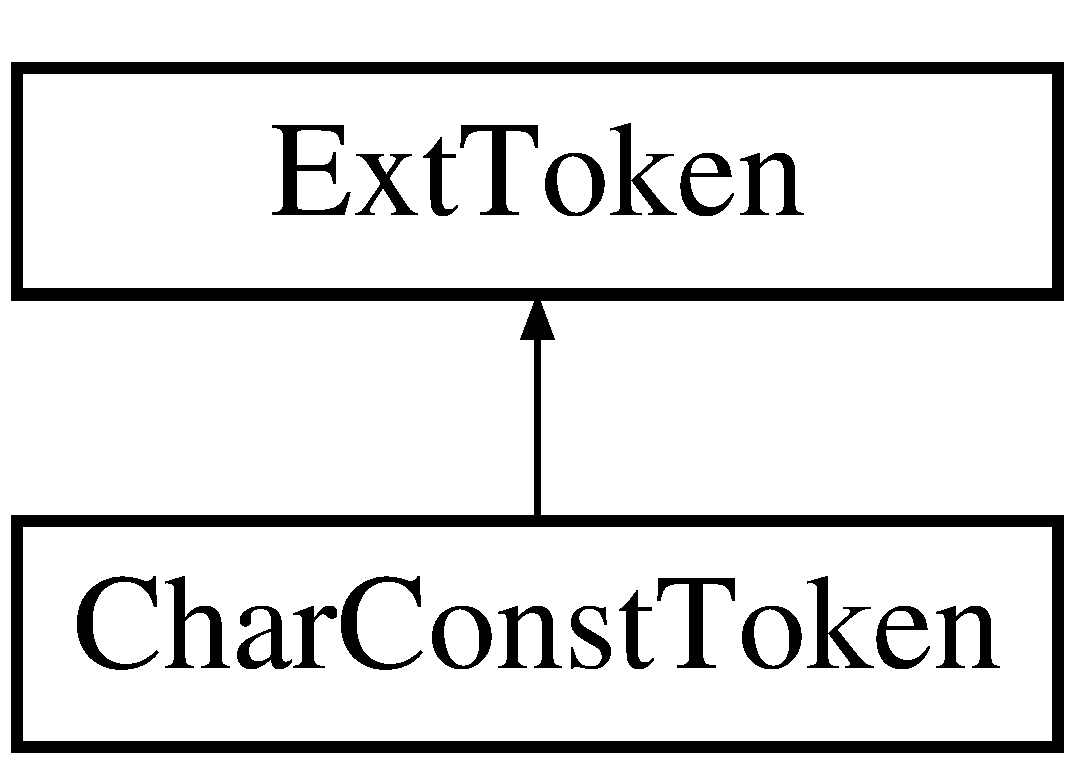
\includegraphics[height=2.000000cm]{classCharConstToken}
\end{center}
\end{figure}
\subsection*{Public Member Functions}
\begin{DoxyCompactItemize}
\item 
\hypertarget{classCharConstToken_a9dcb8d0d26c4f9c66570357641933c51}{{\bfseries Char\-Const\-Token} (\hyperlink{classParser}{Parser} $\ast$p, \hyperlink{classToken}{Token} $\ast$t)}\label{classCharConstToken_a9dcb8d0d26c4f9c66570357641933c51}

\item 
\hypertarget{classCharConstToken_a33032d6b35ef2b6ebc4db770b374ad5b}{\hyperlink{classParseResult}{Parse\-Result} {\bfseries nud} ()}\label{classCharConstToken_a33032d6b35ef2b6ebc4db770b374ad5b}

\item 
\hypertarget{classCharConstToken_addf2603d51bc2be908137f06737d8b30}{std\-::string {\bfseries description} ()}\label{classCharConstToken_addf2603d51bc2be908137f06737d8b30}

\end{DoxyCompactItemize}
\subsection*{Additional Inherited Members}


The documentation for this class was generated from the following file\-:\begin{DoxyCompactItemize}
\item 
ext\-Token.\-h\end{DoxyCompactItemize}

\hypertarget{classDashToken}{\section{Dash\-Token Class Reference}
\label{classDashToken}\index{Dash\-Token@{Dash\-Token}}
}
Inheritance diagram for Dash\-Token\-:\begin{figure}[H]
\begin{center}
\leavevmode
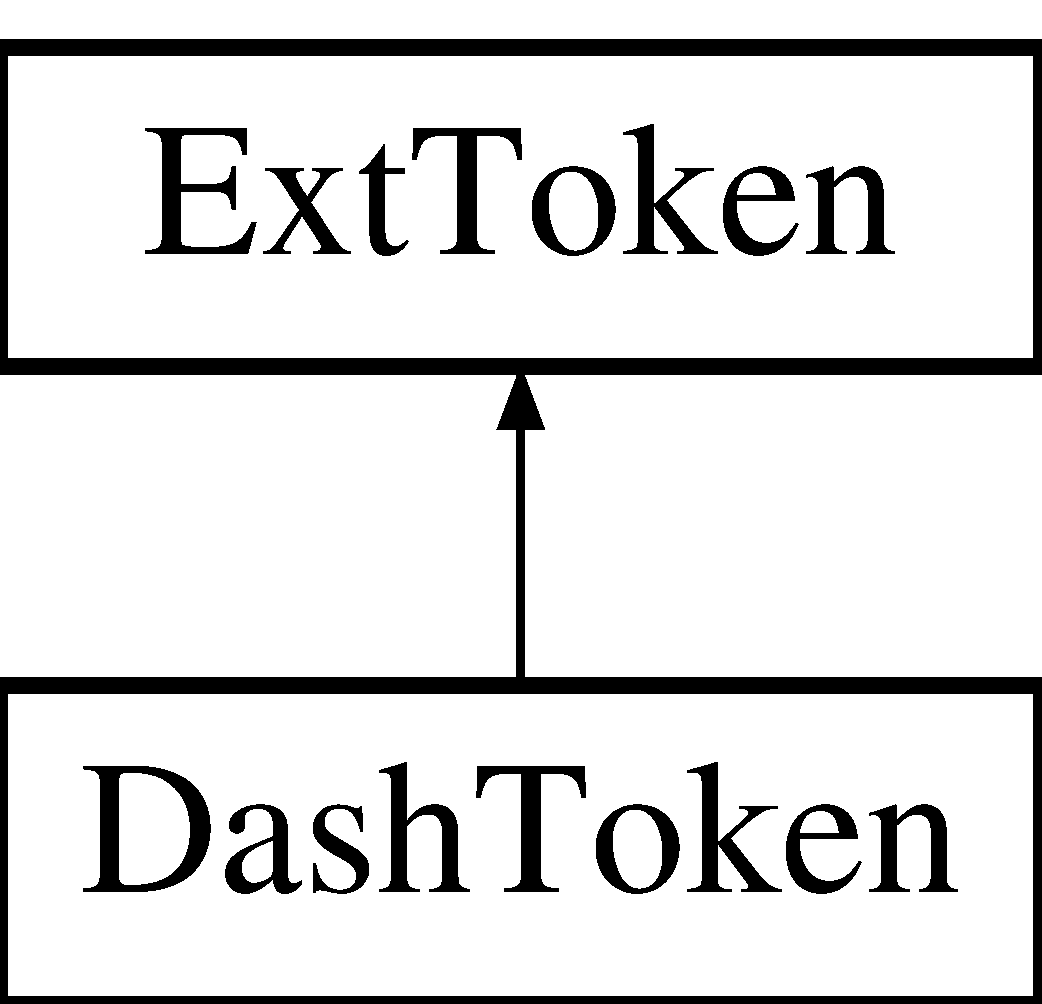
\includegraphics[height=2.000000cm]{classDashToken}
\end{center}
\end{figure}
\subsection*{Public Member Functions}
\begin{DoxyCompactItemize}
\item 
\hypertarget{classDashToken_a9570d66563405c728e679b63a44e53e2}{{\bfseries Dash\-Token} (\hyperlink{classParser}{Parser} $\ast$p, \hyperlink{classToken}{Token} $\ast$t)}\label{classDashToken_a9570d66563405c728e679b63a44e53e2}

\item 
\hypertarget{classDashToken_a703ca6afcd05ac4688c66b82e177bdbc}{\hyperlink{classParseResult}{Parse\-Result} {\bfseries led} (\hyperlink{classParseResult}{Parse\-Result} left)}\label{classDashToken_a703ca6afcd05ac4688c66b82e177bdbc}

\item 
\hypertarget{classDashToken_a02d79abb30dcab20081edb8e969885d2}{std\-::string {\bfseries description} ()}\label{classDashToken_a02d79abb30dcab20081edb8e969885d2}

\item 
\hypertarget{classDashToken_a1cf877584a85c06e884a182744e92b39}{int {\bfseries lbp} ()}\label{classDashToken_a1cf877584a85c06e884a182744e92b39}

\end{DoxyCompactItemize}
\subsection*{Additional Inherited Members}


The documentation for this class was generated from the following file\-:\begin{DoxyCompactItemize}
\item 
ext\-Token.\-h\end{DoxyCompactItemize}

\hypertarget{classDecl}{\section{Decl Class Reference}
\label{classDecl}\index{Decl@{Decl}}
}
Inheritance diagram for Decl\-:\begin{figure}[H]
\begin{center}
\leavevmode
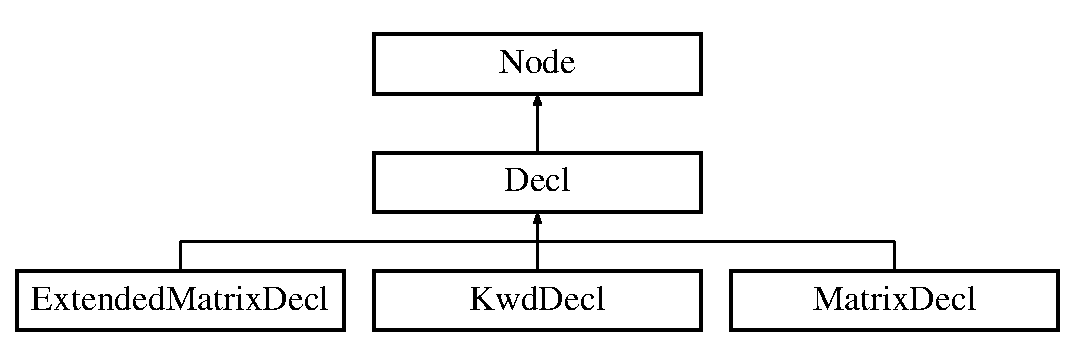
\includegraphics[height=3.000000cm]{classDecl}
\end{center}
\end{figure}
\subsection*{Additional Inherited Members}


The documentation for this class was generated from the following file\-:\begin{DoxyCompactItemize}
\item 
A\-S\-T.\-h\end{DoxyCompactItemize}

\hypertarget{classEmptyStmts}{\section{Empty\-Stmts Class Reference}
\label{classEmptyStmts}\index{Empty\-Stmts@{Empty\-Stmts}}
}
Inheritance diagram for Empty\-Stmts\-:\begin{figure}[H]
\begin{center}
\leavevmode
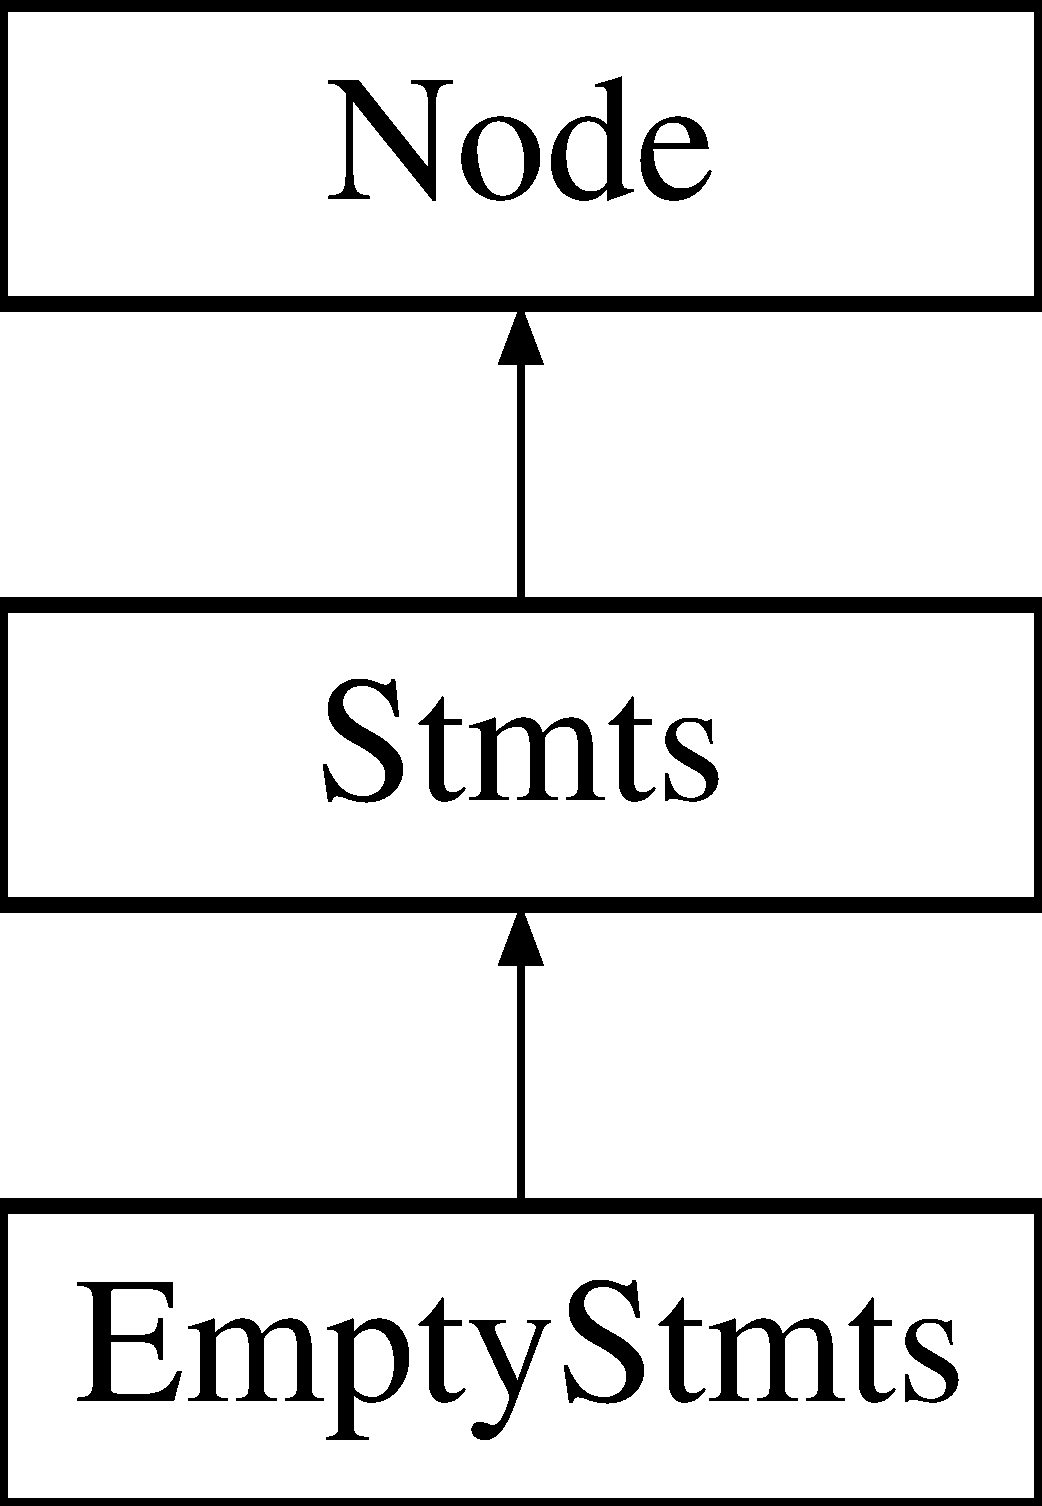
\includegraphics[height=3.000000cm]{classEmptyStmts}
\end{center}
\end{figure}
\subsection*{Public Member Functions}
\begin{DoxyCompactItemize}
\item 
\hypertarget{classEmptyStmts_aec1fdeb62d294b8fedf55ff234fcacf5}{\hyperlink{classEmptyStmts_aec1fdeb62d294b8fedf55ff234fcacf5}{Empty\-Stmts} ()}\label{classEmptyStmts_aec1fdeb62d294b8fedf55ff234fcacf5}

\begin{DoxyCompactList}\small\item\em Constructor for \hyperlink{classEmptyStmts}{Empty\-Stmts} node. \end{DoxyCompactList}\item 
\hypertarget{classEmptyStmts_a127064ef5c59227fc8452b31c65eb905}{std\-::string \hyperlink{classEmptyStmts_a127064ef5c59227fc8452b31c65eb905}{unparse} ()}\label{classEmptyStmts_a127064ef5c59227fc8452b31c65eb905}

\begin{DoxyCompactList}\small\item\em $<$$<$empty$>$$>$ \end{DoxyCompactList}\end{DoxyCompactItemize}


The documentation for this class was generated from the following files\-:\begin{DoxyCompactItemize}
\item 
A\-S\-T.\-h\item 
A\-S\-T.\-cpp\end{DoxyCompactItemize}

\hypertarget{classEndOfFileToken}{\section{End\-Of\-File\-Token Class Reference}
\label{classEndOfFileToken}\index{End\-Of\-File\-Token@{End\-Of\-File\-Token}}
}
Inheritance diagram for End\-Of\-File\-Token\-:\begin{figure}[H]
\begin{center}
\leavevmode
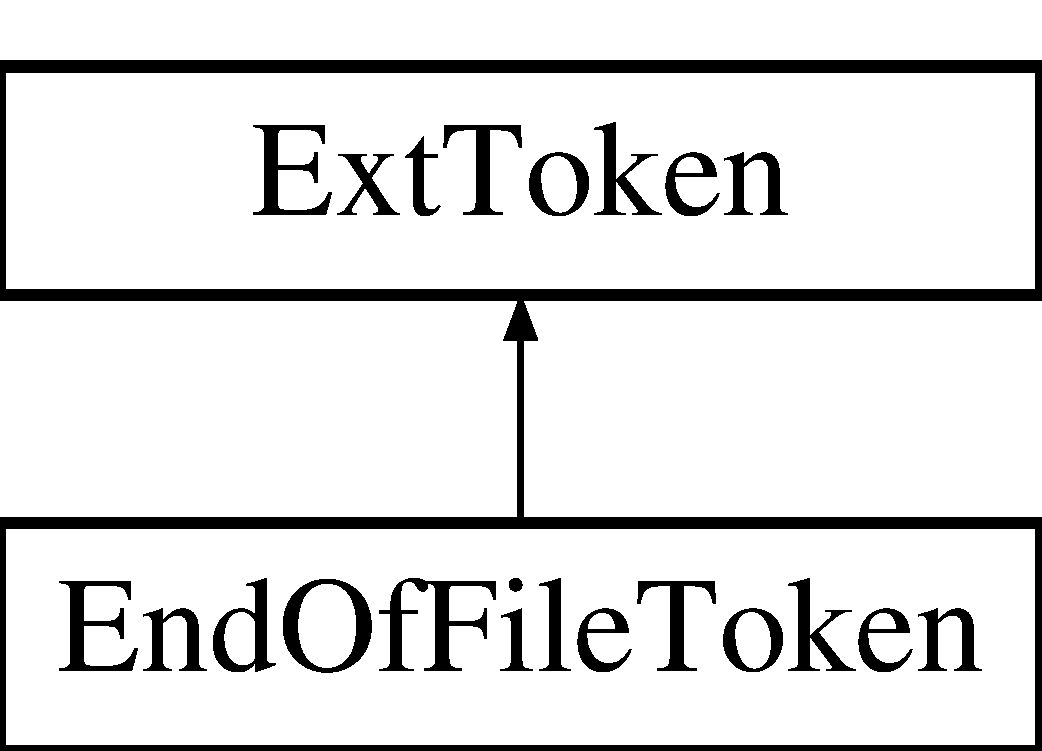
\includegraphics[height=2.000000cm]{classEndOfFileToken}
\end{center}
\end{figure}
\subsection*{Public Member Functions}
\begin{DoxyCompactItemize}
\item 
\hypertarget{classEndOfFileToken_a5c093bc13648a4f4df525ea4242e59d9}{{\bfseries End\-Of\-File\-Token} (\hyperlink{classParser}{Parser} $\ast$p, \hyperlink{classToken}{Token} $\ast$t)}\label{classEndOfFileToken_a5c093bc13648a4f4df525ea4242e59d9}

\item 
\hypertarget{classEndOfFileToken_a918312b101ca8cc7fb5ba4e56bc12b58}{std\-::string {\bfseries description} ()}\label{classEndOfFileToken_a918312b101ca8cc7fb5ba4e56bc12b58}

\end{DoxyCompactItemize}
\subsection*{Additional Inherited Members}


The documentation for this class was generated from the following file\-:\begin{DoxyCompactItemize}
\item 
ext\-Token.\-h\end{DoxyCompactItemize}

\hypertarget{classExpr}{\section{Expr Class Reference}
\label{classExpr}\index{Expr@{Expr}}
}
Inheritance diagram for Expr\-:\begin{figure}[H]
\begin{center}
\leavevmode
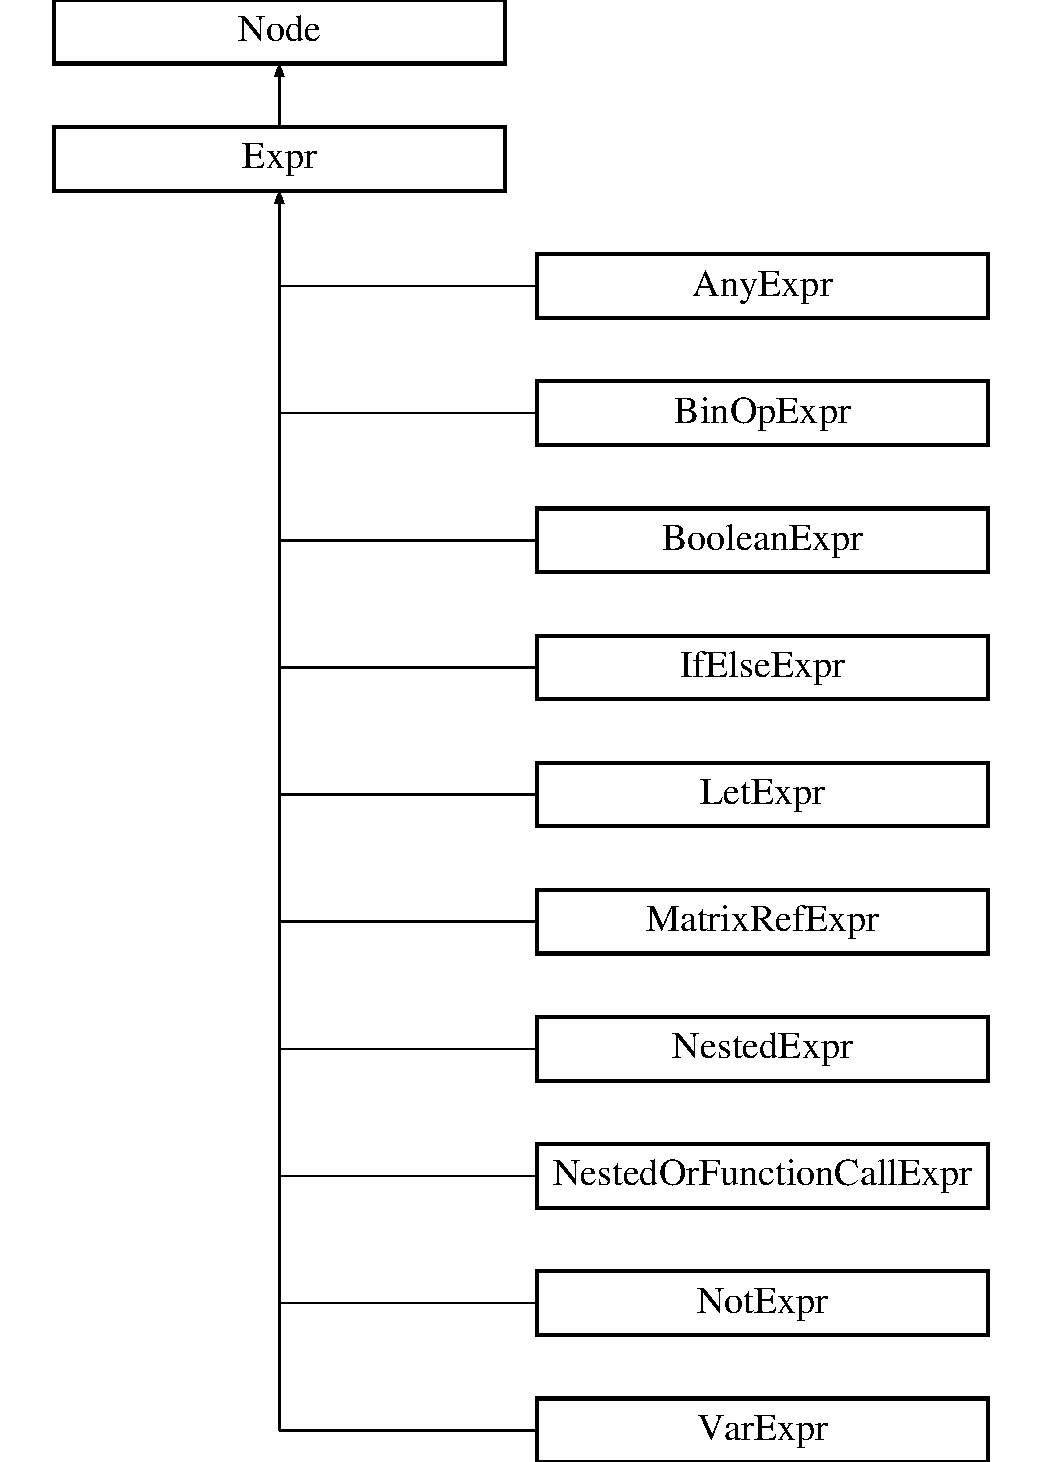
\includegraphics[height=12.000000cm]{classExpr}
\end{center}
\end{figure}
\subsection*{Additional Inherited Members}


The documentation for this class was generated from the following file\-:\begin{DoxyCompactItemize}
\item 
A\-S\-T.\-h\end{DoxyCompactItemize}

\hypertarget{classExtendedAssignStmt}{\section{Extended\-Assign\-Stmt Class Reference}
\label{classExtendedAssignStmt}\index{Extended\-Assign\-Stmt@{Extended\-Assign\-Stmt}}
}
Inheritance diagram for Extended\-Assign\-Stmt\-:\begin{figure}[H]
\begin{center}
\leavevmode
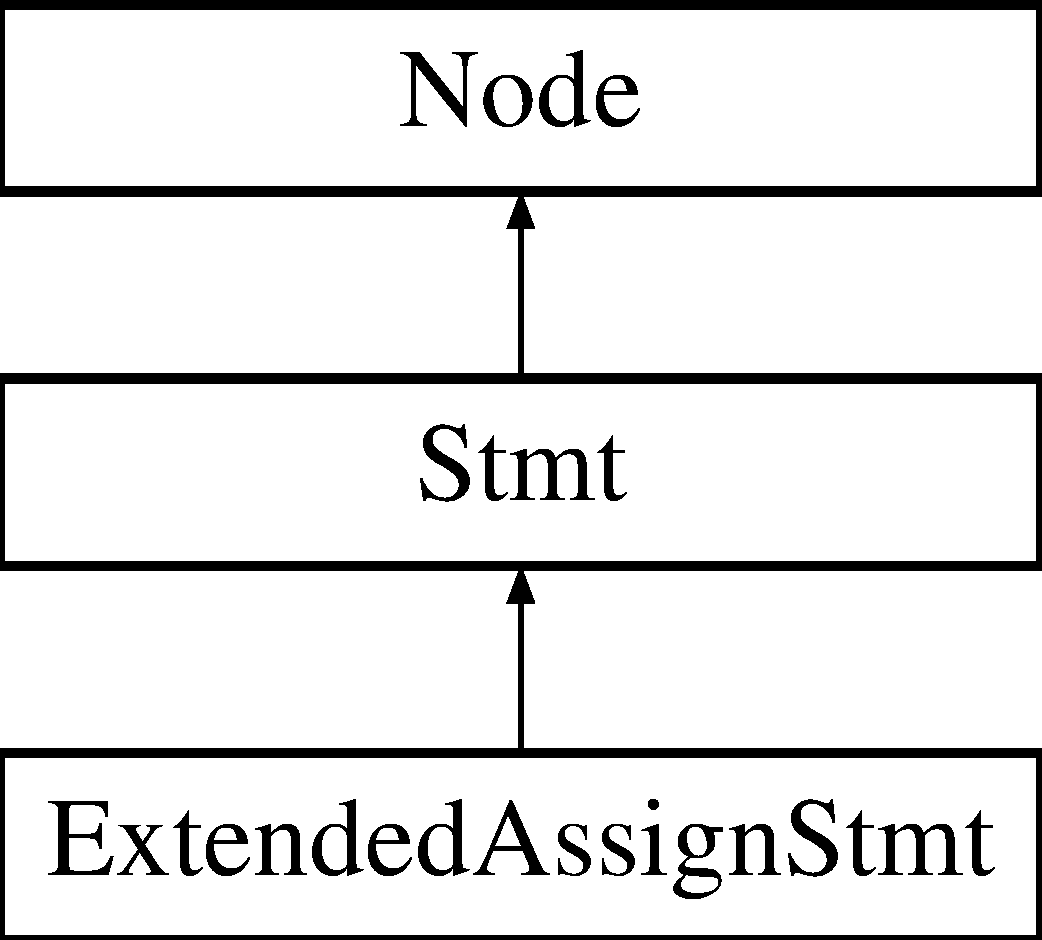
\includegraphics[height=3.000000cm]{classExtendedAssignStmt}
\end{center}
\end{figure}
\subsection*{Public Member Functions}
\begin{DoxyCompactItemize}
\item 
\hypertarget{classExtendedAssignStmt_a3623f072f66a39e54ed8c61ea72b0edf}{{\bfseries Extended\-Assign\-Stmt} (std\-::string \-\_\-varname, \hyperlink{classExpr}{Expr} $\ast$\-\_\-expr1, \hyperlink{classExpr}{Expr} $\ast$\-\_\-expr2, \hyperlink{classExpr}{Expr} $\ast$\-\_\-expr3)}\label{classExtendedAssignStmt_a3623f072f66a39e54ed8c61ea72b0edf}

\item 
\hypertarget{classExtendedAssignStmt_ab5437e004d97aa79df0a327dea7f93dc}{std\-::string \hyperlink{classExtendedAssignStmt_ab5437e004d97aa79df0a327dea7f93dc}{unparse} ()}\label{classExtendedAssignStmt_ab5437e004d97aa79df0a327dea7f93dc}

\begin{DoxyCompactList}\small\item\em var\-Name '\mbox{[}' \hyperlink{classExpr}{Expr} ',' \hyperlink{classExpr}{Expr} '\mbox{]}' '=' \hyperlink{classExpr}{Expr} ';' \end{DoxyCompactList}\end{DoxyCompactItemize}


The documentation for this class was generated from the following files\-:\begin{DoxyCompactItemize}
\item 
A\-S\-T.\-h\item 
A\-S\-T.\-cpp\end{DoxyCompactItemize}

\hypertarget{classExtendedMatrixDecl}{\section{Extended\-Matrix\-Decl Class Reference}
\label{classExtendedMatrixDecl}\index{Extended\-Matrix\-Decl@{Extended\-Matrix\-Decl}}
}
Inheritance diagram for Extended\-Matrix\-Decl\-:\begin{figure}[H]
\begin{center}
\leavevmode
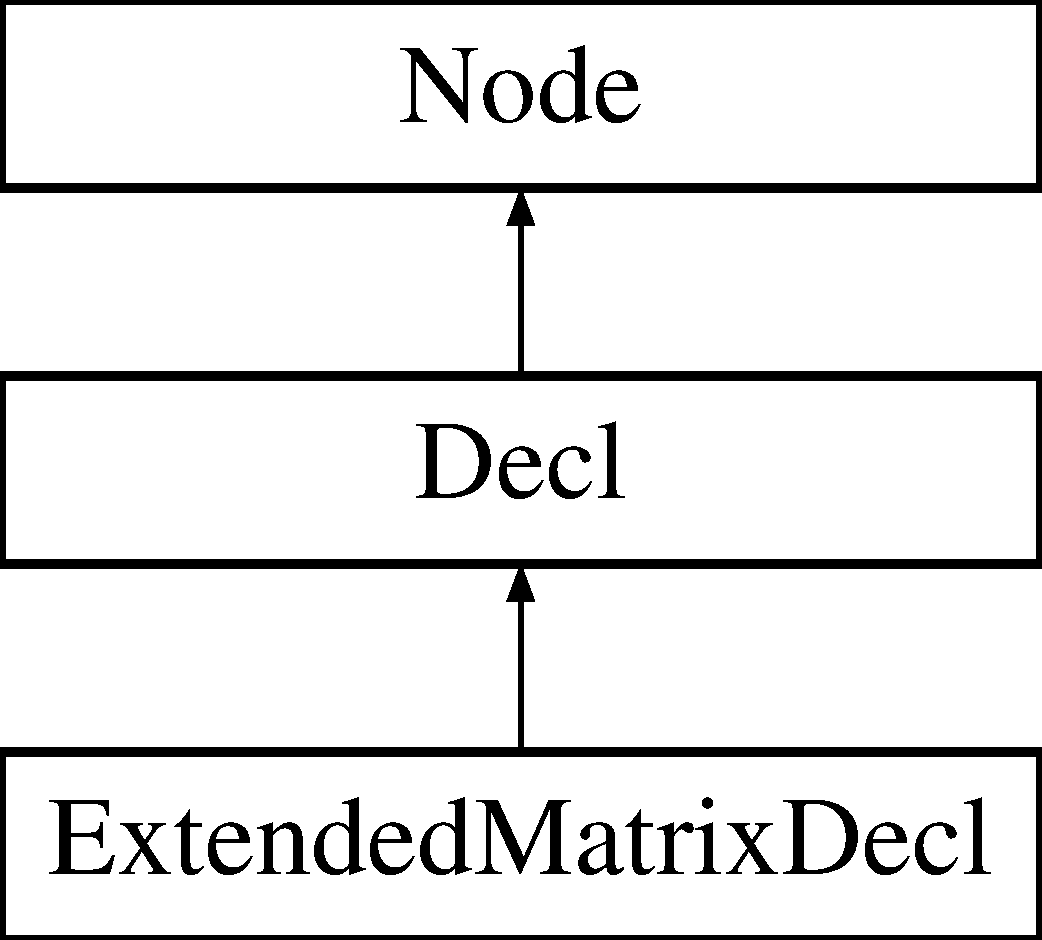
\includegraphics[height=3.000000cm]{classExtendedMatrixDecl}
\end{center}
\end{figure}
\subsection*{Public Member Functions}
\begin{DoxyCompactItemize}
\item 
\hypertarget{classExtendedMatrixDecl_a6f62ebcd1a88e224ab02ac7175c99d45}{\hyperlink{classExtendedMatrixDecl_a6f62ebcd1a88e224ab02ac7175c99d45}{Extended\-Matrix\-Decl} (std\-::string \-\_\-varname1, \hyperlink{classExpr}{Expr} $\ast$\-\_\-expr1, \hyperlink{classExpr}{Expr} $\ast$\-\_\-expr2, std\-::string \-\_\-varname2, std\-::string \-\_\-varname3, \hyperlink{classExpr}{Expr} $\ast$\-\_\-expr3)}\label{classExtendedMatrixDecl_a6f62ebcd1a88e224ab02ac7175c99d45}

\begin{DoxyCompactList}\small\item\em Constructor for \hyperlink{classExtendedMatrixDecl}{Extended\-Matrix\-Decl} node. \end{DoxyCompactList}\item 
\hypertarget{classExtendedMatrixDecl_ae748f367ce4f92b68a11f504e98bf97f}{std\-::string \hyperlink{classExtendedMatrixDecl_ae748f367ce4f92b68a11f504e98bf97f}{unparse} ()}\label{classExtendedMatrixDecl_ae748f367ce4f92b68a11f504e98bf97f}

\begin{DoxyCompactList}\small\item\em 'Matrix' var\-Name '\mbox{[}' \hyperlink{classExpr}{Expr} ',' \hyperlink{classExpr}{Expr} '\mbox{]}' var\-Name ',' var\-Name '=' \hyperlink{classExpr}{Expr} ';' \end{DoxyCompactList}\end{DoxyCompactItemize}


The documentation for this class was generated from the following files\-:\begin{DoxyCompactItemize}
\item 
A\-S\-T.\-h\item 
A\-S\-T.\-cpp\end{DoxyCompactItemize}

\hypertarget{classExtToken}{\section{Ext\-Token Class Reference}
\label{classExtToken}\index{Ext\-Token@{Ext\-Token}}
}
Inheritance diagram for Ext\-Token\-:\begin{figure}[H]
\begin{center}
\leavevmode
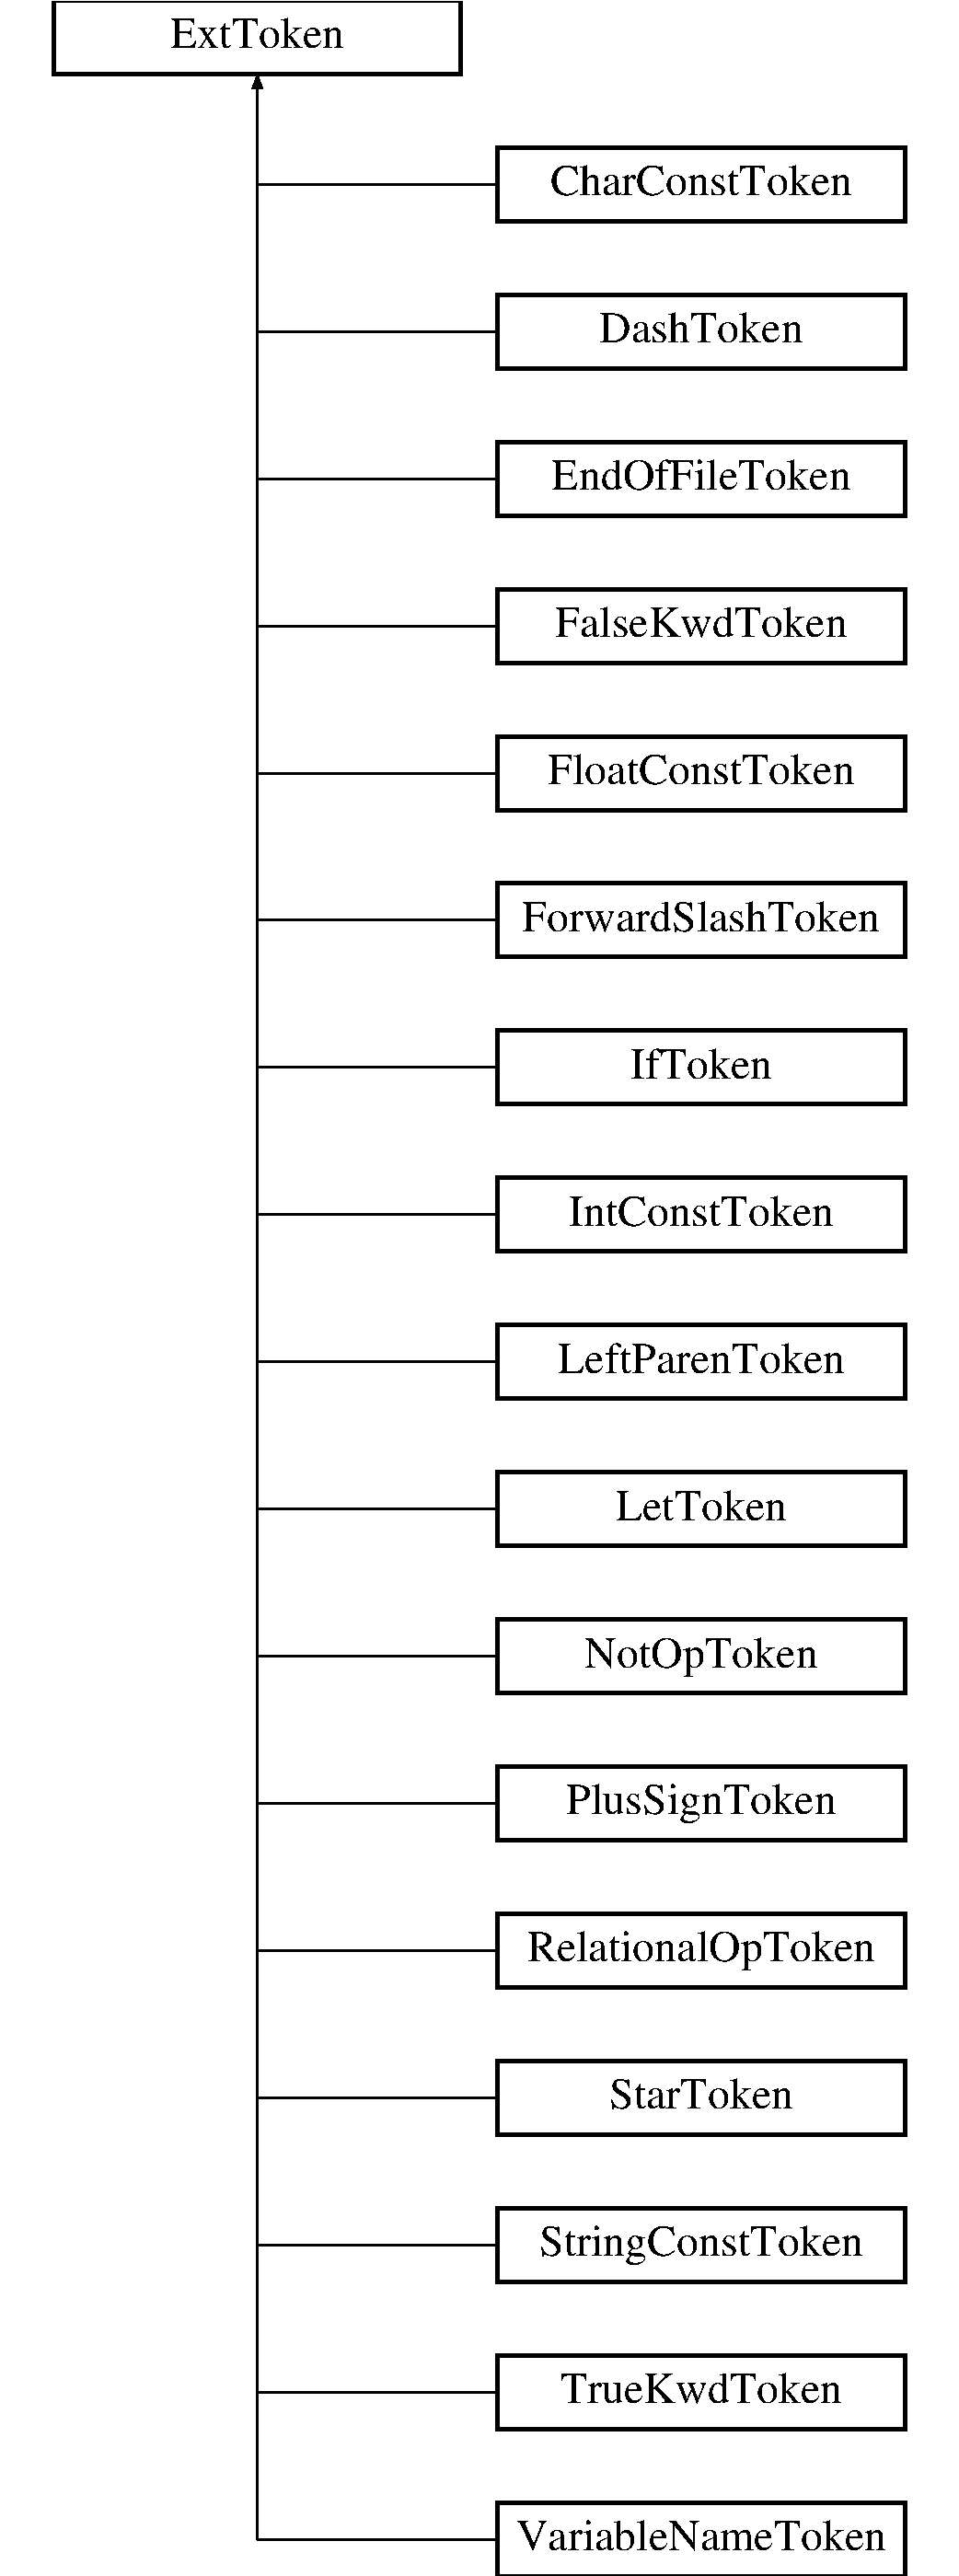
\includegraphics[height=12.000000cm]{classExtToken}
\end{center}
\end{figure}
\subsection*{Public Member Functions}
\begin{DoxyCompactItemize}
\item 
\hypertarget{classExtToken_a45a27528f391faf5679b7b30563ce846}{{\bfseries Ext\-Token} (\hyperlink{classParser}{Parser} $\ast$p, \hyperlink{classToken}{Token} $\ast$t)}\label{classExtToken_a45a27528f391faf5679b7b30563ce846}

\item 
\hypertarget{classExtToken_afa8972152abec42cd52b6f6f70a9a179}{{\bfseries Ext\-Token} (\hyperlink{classParser}{Parser} $\ast$p, \hyperlink{classToken}{Token} $\ast$t, std\-::string d)}\label{classExtToken_afa8972152abec42cd52b6f6f70a9a179}

\item 
\hypertarget{classExtToken_a5c21a5ffe91f212085259126652ab77c}{virtual \hyperlink{classParseResult}{Parse\-Result} {\bfseries nud} ()}\label{classExtToken_a5c21a5ffe91f212085259126652ab77c}

\item 
\hypertarget{classExtToken_afb2c9b0040e198d1d8aa2e041c5a7211}{virtual \hyperlink{classParseResult}{Parse\-Result} {\bfseries led} (\hyperlink{classParseResult}{Parse\-Result} left)}\label{classExtToken_afb2c9b0040e198d1d8aa2e041c5a7211}

\item 
\hypertarget{classExtToken_a6c0d61faa058b71147dd54bacee1db94}{virtual int {\bfseries lbp} ()}\label{classExtToken_a6c0d61faa058b71147dd54bacee1db94}

\item 
\hypertarget{classExtToken_a4ab6e72ac23235650b1756f794172ebb}{virtual std\-::string {\bfseries description} ()}\label{classExtToken_a4ab6e72ac23235650b1756f794172ebb}

\end{DoxyCompactItemize}
\subsection*{Public Attributes}
\begin{DoxyCompactItemize}
\item 
\hypertarget{classExtToken_a5af1643a542ef7ee8ca0f82706383ae3}{std\-::string {\bfseries lexeme}}\label{classExtToken_a5af1643a542ef7ee8ca0f82706383ae3}

\item 
\hypertarget{classExtToken_abbdaef42b65403cdc0247839ef95c875}{token\-Type {\bfseries terminal}}\label{classExtToken_abbdaef42b65403cdc0247839ef95c875}

\item 
\hypertarget{classExtToken_aa02995a897183b2a6ef758e541534e46}{\hyperlink{classExtToken}{Ext\-Token} $\ast$ {\bfseries next}}\label{classExtToken_aa02995a897183b2a6ef758e541534e46}

\item 
\hypertarget{classExtToken_af70d22156d5f8e855a8b0d92a82706ba}{\hyperlink{classParser}{Parser} $\ast$ {\bfseries parser}}\label{classExtToken_af70d22156d5f8e855a8b0d92a82706ba}

\end{DoxyCompactItemize}


The documentation for this class was generated from the following file\-:\begin{DoxyCompactItemize}
\item 
ext\-Token.\-h\end{DoxyCompactItemize}

\hypertarget{classFalseKwdToken}{\section{False\-Kwd\-Token Class Reference}
\label{classFalseKwdToken}\index{False\-Kwd\-Token@{False\-Kwd\-Token}}
}
Inheritance diagram for False\-Kwd\-Token\-:\begin{figure}[H]
\begin{center}
\leavevmode
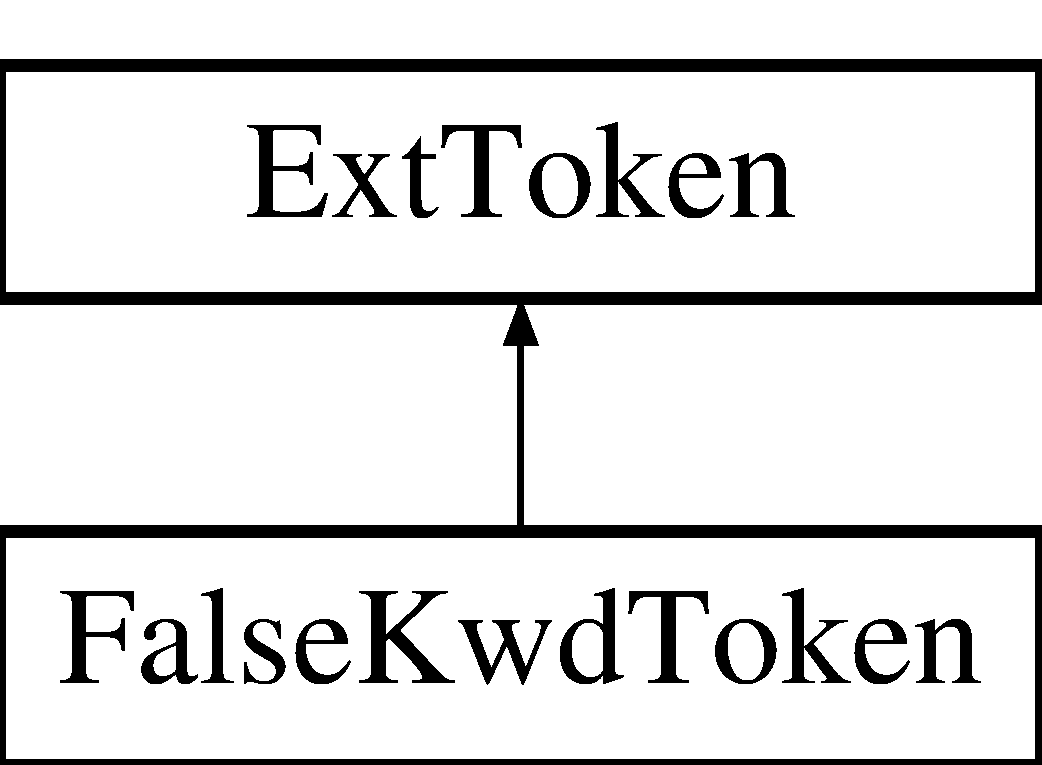
\includegraphics[height=2.000000cm]{classFalseKwdToken}
\end{center}
\end{figure}
\subsection*{Public Member Functions}
\begin{DoxyCompactItemize}
\item 
\hypertarget{classFalseKwdToken_add6402d29fd7b22253a0dc73370597e4}{{\bfseries False\-Kwd\-Token} (\hyperlink{classParser}{Parser} $\ast$p, \hyperlink{classToken}{Token} $\ast$t)}\label{classFalseKwdToken_add6402d29fd7b22253a0dc73370597e4}

\item 
\hypertarget{classFalseKwdToken_adc06b0433535d552c1e7f8076d756fb3}{\hyperlink{classParseResult}{Parse\-Result} {\bfseries nud} ()}\label{classFalseKwdToken_adc06b0433535d552c1e7f8076d756fb3}

\item 
\hypertarget{classFalseKwdToken_a8351fad7090214687138e113b5a581f1}{std\-::string {\bfseries description} ()}\label{classFalseKwdToken_a8351fad7090214687138e113b5a581f1}

\end{DoxyCompactItemize}
\subsection*{Additional Inherited Members}


The documentation for this class was generated from the following file\-:\begin{DoxyCompactItemize}
\item 
ext\-Token.\-h\end{DoxyCompactItemize}

\hypertarget{classFloatConstToken}{\section{Float\-Const\-Token Class Reference}
\label{classFloatConstToken}\index{Float\-Const\-Token@{Float\-Const\-Token}}
}
Inheritance diagram for Float\-Const\-Token\-:\begin{figure}[H]
\begin{center}
\leavevmode
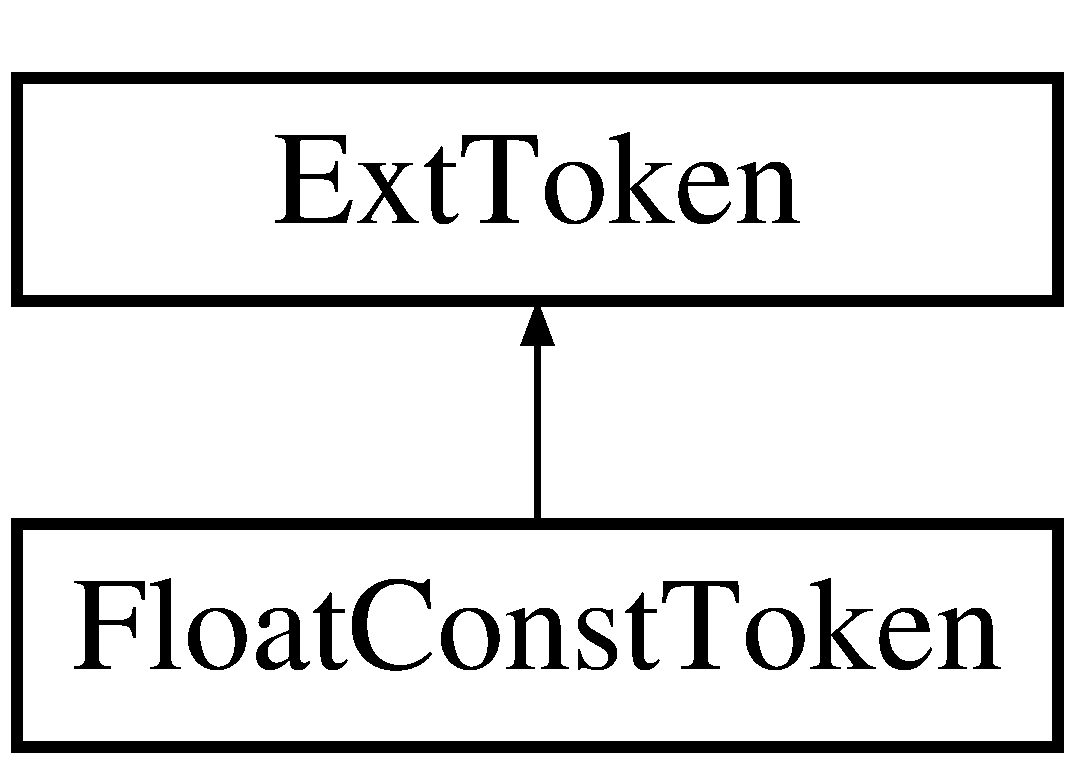
\includegraphics[height=2.000000cm]{classFloatConstToken}
\end{center}
\end{figure}
\subsection*{Public Member Functions}
\begin{DoxyCompactItemize}
\item 
\hypertarget{classFloatConstToken_aecee1d0e4e8a9410701c68c30858a4db}{{\bfseries Float\-Const\-Token} (\hyperlink{classParser}{Parser} $\ast$p, \hyperlink{classToken}{Token} $\ast$t)}\label{classFloatConstToken_aecee1d0e4e8a9410701c68c30858a4db}

\item 
\hypertarget{classFloatConstToken_a991e92ae34d0b01a3b1dd08ed01b8e6e}{\hyperlink{classParseResult}{Parse\-Result} {\bfseries nud} ()}\label{classFloatConstToken_a991e92ae34d0b01a3b1dd08ed01b8e6e}

\item 
\hypertarget{classFloatConstToken_a529b6d3ad479b0f6b940a82ba48b98c0}{std\-::string {\bfseries description} ()}\label{classFloatConstToken_a529b6d3ad479b0f6b940a82ba48b98c0}

\end{DoxyCompactItemize}
\subsection*{Additional Inherited Members}


The documentation for this class was generated from the following file\-:\begin{DoxyCompactItemize}
\item 
ext\-Token.\-h\end{DoxyCompactItemize}

\hypertarget{classForwardSlashToken}{\section{Forward\-Slash\-Token Class Reference}
\label{classForwardSlashToken}\index{Forward\-Slash\-Token@{Forward\-Slash\-Token}}
}
Inheritance diagram for Forward\-Slash\-Token\-:\begin{figure}[H]
\begin{center}
\leavevmode
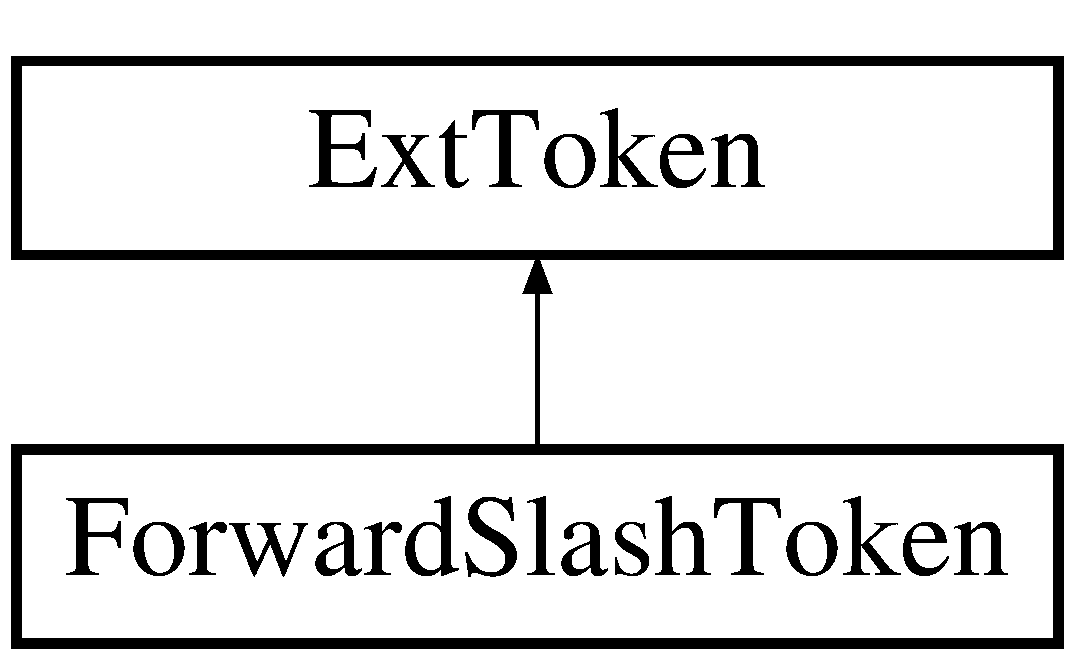
\includegraphics[height=2.000000cm]{classForwardSlashToken}
\end{center}
\end{figure}
\subsection*{Public Member Functions}
\begin{DoxyCompactItemize}
\item 
\hypertarget{classForwardSlashToken_ae818840269cd15f6f6b00929fb4eb979}{{\bfseries Forward\-Slash\-Token} (\hyperlink{classParser}{Parser} $\ast$p, \hyperlink{classToken}{Token} $\ast$t)}\label{classForwardSlashToken_ae818840269cd15f6f6b00929fb4eb979}

\item 
\hypertarget{classForwardSlashToken_ac2dda7b791ab555e4323f17baaf323e1}{\hyperlink{classParseResult}{Parse\-Result} {\bfseries led} (\hyperlink{classParseResult}{Parse\-Result} left)}\label{classForwardSlashToken_ac2dda7b791ab555e4323f17baaf323e1}

\item 
\hypertarget{classForwardSlashToken_ac27b1ab175ec08c468bd0d4c41636a5c}{std\-::string {\bfseries description} ()}\label{classForwardSlashToken_ac27b1ab175ec08c468bd0d4c41636a5c}

\item 
\hypertarget{classForwardSlashToken_ad65829044355922a291dfbfd3052b183}{int {\bfseries lbp} ()}\label{classForwardSlashToken_ad65829044355922a291dfbfd3052b183}

\end{DoxyCompactItemize}
\subsection*{Additional Inherited Members}


The documentation for this class was generated from the following file\-:\begin{DoxyCompactItemize}
\item 
ext\-Token.\-h\end{DoxyCompactItemize}

\hypertarget{classIfElseExpr}{\section{If\-Else\-Expr Class Reference}
\label{classIfElseExpr}\index{If\-Else\-Expr@{If\-Else\-Expr}}
}
Inheritance diagram for If\-Else\-Expr\-:\begin{figure}[H]
\begin{center}
\leavevmode
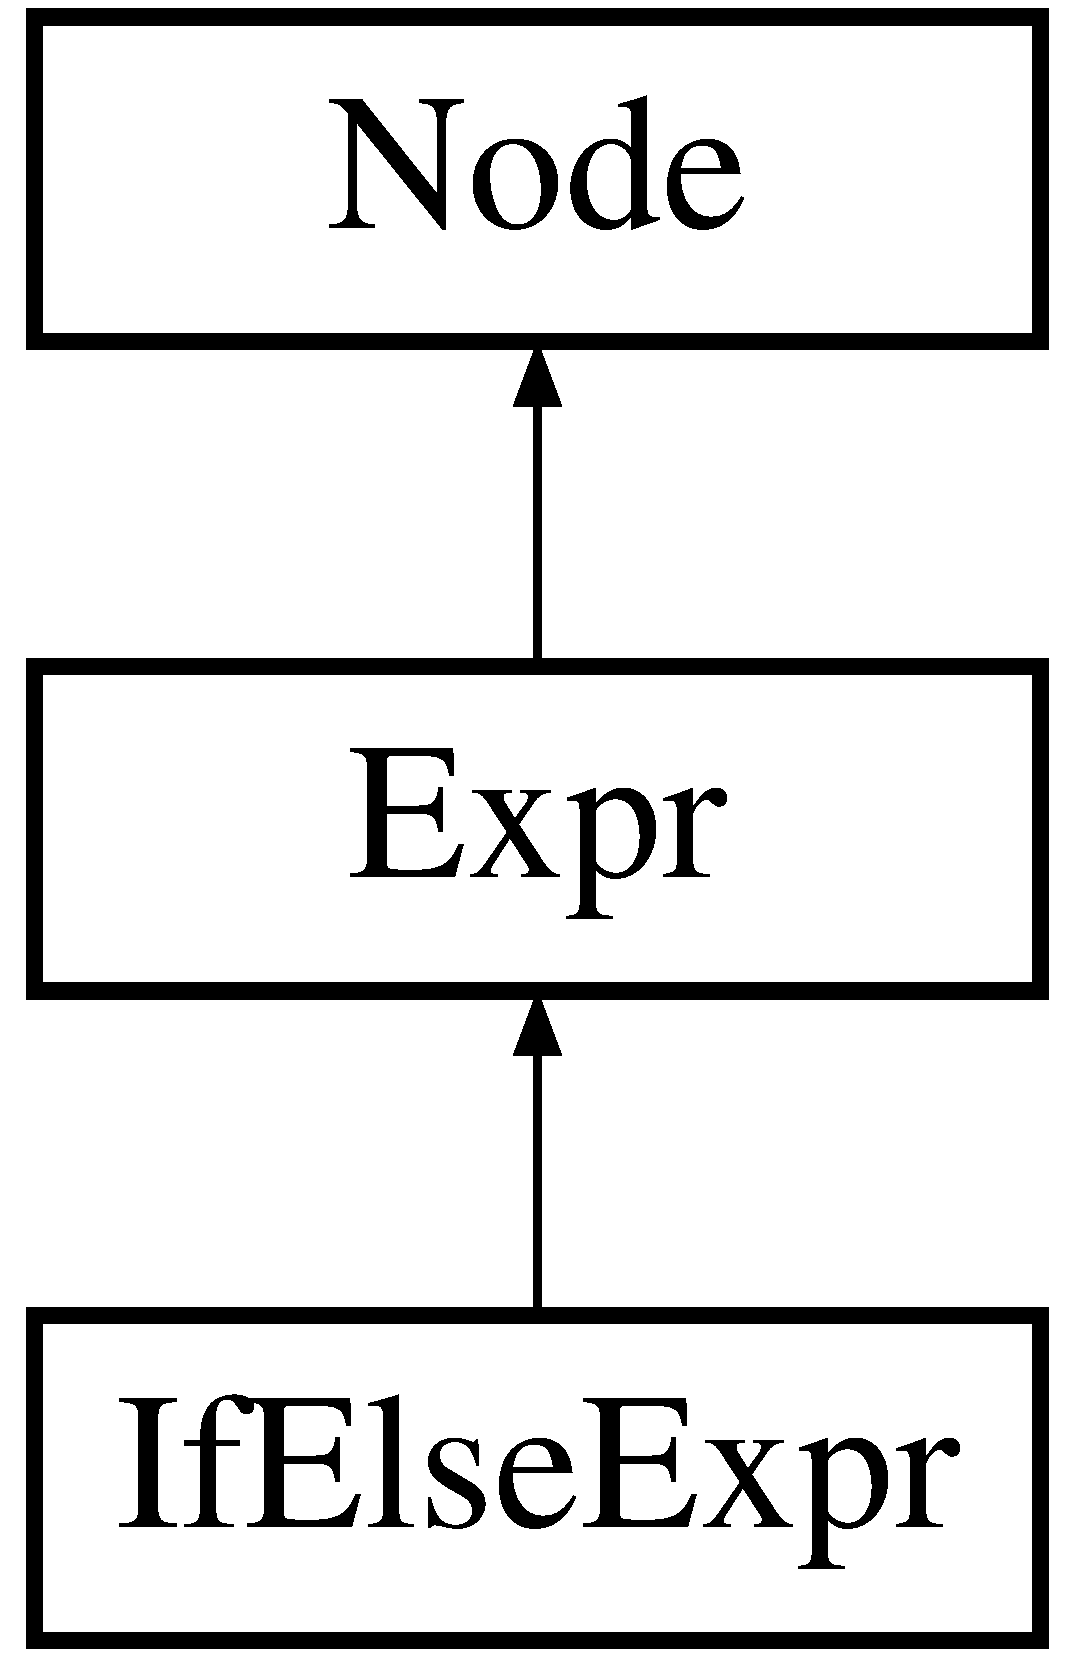
\includegraphics[height=3.000000cm]{classIfElseExpr}
\end{center}
\end{figure}
\subsection*{Public Member Functions}
\begin{DoxyCompactItemize}
\item 
\hypertarget{classIfElseExpr_a3f58094bc399d9005e1e18a2bf9447cb}{\hyperlink{classIfElseExpr_a3f58094bc399d9005e1e18a2bf9447cb}{If\-Else\-Expr} (\hyperlink{classExpr}{Expr} $\ast$\-\_\-expr1, \hyperlink{classExpr}{Expr} $\ast$\-\_\-expr2, \hyperlink{classExpr}{Expr} $\ast$\-\_\-expr3)}\label{classIfElseExpr_a3f58094bc399d9005e1e18a2bf9447cb}

\begin{DoxyCompactList}\small\item\em Constructor for \hyperlink{classIfElseExpr}{If\-Else\-Expr} node. \end{DoxyCompactList}\item 
\hypertarget{classIfElseExpr_a27fe67b8603744cdeba824b706f898fa}{std\-::string \hyperlink{classIfElseExpr_a27fe67b8603744cdeba824b706f898fa}{unparse} ()}\label{classIfElseExpr_a27fe67b8603744cdeba824b706f898fa}

\begin{DoxyCompactList}\small\item\em 'if' \hyperlink{classExpr}{Expr} 'then' \hyperlink{classExpr}{Expr} 'else' \hyperlink{classExpr}{Expr} \end{DoxyCompactList}\end{DoxyCompactItemize}


The documentation for this class was generated from the following files\-:\begin{DoxyCompactItemize}
\item 
A\-S\-T.\-h\item 
A\-S\-T.\-cpp\end{DoxyCompactItemize}

\hypertarget{classIfElseStmt}{\section{If\-Else\-Stmt Class Reference}
\label{classIfElseStmt}\index{If\-Else\-Stmt@{If\-Else\-Stmt}}
}
Inheritance diagram for If\-Else\-Stmt\-:\begin{figure}[H]
\begin{center}
\leavevmode
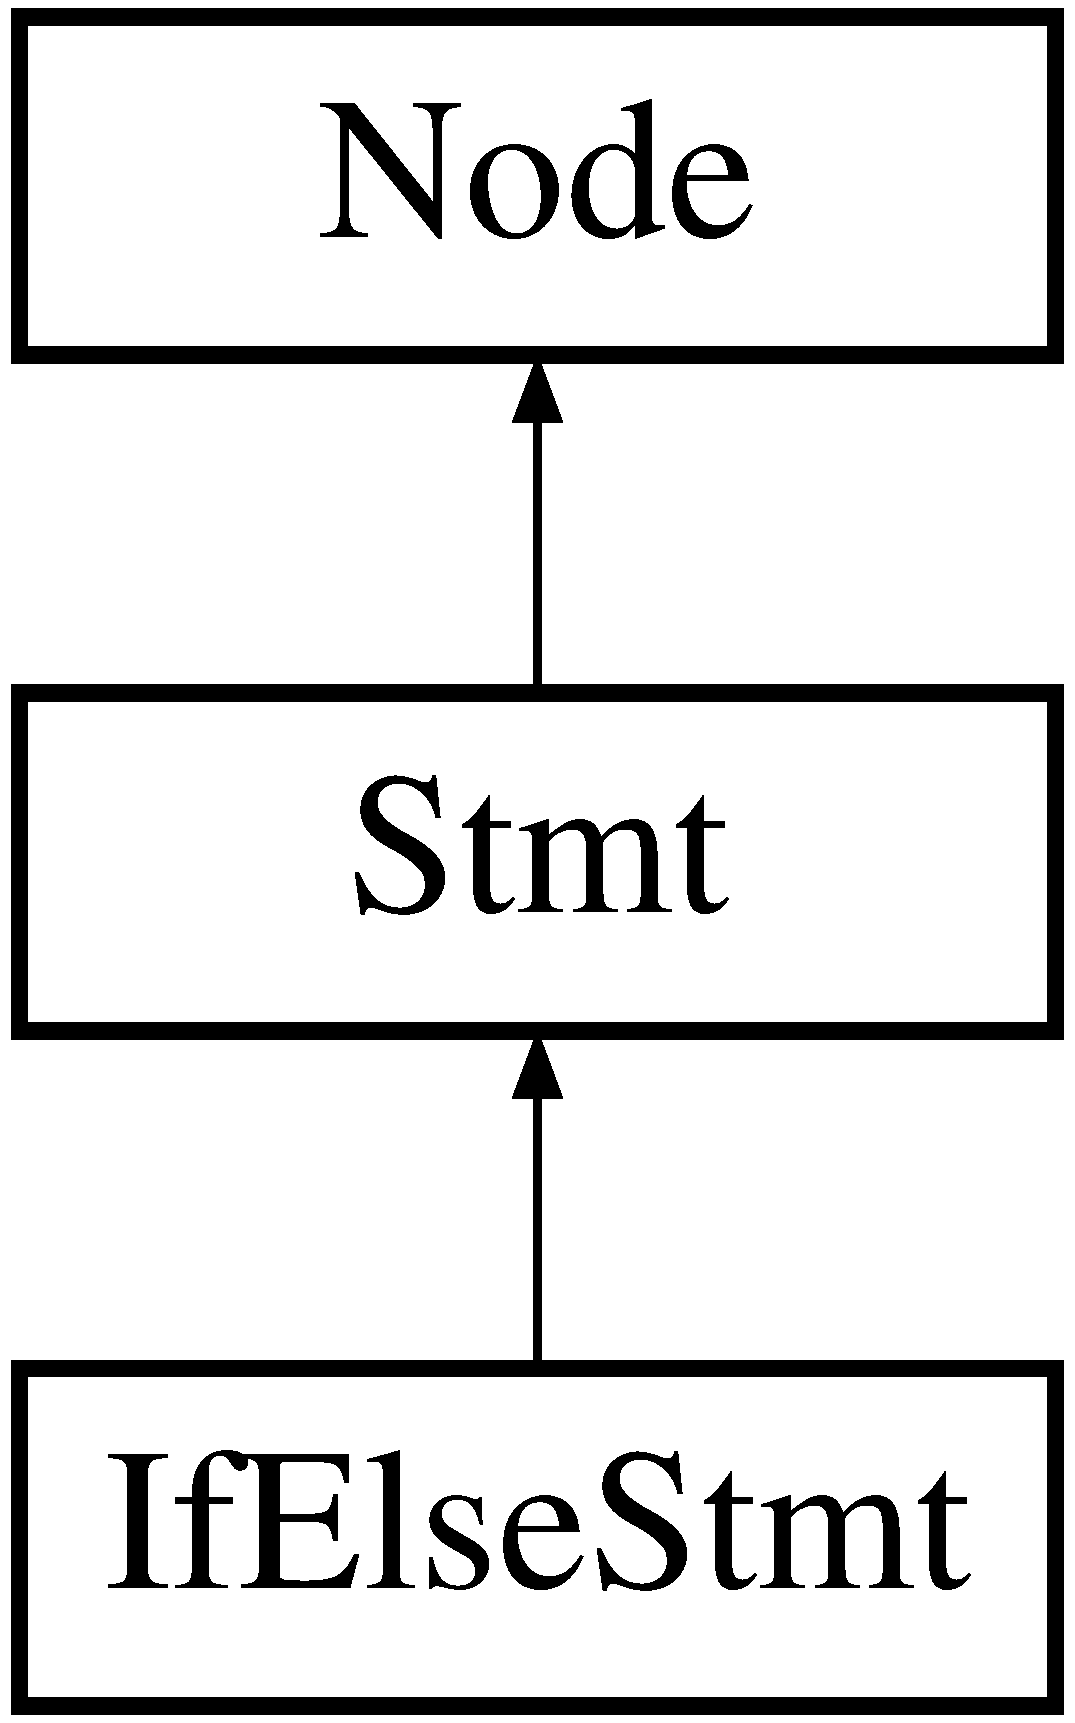
\includegraphics[height=3.000000cm]{classIfElseStmt}
\end{center}
\end{figure}
\subsection*{Public Member Functions}
\begin{DoxyCompactItemize}
\item 
\hypertarget{classIfElseStmt_a5f6717ee4f6c28af2f6d4b2efc7f5386}{\hyperlink{classIfElseStmt_a5f6717ee4f6c28af2f6d4b2efc7f5386}{If\-Else\-Stmt} (\hyperlink{classExpr}{Expr} $\ast$\-\_\-expr, \hyperlink{classStmt}{Stmt} $\ast$\-\_\-stmt, \hyperlink{classStmt}{Stmt} $\ast$\-\_\-stmt2)}\label{classIfElseStmt_a5f6717ee4f6c28af2f6d4b2efc7f5386}

\begin{DoxyCompactList}\small\item\em Constructor for \hyperlink{classIfElseStmt}{If\-Else\-Stmt} node. \end{DoxyCompactList}\item 
\hypertarget{classIfElseStmt_a82267559f8fdd5f10cf14e616f3867f2}{std\-::string \hyperlink{classIfElseStmt_a82267559f8fdd5f10cf14e616f3867f2}{unparse} ()}\label{classIfElseStmt_a82267559f8fdd5f10cf14e616f3867f2}

\begin{DoxyCompactList}\small\item\em 'if' '(' \hyperlink{classExpr}{Expr} ')' \hyperlink{classStmt}{Stmt} 'else' \hyperlink{classStmt}{Stmt} \end{DoxyCompactList}\end{DoxyCompactItemize}


The documentation for this class was generated from the following files\-:\begin{DoxyCompactItemize}
\item 
A\-S\-T.\-h\item 
A\-S\-T.\-cpp\end{DoxyCompactItemize}

\hypertarget{classIfStmt}{\section{If\-Stmt Class Reference}
\label{classIfStmt}\index{If\-Stmt@{If\-Stmt}}
}
Inheritance diagram for If\-Stmt\-:\begin{figure}[H]
\begin{center}
\leavevmode
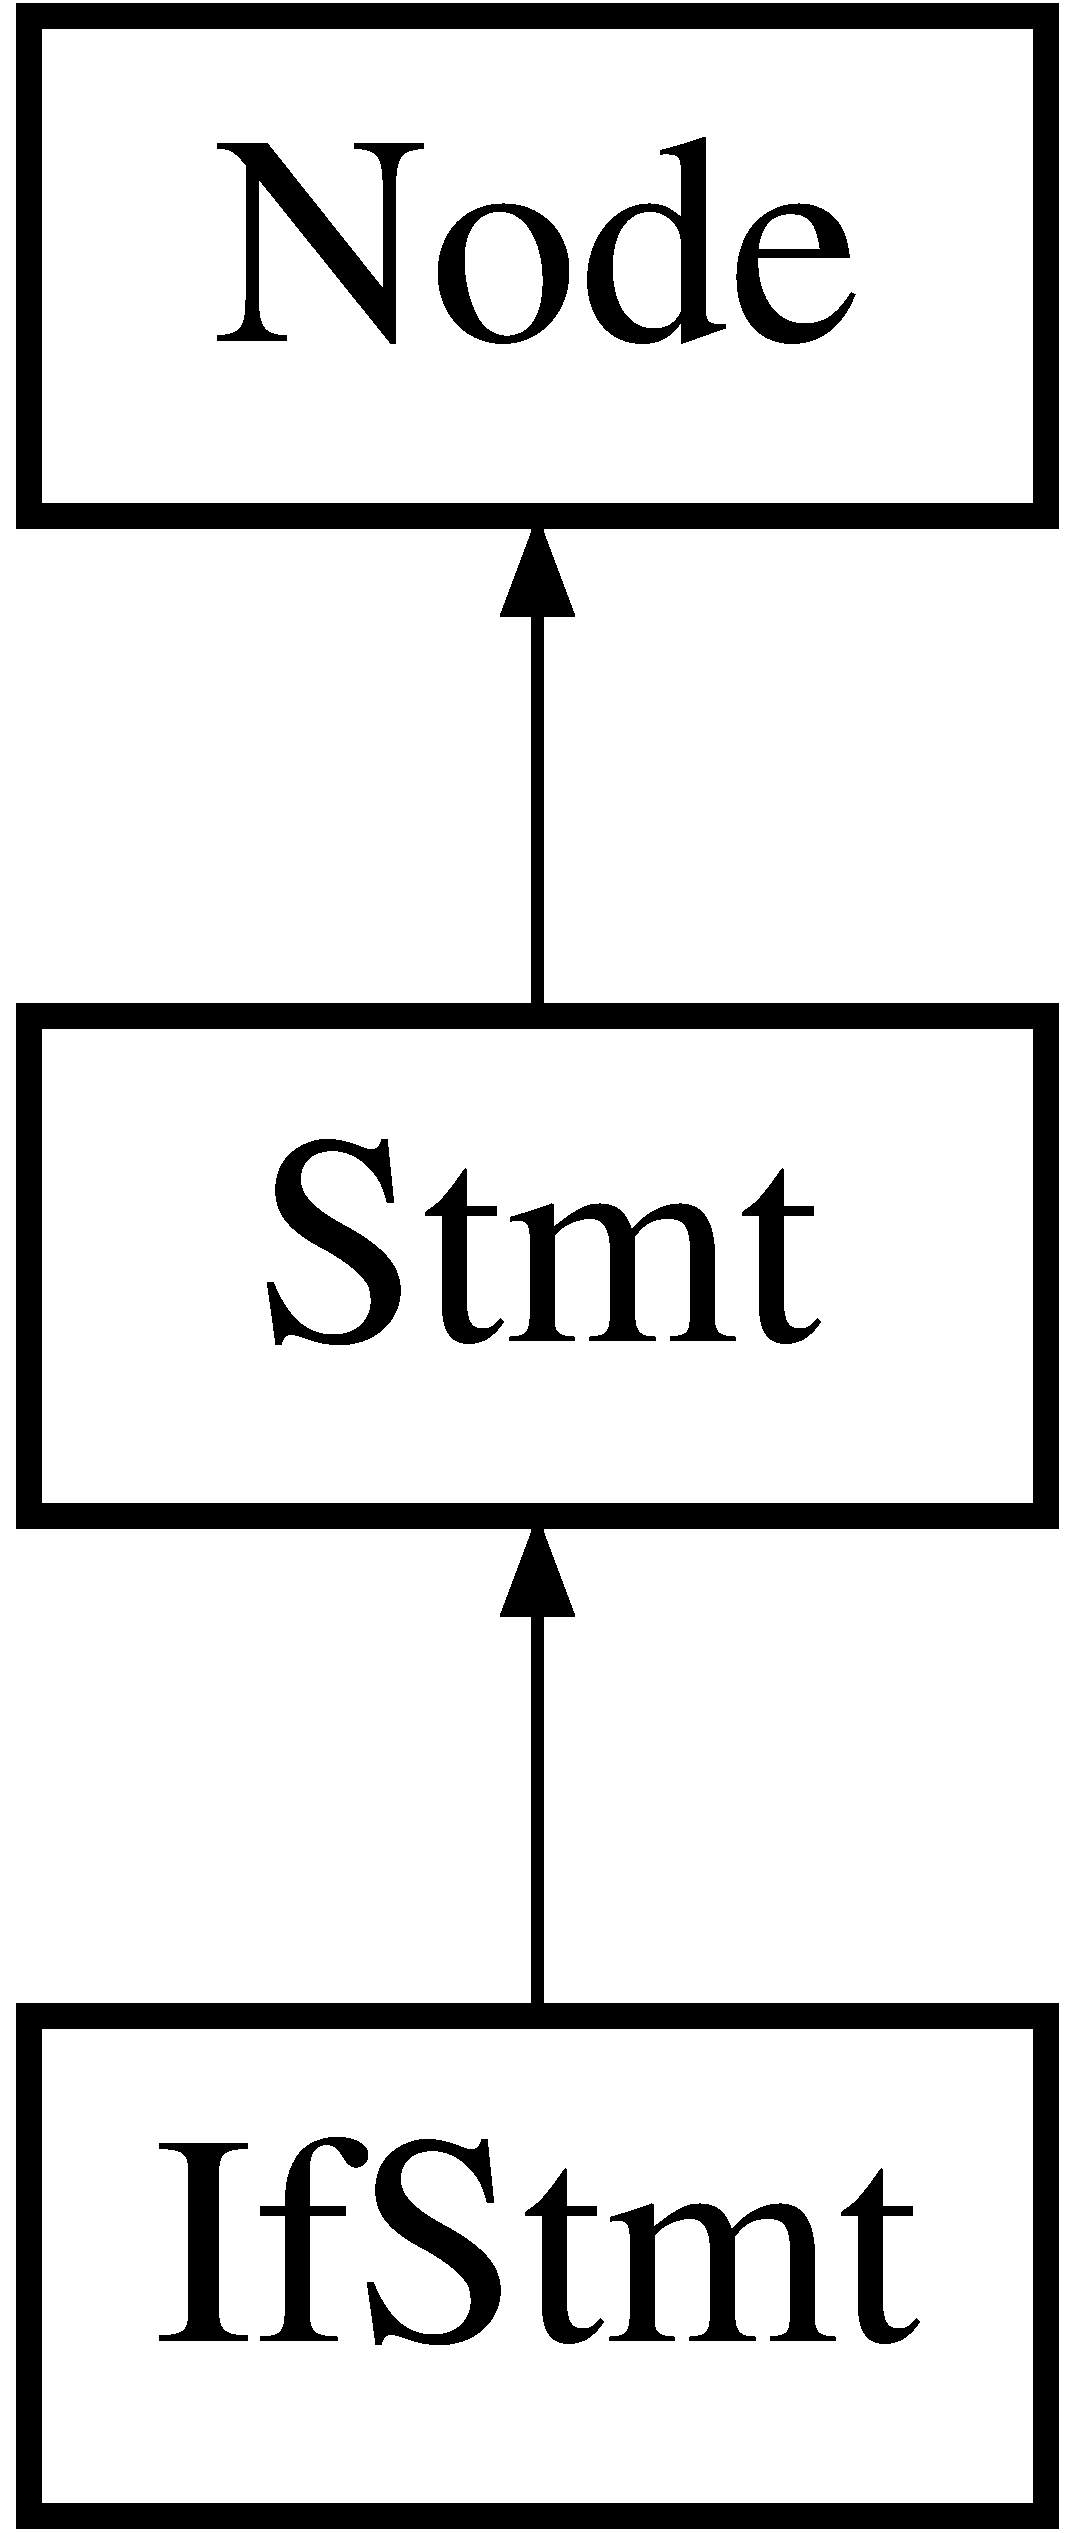
\includegraphics[height=3.000000cm]{classIfStmt}
\end{center}
\end{figure}
\subsection*{Public Member Functions}
\begin{DoxyCompactItemize}
\item 
\hypertarget{classIfStmt_aa80ac539cb4b0f81f85179bd0b8a59e4}{\hyperlink{classIfStmt_aa80ac539cb4b0f81f85179bd0b8a59e4}{If\-Stmt} (\hyperlink{classExpr}{Expr} $\ast$\-\_\-expr, \hyperlink{classStmt}{Stmt} $\ast$\-\_\-stmt)}\label{classIfStmt_aa80ac539cb4b0f81f85179bd0b8a59e4}

\begin{DoxyCompactList}\small\item\em Constructor for \hyperlink{classIfStmt}{If\-Stmt} node. \end{DoxyCompactList}\item 
\hypertarget{classIfStmt_a615e8785edb068f24e19f3ce7863f2ce}{std\-::string \hyperlink{classIfStmt_a615e8785edb068f24e19f3ce7863f2ce}{unparse} ()}\label{classIfStmt_a615e8785edb068f24e19f3ce7863f2ce}

\begin{DoxyCompactList}\small\item\em 'if' '(' \hyperlink{classExpr}{Expr} ')' \hyperlink{classStmt}{Stmt} \end{DoxyCompactList}\end{DoxyCompactItemize}


The documentation for this class was generated from the following files\-:\begin{DoxyCompactItemize}
\item 
A\-S\-T.\-h\item 
A\-S\-T.\-cpp\end{DoxyCompactItemize}

\hypertarget{classIfToken}{\section{If\-Token Class Reference}
\label{classIfToken}\index{If\-Token@{If\-Token}}
}
Inheritance diagram for If\-Token\-:\begin{figure}[H]
\begin{center}
\leavevmode
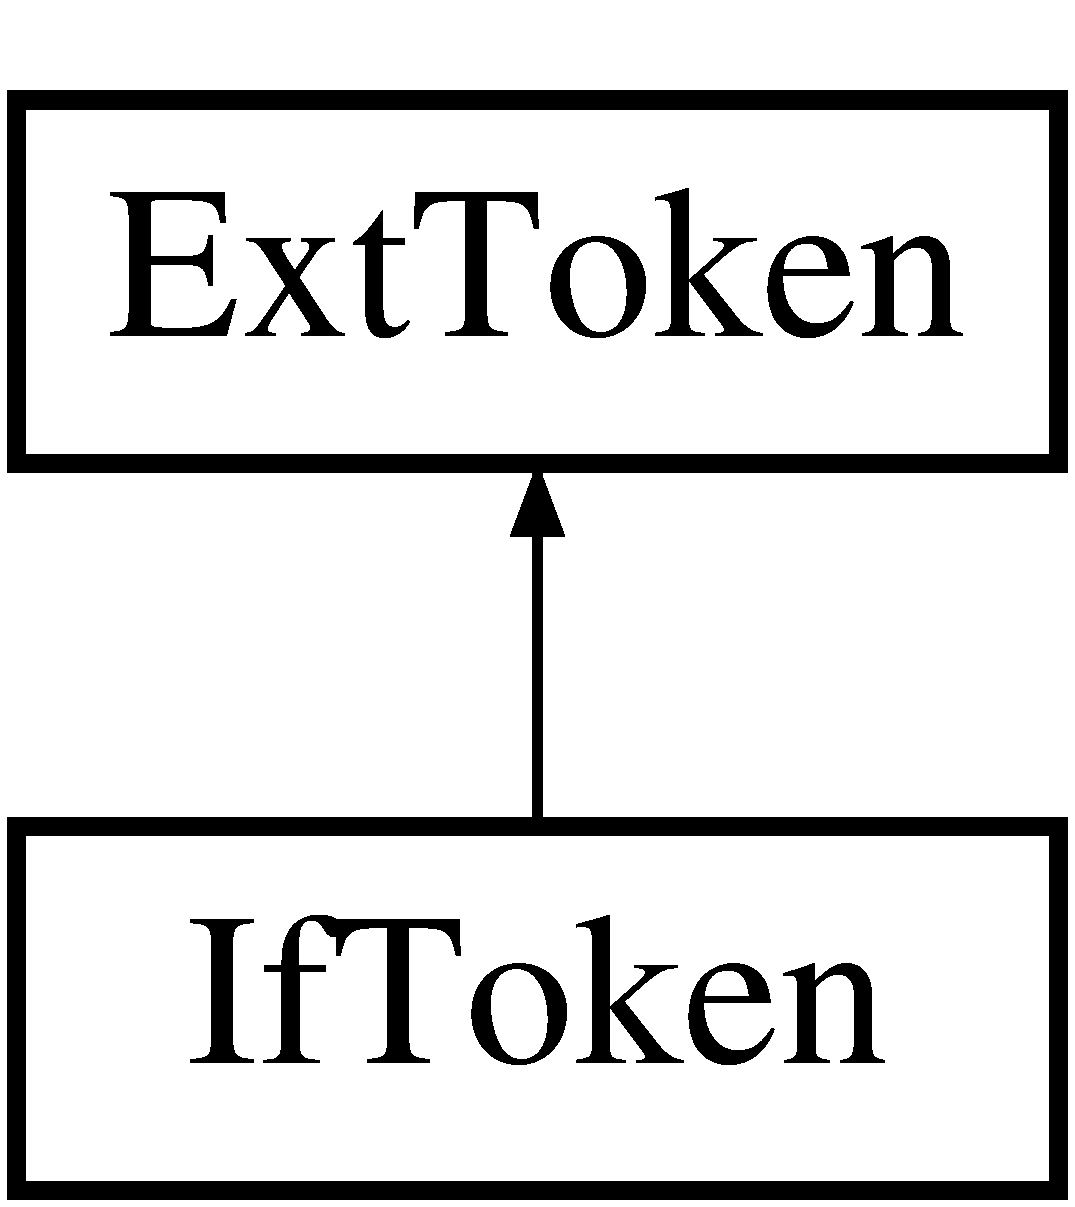
\includegraphics[height=2.000000cm]{classIfToken}
\end{center}
\end{figure}
\subsection*{Public Member Functions}
\begin{DoxyCompactItemize}
\item 
\hypertarget{classIfToken_a607028595b06b8a950000ba3e82329db}{{\bfseries If\-Token} (\hyperlink{classParser}{Parser} $\ast$p, \hyperlink{classToken}{Token} $\ast$t)}\label{classIfToken_a607028595b06b8a950000ba3e82329db}

\item 
\hypertarget{classIfToken_add06bd79ce755fd5503f78e507109e52}{\hyperlink{classParseResult}{Parse\-Result} {\bfseries nud} ()}\label{classIfToken_add06bd79ce755fd5503f78e507109e52}

\item 
\hypertarget{classIfToken_aad226162c5649920c13c2a9e9e7a3617}{std\-::string {\bfseries description} ()}\label{classIfToken_aad226162c5649920c13c2a9e9e7a3617}

\item 
\hypertarget{classIfToken_abfd39ff4c4818d382bf0b97fd097c478}{int {\bfseries lbp} ()}\label{classIfToken_abfd39ff4c4818d382bf0b97fd097c478}

\end{DoxyCompactItemize}
\subsection*{Additional Inherited Members}


The documentation for this class was generated from the following file\-:\begin{DoxyCompactItemize}
\item 
ext\-Token.\-h\end{DoxyCompactItemize}

\hypertarget{classIntConstToken}{\section{Int\-Const\-Token Class Reference}
\label{classIntConstToken}\index{Int\-Const\-Token@{Int\-Const\-Token}}
}
Inheritance diagram for Int\-Const\-Token\-:\begin{figure}[H]
\begin{center}
\leavevmode
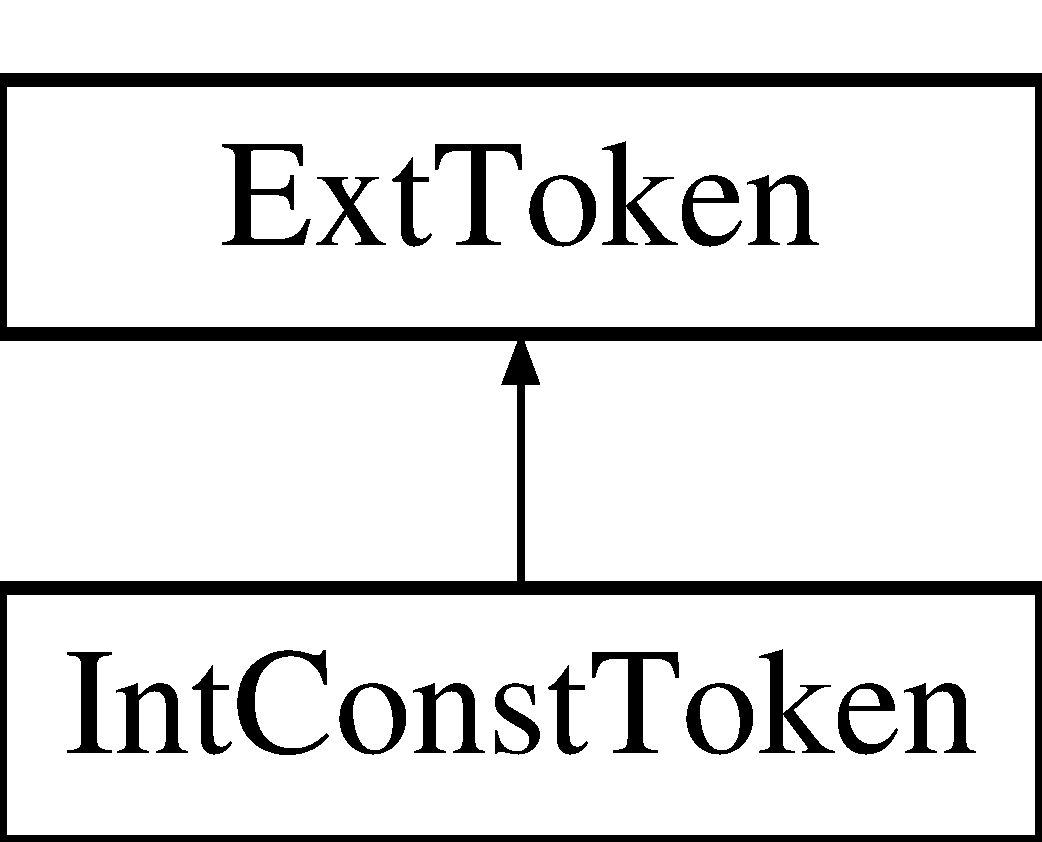
\includegraphics[height=2.000000cm]{classIntConstToken}
\end{center}
\end{figure}
\subsection*{Public Member Functions}
\begin{DoxyCompactItemize}
\item 
\hypertarget{classIntConstToken_a14c6bf0af5a915969b4fef1758067af3}{{\bfseries Int\-Const\-Token} (\hyperlink{classParser}{Parser} $\ast$p, \hyperlink{classToken}{Token} $\ast$t)}\label{classIntConstToken_a14c6bf0af5a915969b4fef1758067af3}

\item 
\hypertarget{classIntConstToken_ae1f720d6006c47e145cae7879d09c708}{\hyperlink{classParseResult}{Parse\-Result} {\bfseries nud} ()}\label{classIntConstToken_ae1f720d6006c47e145cae7879d09c708}

\item 
\hypertarget{classIntConstToken_a98191508d849878d40800e447a0f1892}{std\-::string {\bfseries description} ()}\label{classIntConstToken_a98191508d849878d40800e447a0f1892}

\end{DoxyCompactItemize}
\subsection*{Additional Inherited Members}


The documentation for this class was generated from the following file\-:\begin{DoxyCompactItemize}
\item 
ext\-Token.\-h\end{DoxyCompactItemize}

\hypertarget{classKwdDecl}{\section{Kwd\-Decl Class Reference}
\label{classKwdDecl}\index{Kwd\-Decl@{Kwd\-Decl}}
}
Inheritance diagram for Kwd\-Decl\-:\begin{figure}[H]
\begin{center}
\leavevmode
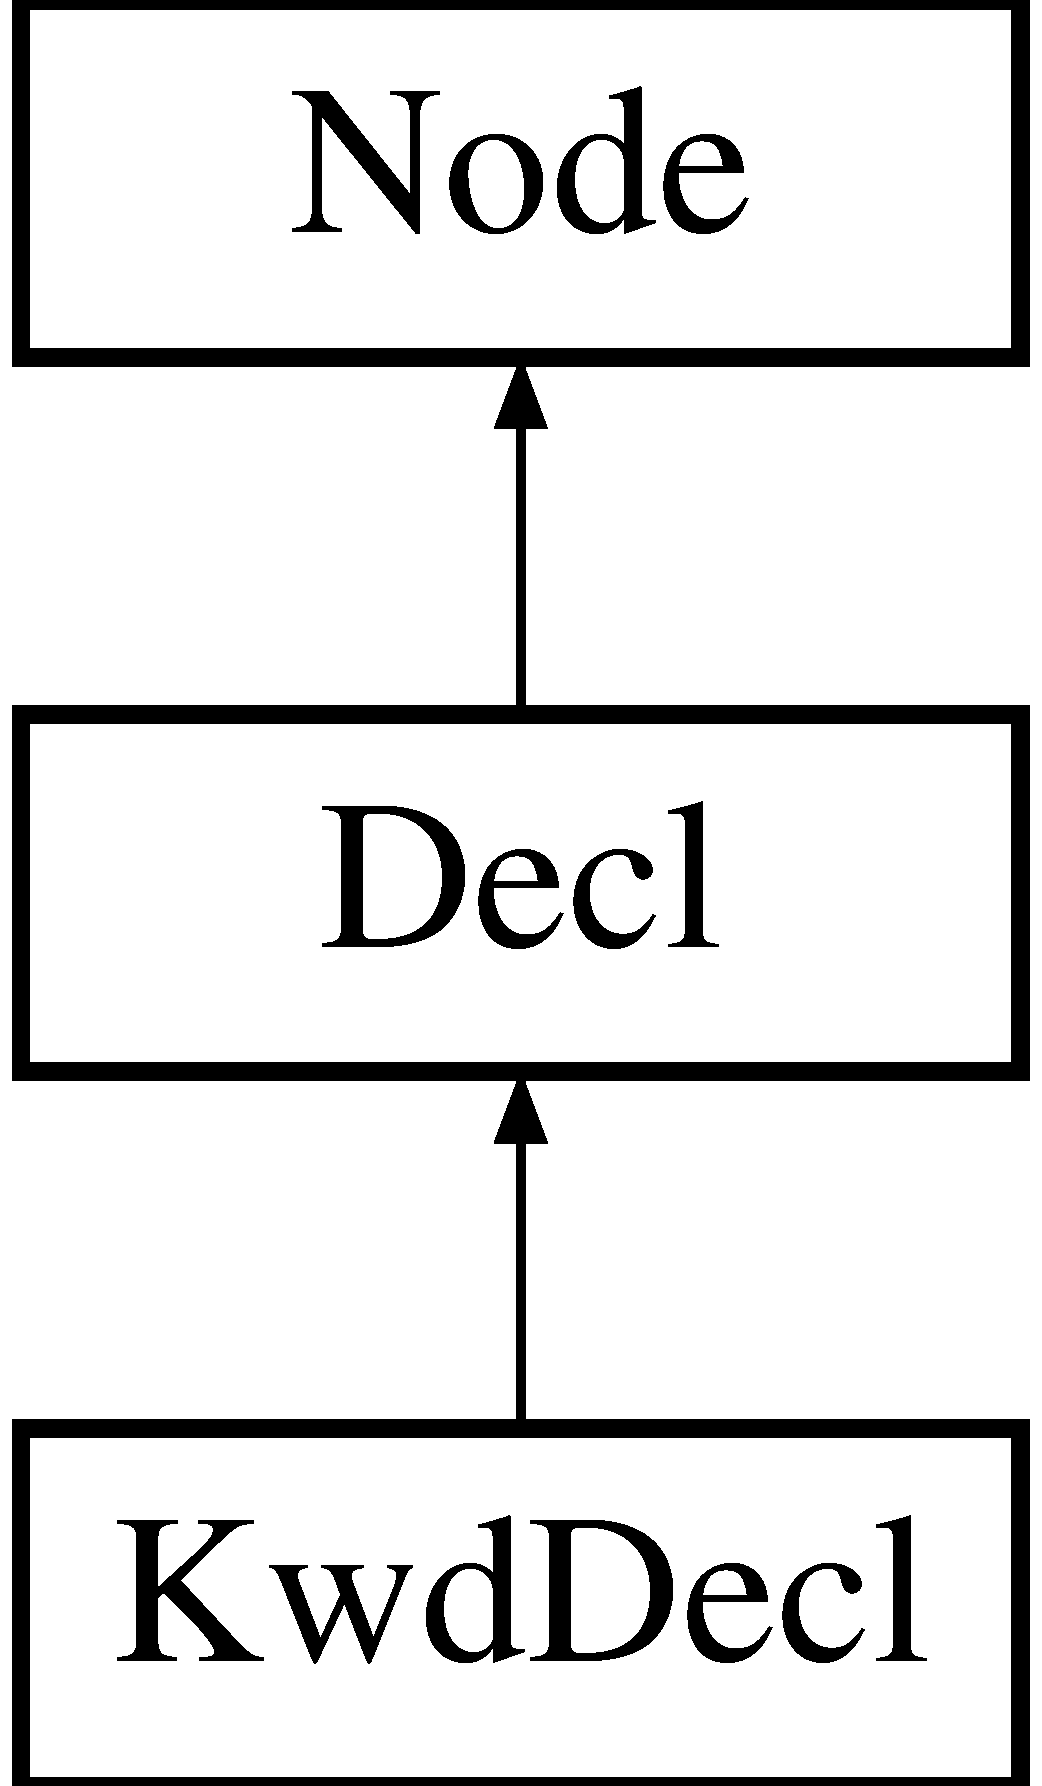
\includegraphics[height=3.000000cm]{classKwdDecl}
\end{center}
\end{figure}
\subsection*{Public Member Functions}
\begin{DoxyCompactItemize}
\item 
\hypertarget{classKwdDecl_a548853ecdec4124e22ab227e6ac96f43}{\hyperlink{classKwdDecl_a548853ecdec4124e22ab227e6ac96f43}{Kwd\-Decl} (std\-::string \-\_\-kwd, std\-::string \-\_\-varname)}\label{classKwdDecl_a548853ecdec4124e22ab227e6ac96f43}

\begin{DoxyCompactList}\small\item\em Constructor for Standard\-Decl node. \end{DoxyCompactList}\item 
\hypertarget{classKwdDecl_ac5f258785ee2a869413772b32c627973}{std\-::string \hyperlink{classKwdDecl_ac5f258785ee2a869413772b32c627973}{unparse} ()}\label{classKwdDecl_ac5f258785ee2a869413772b32c627973}

\begin{DoxyCompactList}\small\item\em 'type' var\-Name ';' \end{DoxyCompactList}\end{DoxyCompactItemize}


The documentation for this class was generated from the following files\-:\begin{DoxyCompactItemize}
\item 
A\-S\-T.\-h\item 
A\-S\-T.\-cpp\end{DoxyCompactItemize}

\hypertarget{classLeftParenToken}{\section{Left\-Paren\-Token Class Reference}
\label{classLeftParenToken}\index{Left\-Paren\-Token@{Left\-Paren\-Token}}
}
Inheritance diagram for Left\-Paren\-Token\-:\begin{figure}[H]
\begin{center}
\leavevmode
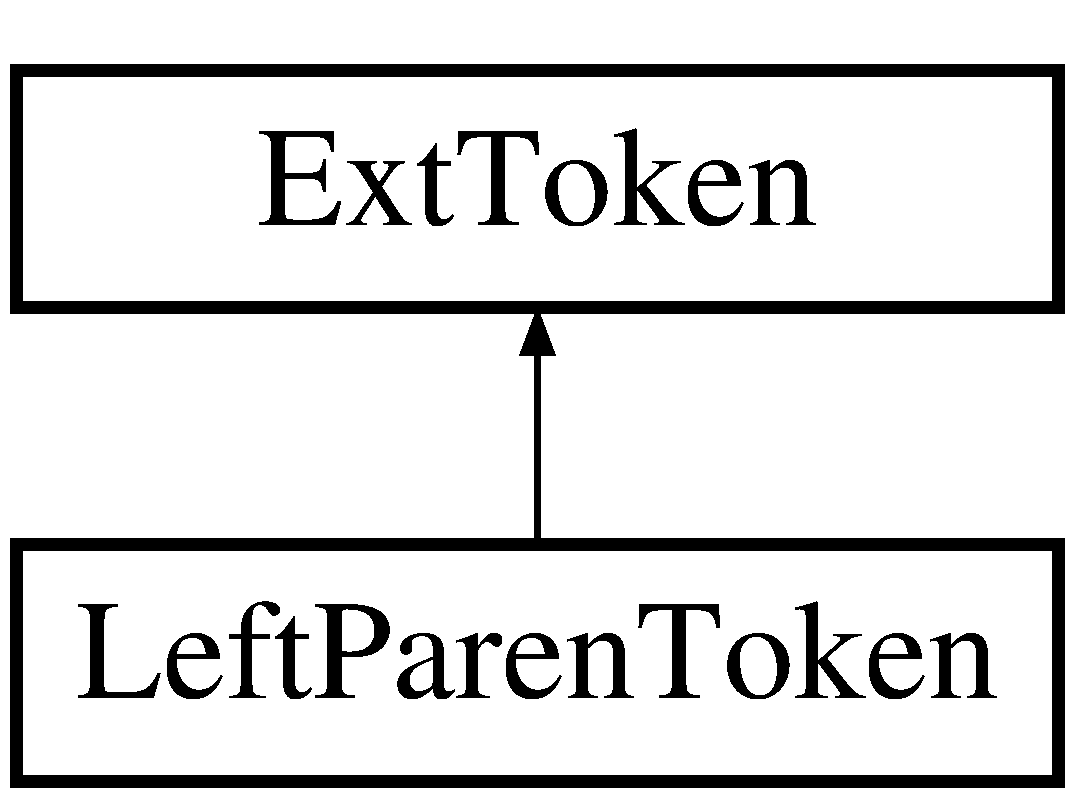
\includegraphics[height=2.000000cm]{classLeftParenToken}
\end{center}
\end{figure}
\subsection*{Public Member Functions}
\begin{DoxyCompactItemize}
\item 
\hypertarget{classLeftParenToken_aecdc6faf48a1a7192ec55712f0264cba}{{\bfseries Left\-Paren\-Token} (\hyperlink{classParser}{Parser} $\ast$p, \hyperlink{classToken}{Token} $\ast$t)}\label{classLeftParenToken_aecdc6faf48a1a7192ec55712f0264cba}

\item 
\hypertarget{classLeftParenToken_a3cb3ae9ab2647e5534c85529d314f08b}{\hyperlink{classParseResult}{Parse\-Result} {\bfseries nud} ()}\label{classLeftParenToken_a3cb3ae9ab2647e5534c85529d314f08b}

\item 
\hypertarget{classLeftParenToken_a2df35684bd2081c3bdfe2357946917bc}{std\-::string {\bfseries description} ()}\label{classLeftParenToken_a2df35684bd2081c3bdfe2357946917bc}

\item 
\hypertarget{classLeftParenToken_afa1b94645278f097bb097d3b24445d14}{int {\bfseries lbp} ()}\label{classLeftParenToken_afa1b94645278f097bb097d3b24445d14}

\end{DoxyCompactItemize}
\subsection*{Additional Inherited Members}


The documentation for this class was generated from the following file\-:\begin{DoxyCompactItemize}
\item 
ext\-Token.\-h\end{DoxyCompactItemize}

\hypertarget{classLetExpr}{\section{Let\-Expr Class Reference}
\label{classLetExpr}\index{Let\-Expr@{Let\-Expr}}
}
Inheritance diagram for Let\-Expr\-:\begin{figure}[H]
\begin{center}
\leavevmode
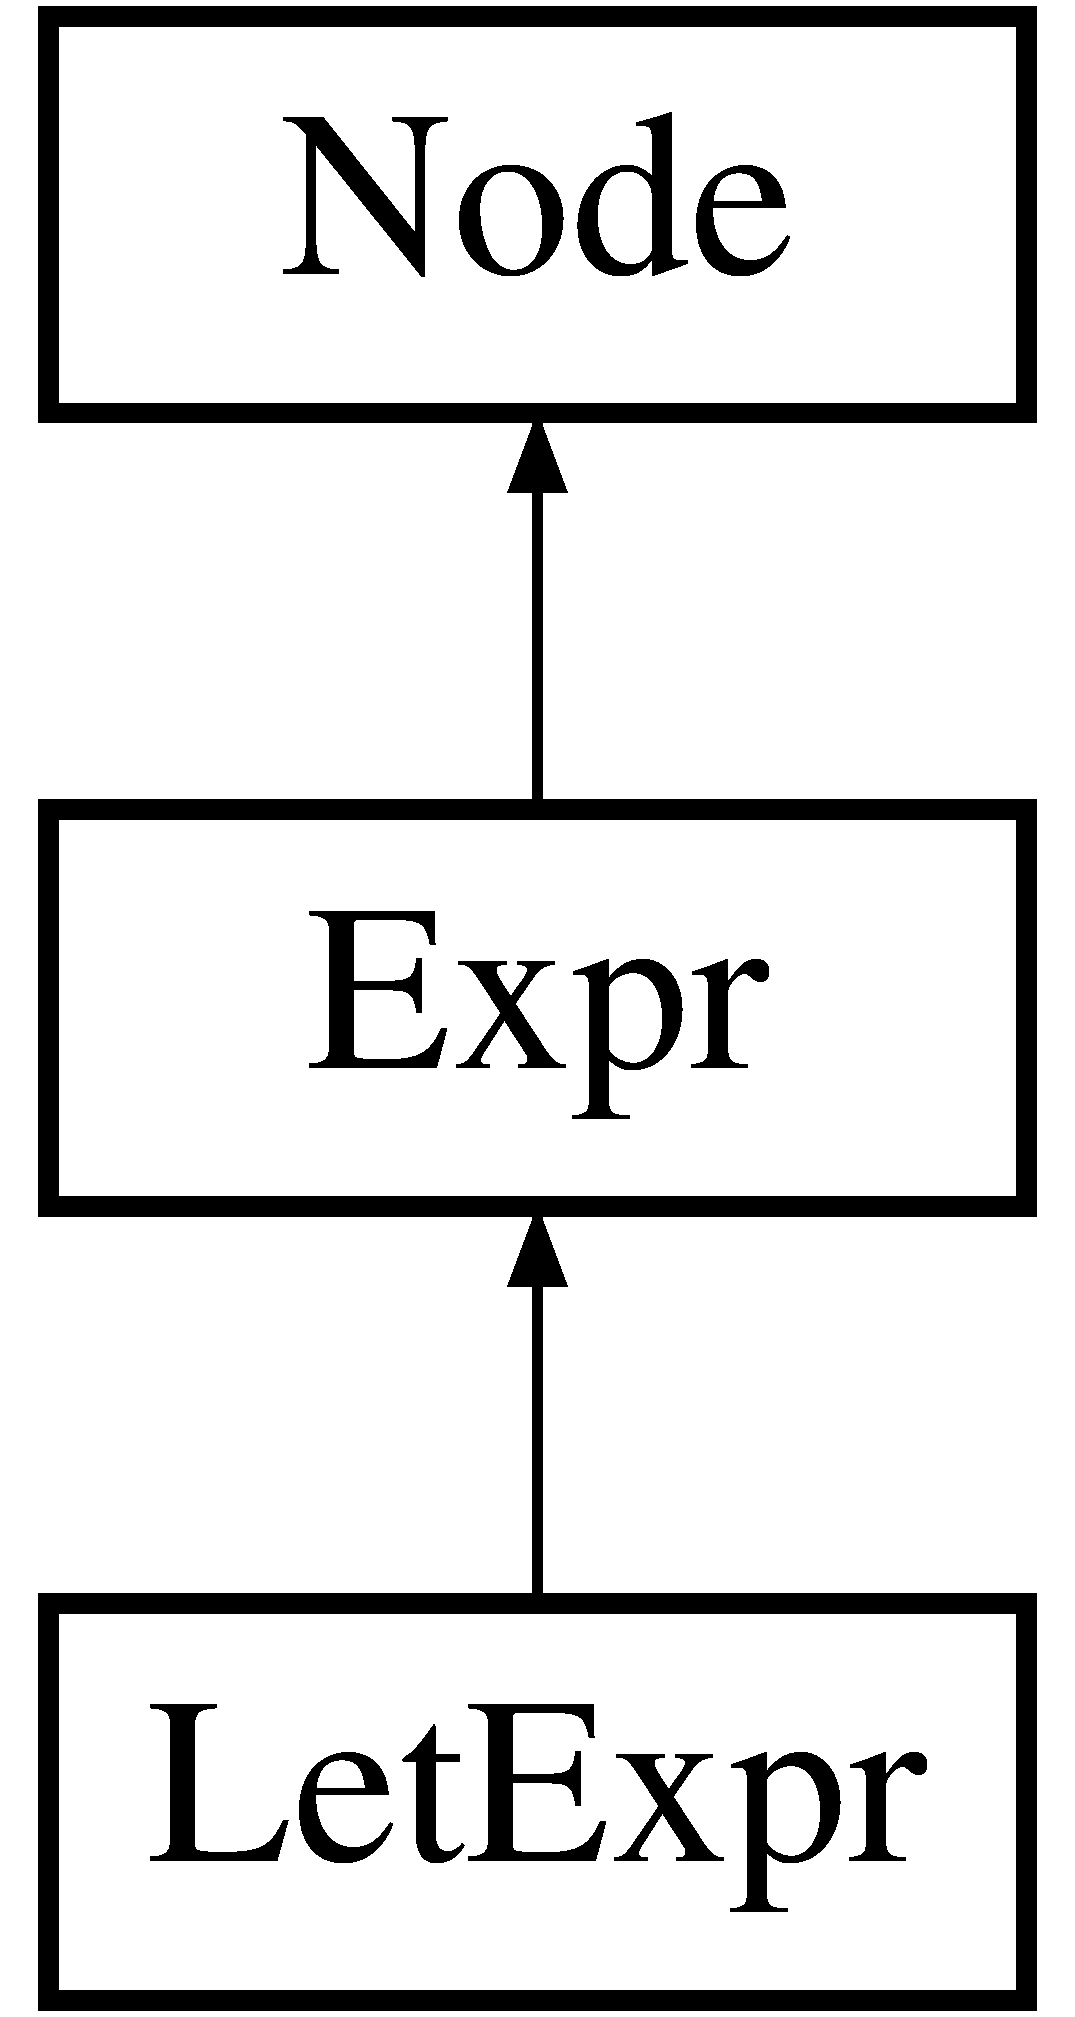
\includegraphics[height=3.000000cm]{classLetExpr}
\end{center}
\end{figure}
\subsection*{Public Member Functions}
\begin{DoxyCompactItemize}
\item 
\hypertarget{classLetExpr_a9cb6116997c5d803d1872716c05937e1}{\hyperlink{classLetExpr_a9cb6116997c5d803d1872716c05937e1}{Let\-Expr} (\hyperlink{classStmts}{Stmts} $\ast$\-\_\-stmts, \hyperlink{classExpr}{Expr} $\ast$\-\_\-expr)}\label{classLetExpr_a9cb6116997c5d803d1872716c05937e1}

\begin{DoxyCompactList}\small\item\em Constructor for \hyperlink{classLetExpr}{Let\-Expr} node. \end{DoxyCompactList}\item 
\hypertarget{classLetExpr_a47e9e62ebec3114d50c127223fff126b}{std\-::string \hyperlink{classLetExpr_a47e9e62ebec3114d50c127223fff126b}{unparse} ()}\label{classLetExpr_a47e9e62ebec3114d50c127223fff126b}

\begin{DoxyCompactList}\small\item\em 'let' \hyperlink{classStmts}{Stmts} 'in' \hyperlink{classExpr}{Expr} 'end' \end{DoxyCompactList}\end{DoxyCompactItemize}


The documentation for this class was generated from the following files\-:\begin{DoxyCompactItemize}
\item 
A\-S\-T.\-h\item 
A\-S\-T.\-cpp\end{DoxyCompactItemize}

\hypertarget{classLetToken}{\section{Let\-Token Class Reference}
\label{classLetToken}\index{Let\-Token@{Let\-Token}}
}
Inheritance diagram for Let\-Token\-:\begin{figure}[H]
\begin{center}
\leavevmode
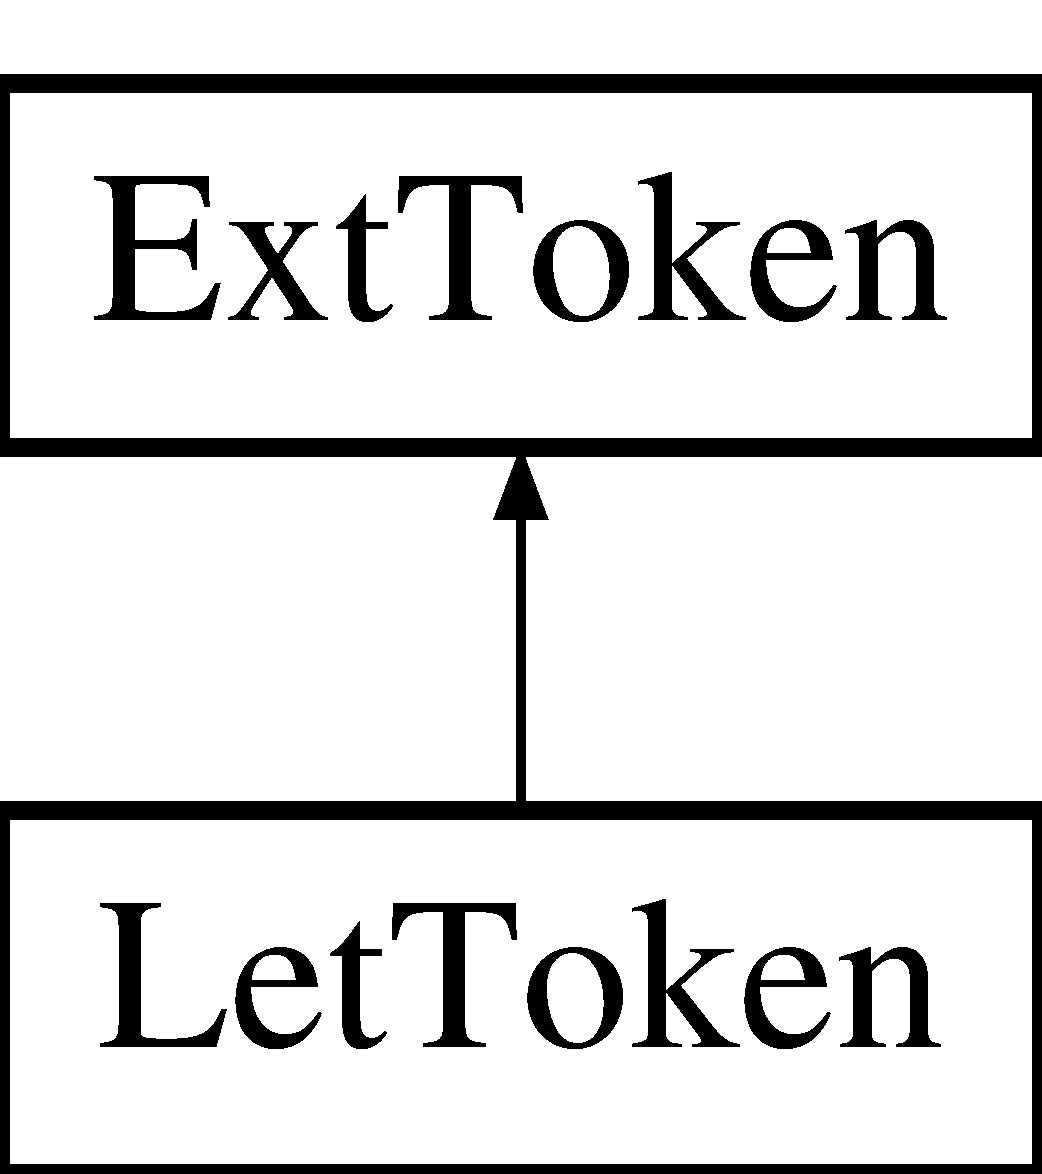
\includegraphics[height=2.000000cm]{classLetToken}
\end{center}
\end{figure}
\subsection*{Public Member Functions}
\begin{DoxyCompactItemize}
\item 
\hypertarget{classLetToken_a94651a82207e47cd2c1066a58cb1fe08}{{\bfseries Let\-Token} (\hyperlink{classParser}{Parser} $\ast$p, \hyperlink{classToken}{Token} $\ast$t)}\label{classLetToken_a94651a82207e47cd2c1066a58cb1fe08}

\item 
\hypertarget{classLetToken_a14df948cdf775bde8392bf58d53b91f3}{\hyperlink{classParseResult}{Parse\-Result} {\bfseries nud} ()}\label{classLetToken_a14df948cdf775bde8392bf58d53b91f3}

\item 
\hypertarget{classLetToken_a2c5ba0489774bf6468a26f4e19d7fab4}{std\-::string {\bfseries description} ()}\label{classLetToken_a2c5ba0489774bf6468a26f4e19d7fab4}

\item 
\hypertarget{classLetToken_a2a5ab5bc5897340513480c162bb2b065}{int {\bfseries lbp} ()}\label{classLetToken_a2a5ab5bc5897340513480c162bb2b065}

\end{DoxyCompactItemize}
\subsection*{Additional Inherited Members}


The documentation for this class was generated from the following file\-:\begin{DoxyCompactItemize}
\item 
ext\-Token.\-h\end{DoxyCompactItemize}

\hypertarget{classMatrixDecl}{\section{Matrix\-Decl Class Reference}
\label{classMatrixDecl}\index{Matrix\-Decl@{Matrix\-Decl}}
}
Inheritance diagram for Matrix\-Decl\-:\begin{figure}[H]
\begin{center}
\leavevmode
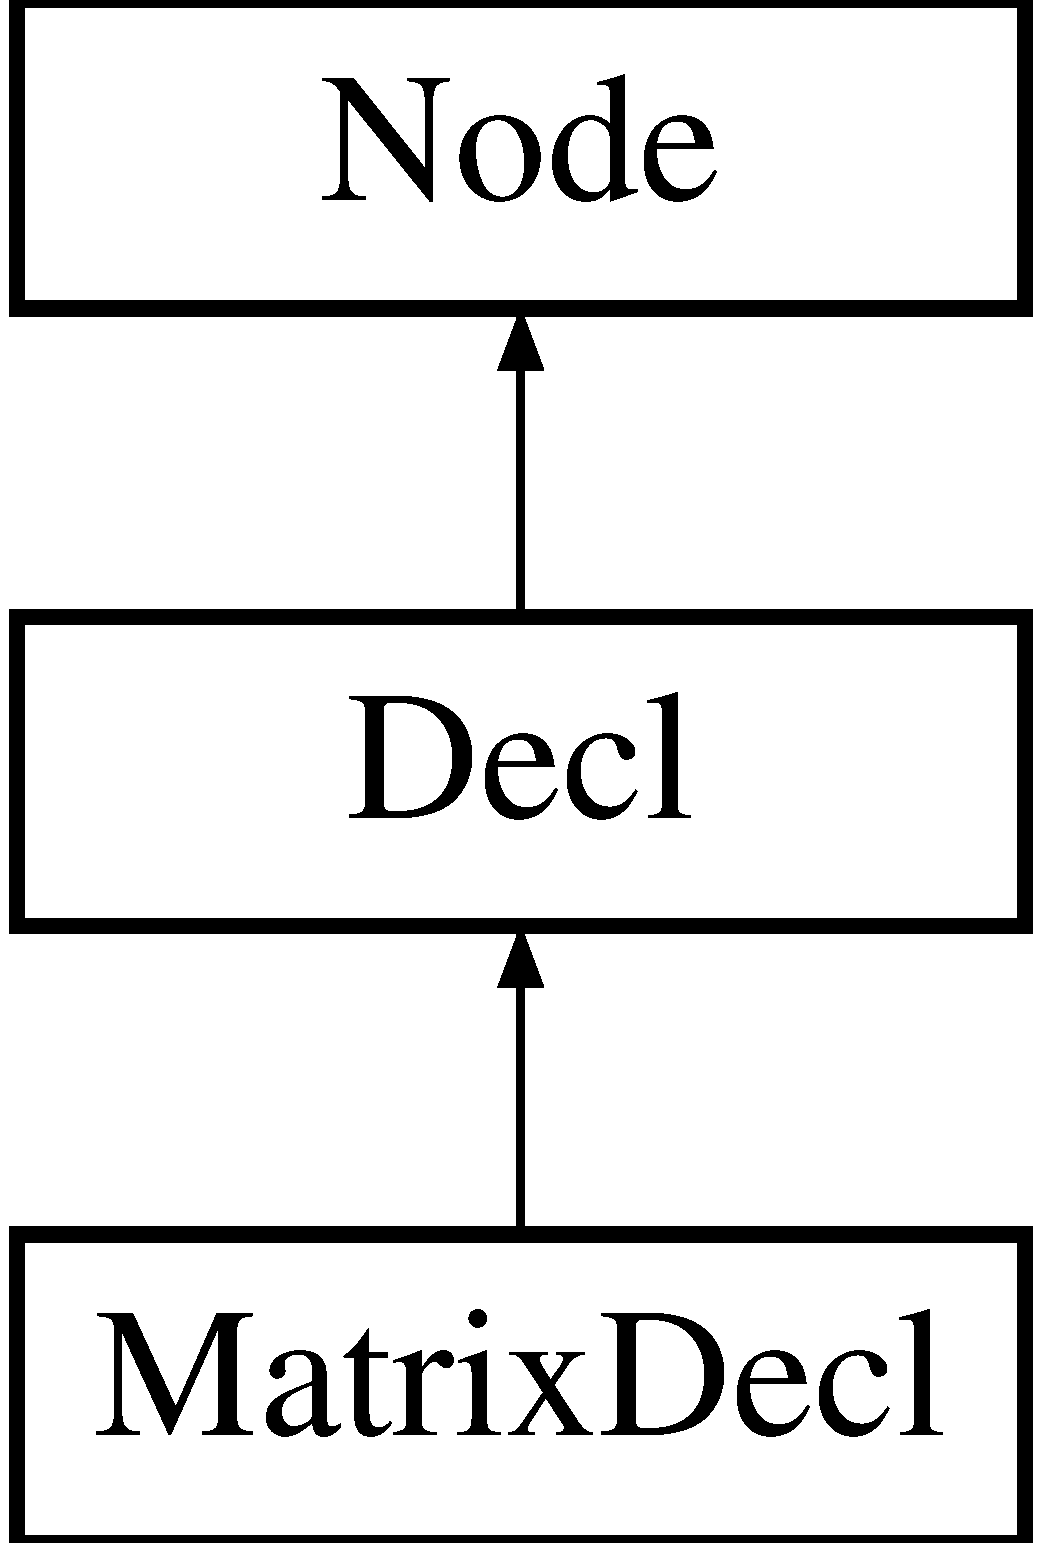
\includegraphics[height=3.000000cm]{classMatrixDecl}
\end{center}
\end{figure}
\subsection*{Public Member Functions}
\begin{DoxyCompactItemize}
\item 
\hypertarget{classMatrixDecl_a805f800309bafcfa1f5b80c3621f142e}{\hyperlink{classMatrixDecl_a805f800309bafcfa1f5b80c3621f142e}{Matrix\-Decl} (std\-::string \-\_\-varname, \hyperlink{classExpr}{Expr} $\ast$\-\_\-expr)}\label{classMatrixDecl_a805f800309bafcfa1f5b80c3621f142e}

\begin{DoxyCompactList}\small\item\em Constructor for \hyperlink{classMatrixDecl}{Matrix\-Decl} node. \end{DoxyCompactList}\item 
\hypertarget{classMatrixDecl_a86609ed608879ec9a72a2a96ea924c89}{std\-::string \hyperlink{classMatrixDecl_a86609ed608879ec9a72a2a96ea924c89}{unparse} ()}\label{classMatrixDecl_a86609ed608879ec9a72a2a96ea924c89}

\begin{DoxyCompactList}\small\item\em 'Matrix' var\-Name '=' \hyperlink{classExpr}{Expr} ';' \end{DoxyCompactList}\end{DoxyCompactItemize}


The documentation for this class was generated from the following files\-:\begin{DoxyCompactItemize}
\item 
A\-S\-T.\-h\item 
A\-S\-T.\-cpp\end{DoxyCompactItemize}

\hypertarget{classMatrixRefExpr}{\section{Matrix\-Ref\-Expr Class Reference}
\label{classMatrixRefExpr}\index{Matrix\-Ref\-Expr@{Matrix\-Ref\-Expr}}
}
Inheritance diagram for Matrix\-Ref\-Expr\-:\begin{figure}[H]
\begin{center}
\leavevmode
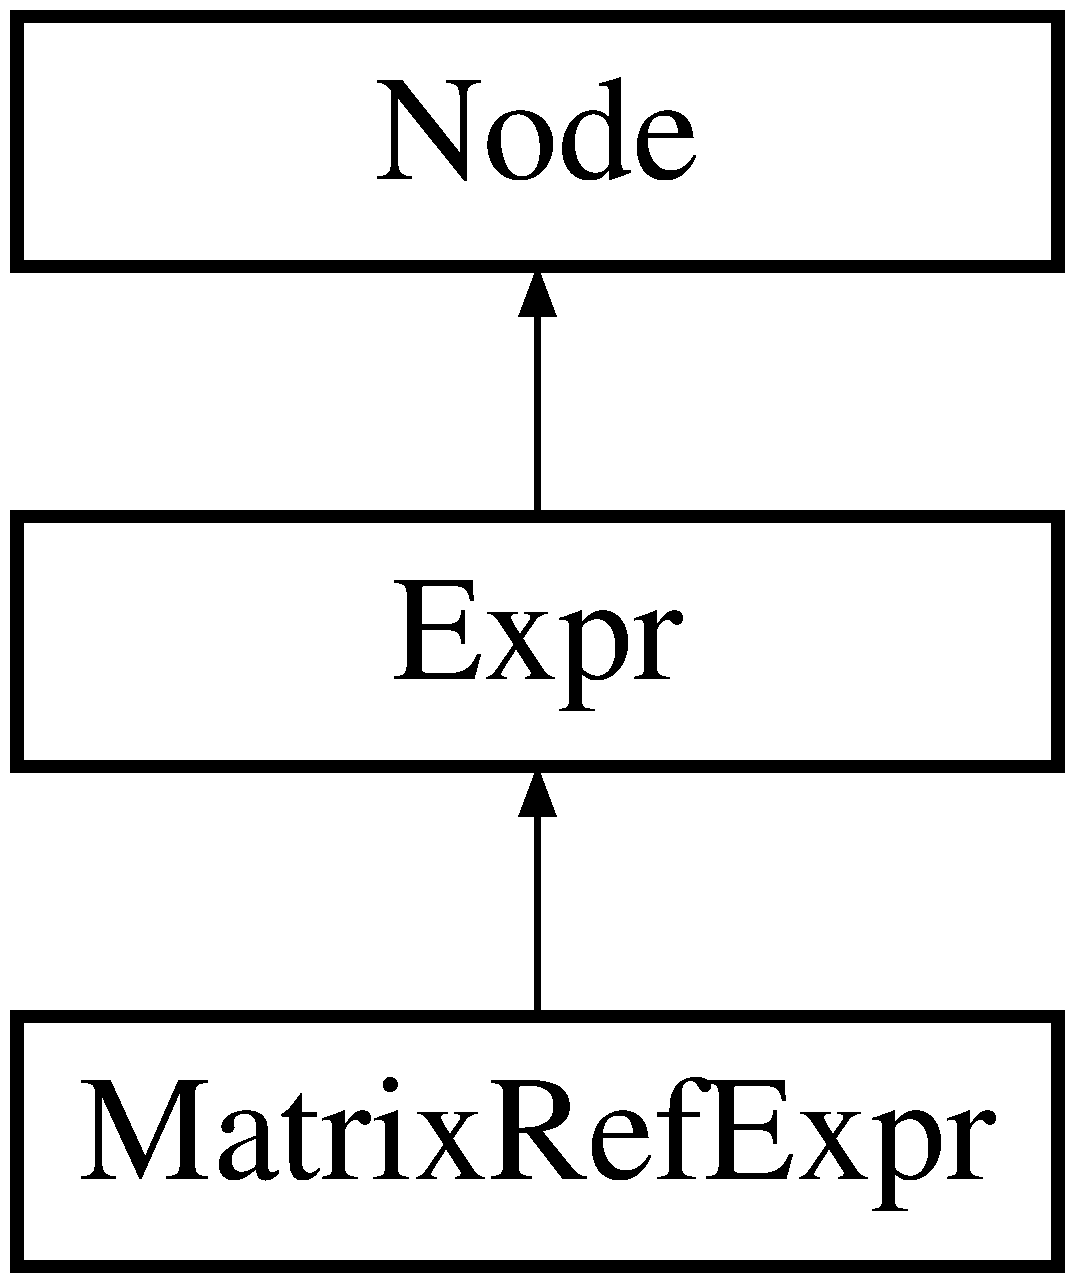
\includegraphics[height=3.000000cm]{classMatrixRefExpr}
\end{center}
\end{figure}
\subsection*{Public Member Functions}
\begin{DoxyCompactItemize}
\item 
\hypertarget{classMatrixRefExpr_acb6aba5d43984e83882d75f0dbcf5998}{\hyperlink{classMatrixRefExpr_acb6aba5d43984e83882d75f0dbcf5998}{Matrix\-Ref\-Expr} (std\-::string \-\_\-varname, \hyperlink{classExpr}{Expr} $\ast$\-\_\-expr1, \hyperlink{classExpr}{Expr} $\ast$\-\_\-expr2)}\label{classMatrixRefExpr_acb6aba5d43984e83882d75f0dbcf5998}

\begin{DoxyCompactList}\small\item\em Constructor for \hyperlink{classMatrixRefExpr}{Matrix\-Ref\-Expr} node. \end{DoxyCompactList}\item 
\hypertarget{classMatrixRefExpr_ac1eaeb36db1b33ea1ba6bb639ee93e04}{std\-::string \hyperlink{classMatrixRefExpr_ac1eaeb36db1b33ea1ba6bb639ee93e04}{unparse} ()}\label{classMatrixRefExpr_ac1eaeb36db1b33ea1ba6bb639ee93e04}

\begin{DoxyCompactList}\small\item\em var\-Name '\mbox{[}' \hyperlink{classExpr}{Expr} ',' \hyperlink{classExpr}{Expr} '\mbox{]}' \end{DoxyCompactList}\end{DoxyCompactItemize}


The documentation for this class was generated from the following files\-:\begin{DoxyCompactItemize}
\item 
A\-S\-T.\-h\item 
A\-S\-T.\-cpp\end{DoxyCompactItemize}

\hypertarget{classNestedExpr}{\section{Nested\-Expr Class Reference}
\label{classNestedExpr}\index{Nested\-Expr@{Nested\-Expr}}
}
Inheritance diagram for Nested\-Expr\-:\begin{figure}[H]
\begin{center}
\leavevmode
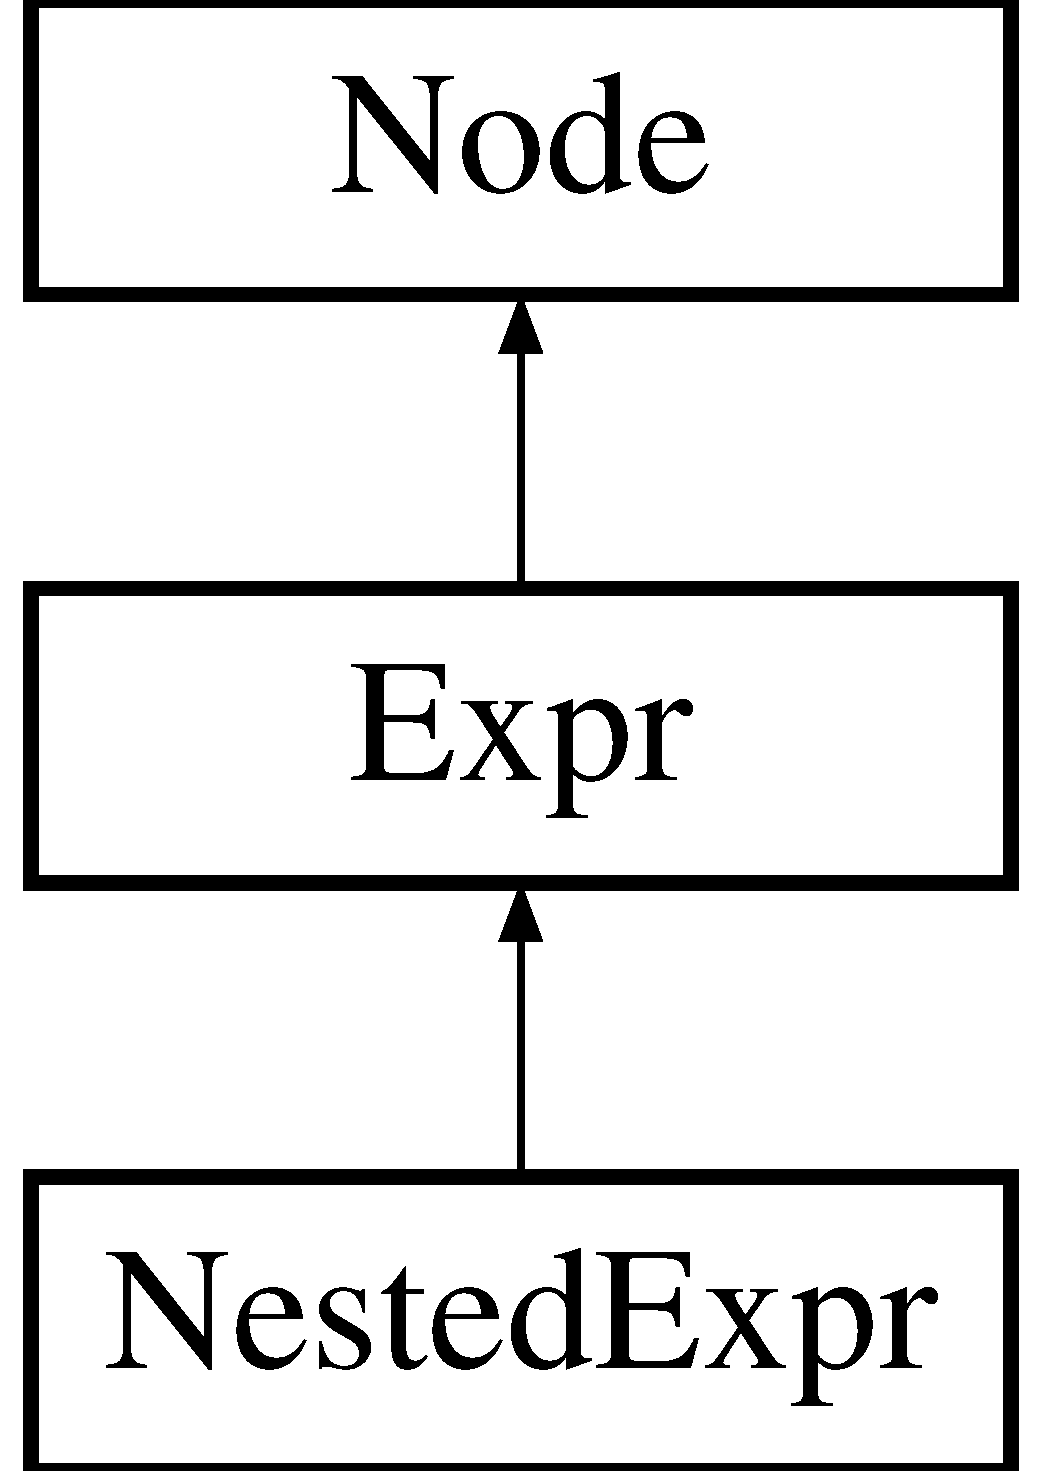
\includegraphics[height=3.000000cm]{classNestedExpr}
\end{center}
\end{figure}
\subsection*{Public Member Functions}
\begin{DoxyCompactItemize}
\item 
\hypertarget{classNestedExpr_a7da30ea4b79ff2c029eaf82e1811f817}{\hyperlink{classNestedExpr_a7da30ea4b79ff2c029eaf82e1811f817}{Nested\-Expr} (\hyperlink{classExpr}{Expr} $\ast$\-\_\-expr)}\label{classNestedExpr_a7da30ea4b79ff2c029eaf82e1811f817}

\begin{DoxyCompactList}\small\item\em Constructor for \hyperlink{classNestedExpr}{Nested\-Expr} node. \end{DoxyCompactList}\item 
\hypertarget{classNestedExpr_a4cf035c9980349fb9dbe6285b3ae4cc9}{std\-::string \hyperlink{classNestedExpr_a4cf035c9980349fb9dbe6285b3ae4cc9}{unparse} ()}\label{classNestedExpr_a4cf035c9980349fb9dbe6285b3ae4cc9}

\begin{DoxyCompactList}\small\item\em '(' \hyperlink{classExpr}{Expr} ')' \end{DoxyCompactList}\end{DoxyCompactItemize}


The documentation for this class was generated from the following files\-:\begin{DoxyCompactItemize}
\item 
A\-S\-T.\-h\item 
A\-S\-T.\-cpp\end{DoxyCompactItemize}

\hypertarget{classNestedOrFunctionCallExpr}{\section{Nested\-Or\-Function\-Call\-Expr Class Reference}
\label{classNestedOrFunctionCallExpr}\index{Nested\-Or\-Function\-Call\-Expr@{Nested\-Or\-Function\-Call\-Expr}}
}
Inheritance diagram for Nested\-Or\-Function\-Call\-Expr\-:\begin{figure}[H]
\begin{center}
\leavevmode
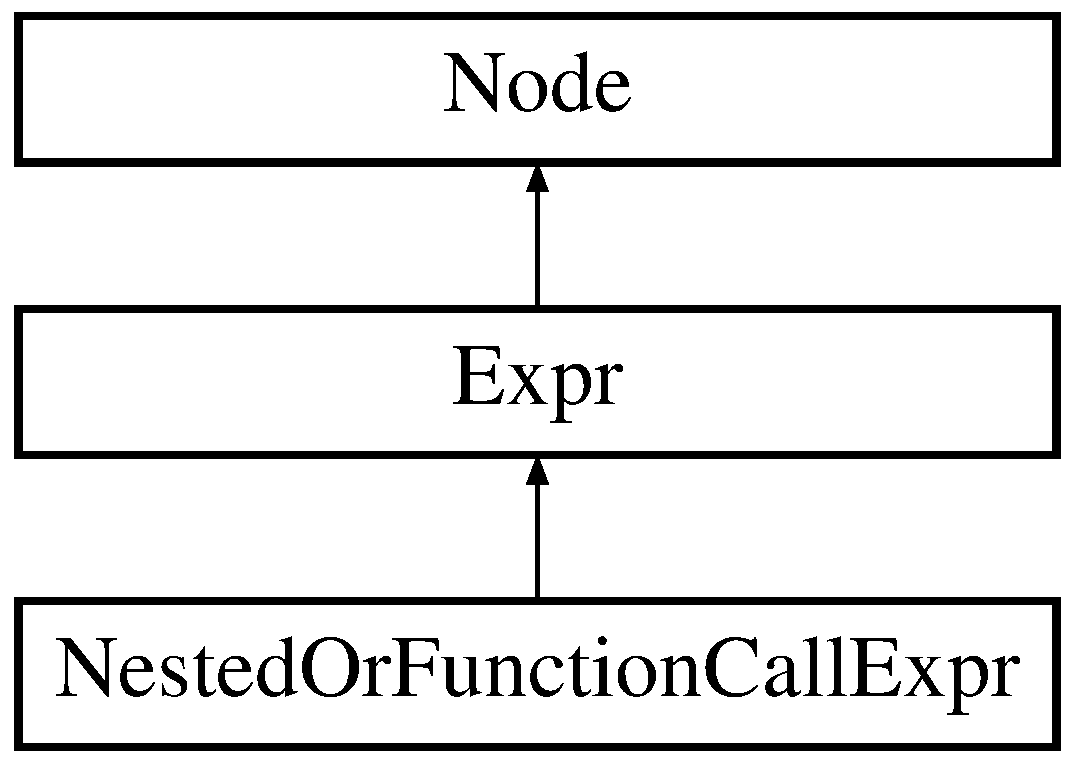
\includegraphics[height=3.000000cm]{classNestedOrFunctionCallExpr}
\end{center}
\end{figure}
\subsection*{Public Member Functions}
\begin{DoxyCompactItemize}
\item 
\hypertarget{classNestedOrFunctionCallExpr_abdf4c721e93d55f3983669df76d6cc24}{\hyperlink{classNestedOrFunctionCallExpr_abdf4c721e93d55f3983669df76d6cc24}{Nested\-Or\-Function\-Call\-Expr} (std\-::string \-\_\-varname, \hyperlink{classExpr}{Expr} $\ast$\-\_\-expr)}\label{classNestedOrFunctionCallExpr_abdf4c721e93d55f3983669df76d6cc24}

\begin{DoxyCompactList}\small\item\em Constructor for \hyperlink{classNestedOrFunctionCallExpr}{Nested\-Or\-Function\-Call\-Expr} node. \end{DoxyCompactList}\item 
\hypertarget{classNestedOrFunctionCallExpr_aac49f863b8cf73a671479b4d414f61bd}{std\-::string \hyperlink{classNestedOrFunctionCallExpr_aac49f863b8cf73a671479b4d414f61bd}{unparse} ()}\label{classNestedOrFunctionCallExpr_aac49f863b8cf73a671479b4d414f61bd}

\begin{DoxyCompactList}\small\item\em Method to unparse. \end{DoxyCompactList}\end{DoxyCompactItemize}


The documentation for this class was generated from the following files\-:\begin{DoxyCompactItemize}
\item 
A\-S\-T.\-h\item 
A\-S\-T.\-cpp\end{DoxyCompactItemize}

\hypertarget{classNode}{\section{Node Class Reference}
\label{classNode}\index{Node@{Node}}
}
Inheritance diagram for Node\-:\begin{figure}[H]
\begin{center}
\leavevmode
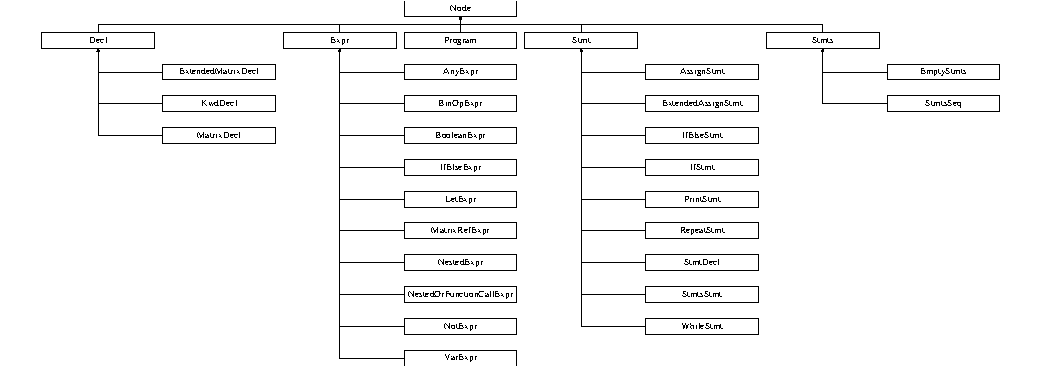
\includegraphics[height=4.912281cm]{classNode}
\end{center}
\end{figure}
\subsection*{Public Member Functions}
\begin{DoxyCompactItemize}
\item 
\hypertarget{classNode_a60ea533e0900961c05e701db70097136}{virtual std\-::string \hyperlink{classNode_a60ea533e0900961c05e701db70097136}{unparse} ()=0}\label{classNode_a60ea533e0900961c05e701db70097136}

\begin{DoxyCompactList}\small\item\em Method to unparse. \end{DoxyCompactList}\end{DoxyCompactItemize}


The documentation for this class was generated from the following file\-:\begin{DoxyCompactItemize}
\item 
A\-S\-T.\-h\end{DoxyCompactItemize}

\hypertarget{classNotExpr}{\section{Not\-Expr Class Reference}
\label{classNotExpr}\index{Not\-Expr@{Not\-Expr}}
}
Inheritance diagram for Not\-Expr\-:\begin{figure}[H]
\begin{center}
\leavevmode
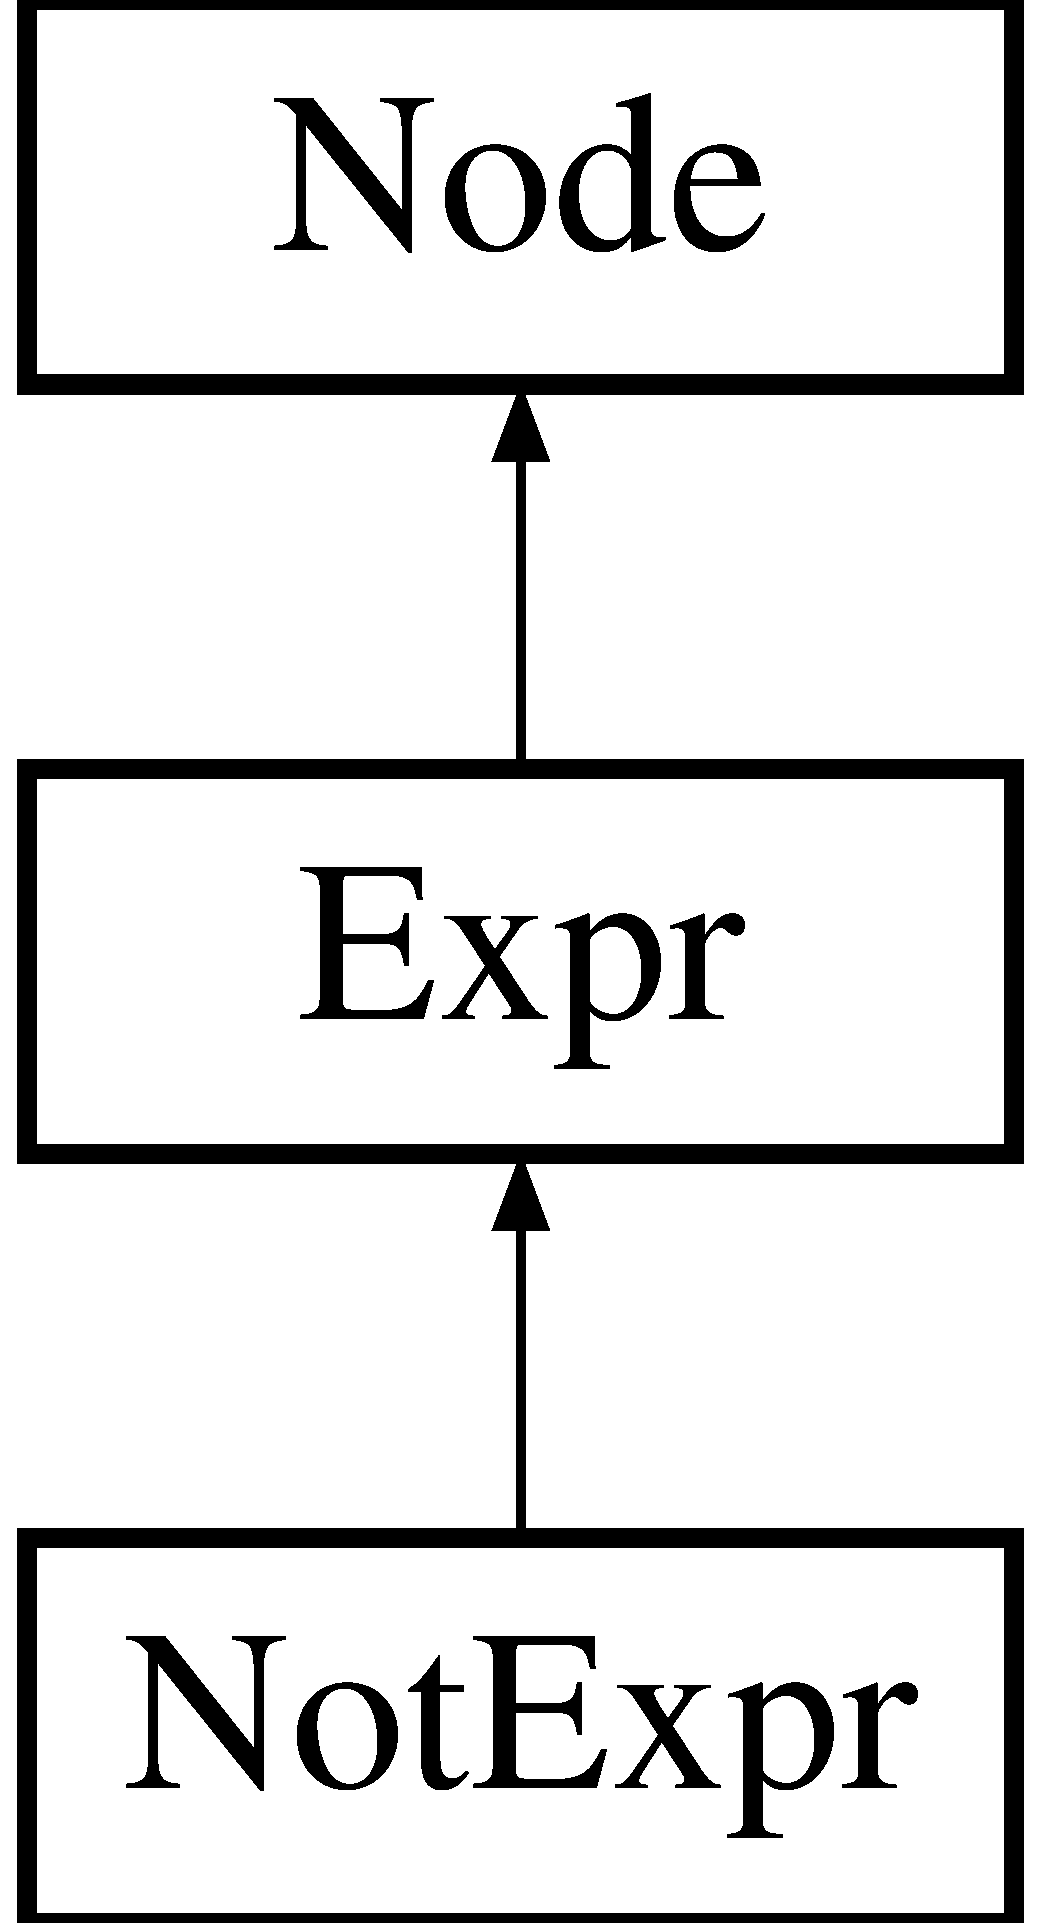
\includegraphics[height=3.000000cm]{classNotExpr}
\end{center}
\end{figure}
\subsection*{Public Member Functions}
\begin{DoxyCompactItemize}
\item 
\hypertarget{classNotExpr_a32d8529fc0f1e411b6a652a372202c7a}{\hyperlink{classNotExpr_a32d8529fc0f1e411b6a652a372202c7a}{Not\-Expr} (\hyperlink{classExpr}{Expr} $\ast$\-\_\-expr)}\label{classNotExpr_a32d8529fc0f1e411b6a652a372202c7a}

\begin{DoxyCompactList}\small\item\em Constructor for \hyperlink{classNotExpr}{Not\-Expr} node. \end{DoxyCompactList}\item 
\hypertarget{classNotExpr_ab49f96d8f23e3fa6bb21376dc0fa5215}{std\-::string \hyperlink{classNotExpr_ab49f96d8f23e3fa6bb21376dc0fa5215}{unparse} ()}\label{classNotExpr_ab49f96d8f23e3fa6bb21376dc0fa5215}

\begin{DoxyCompactList}\small\item\em '!' \hyperlink{classExpr}{Expr} \end{DoxyCompactList}\end{DoxyCompactItemize}


The documentation for this class was generated from the following files\-:\begin{DoxyCompactItemize}
\item 
A\-S\-T.\-h\item 
A\-S\-T.\-cpp\end{DoxyCompactItemize}

\hypertarget{classNotOpToken}{\section{Not\-Op\-Token Class Reference}
\label{classNotOpToken}\index{Not\-Op\-Token@{Not\-Op\-Token}}
}
Inheritance diagram for Not\-Op\-Token\-:\begin{figure}[H]
\begin{center}
\leavevmode
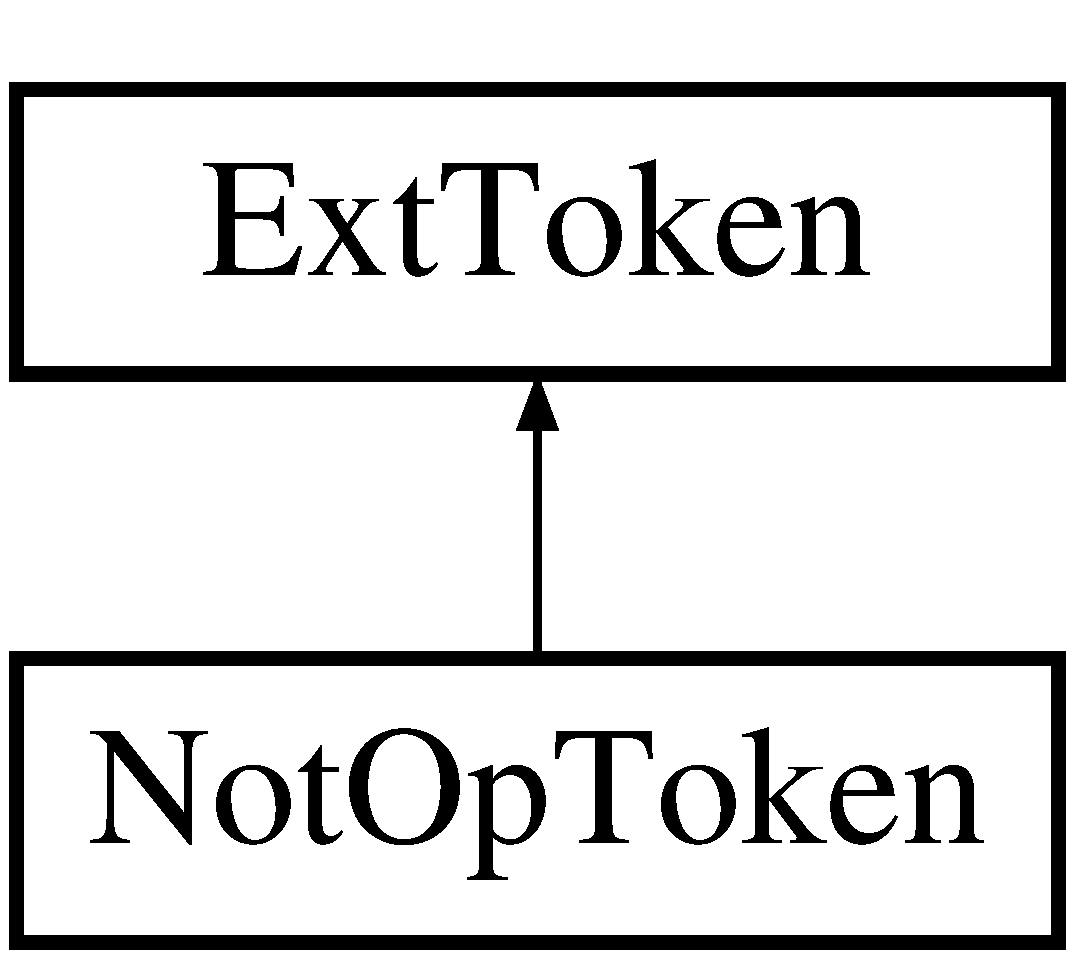
\includegraphics[height=2.000000cm]{classNotOpToken}
\end{center}
\end{figure}
\subsection*{Public Member Functions}
\begin{DoxyCompactItemize}
\item 
\hypertarget{classNotOpToken_afb8b9e96a178b1dfd69abf0a901dfddf}{{\bfseries Not\-Op\-Token} (\hyperlink{classParser}{Parser} $\ast$p, \hyperlink{classToken}{Token} $\ast$t)}\label{classNotOpToken_afb8b9e96a178b1dfd69abf0a901dfddf}

\item 
\hypertarget{classNotOpToken_a55a0dd53742aaca04338c16be079b031}{\hyperlink{classParseResult}{Parse\-Result} {\bfseries nud} ()}\label{classNotOpToken_a55a0dd53742aaca04338c16be079b031}

\item 
\hypertarget{classNotOpToken_a136a11f1e42542a9a58b7c14249c9d23}{std\-::string {\bfseries description} ()}\label{classNotOpToken_a136a11f1e42542a9a58b7c14249c9d23}

\end{DoxyCompactItemize}
\subsection*{Additional Inherited Members}


The documentation for this class was generated from the following file\-:\begin{DoxyCompactItemize}
\item 
ext\-Token.\-h\end{DoxyCompactItemize}

\hypertarget{classParser}{\section{Parser Class Reference}
\label{classParser}\index{Parser@{Parser}}
}
\subsection*{Public Member Functions}
\begin{DoxyCompactItemize}
\item 
\hyperlink{classParser_a12234f6cd36b61af4b50c94a179422c1}{Parser} ()
\item 
\hyperlink{classParser_a3e658b5917a93a3ef648050d060e3a93}{$\sim$\-Parser} ()
\item 
\hypertarget{classParser_a2c1a7aa0b09a43bc1eef460817efb1d6}{\hyperlink{classParseResult}{Parse\-Result} {\bfseries parse} (const char $\ast$text)}\label{classParser_a2c1a7aa0b09a43bc1eef460817efb1d6}

\item 
\hypertarget{classParser_a14e25c84322809e2f060dc530362ea71}{\hyperlink{classParseResult}{Parse\-Result} \hyperlink{classParser_a14e25c84322809e2f060dc530362ea71}{parse\-Program} ()}\label{classParser_a14e25c84322809e2f060dc530362ea71}

\begin{DoxyCompactList}\small\item\em Begins parsing, attaches Root node for A\-S\-T. \end{DoxyCompactList}\item 
\hypertarget{classParser_ac646227983887c1cd13dae67fa1bc142}{\hyperlink{classParseResult}{Parse\-Result} \hyperlink{classParser_ac646227983887c1cd13dae67fa1bc142}{parse\-Decl} ()}\label{classParser_ac646227983887c1cd13dae67fa1bc142}

\begin{DoxyCompactList}\small\item\em Parses declarations. \end{DoxyCompactList}\item 
\hypertarget{classParser_a1e1f83c0f4b11148a356d951f191425e}{\hyperlink{classParseResult}{Parse\-Result} \hyperlink{classParser_a1e1f83c0f4b11148a356d951f191425e}{parse\-Standard\-Decl} ()}\label{classParser_a1e1f83c0f4b11148a356d951f191425e}

\begin{DoxyCompactList}\small\item\em Parses standard\-Decl and make proper A\-S\-T node \hyperlink{classDecl}{Decl} \-:\-:= integer\-Kwd var\-Name $\vert$ float\-Kwd var\-Name $\vert$ string\-Kwd var\-Name. \end{DoxyCompactList}\item 
\hypertarget{classParser_a3a00df25fda2af308b69f05eed14ac69}{\hyperlink{classParseResult}{Parse\-Result} \hyperlink{classParser_a3a00df25fda2af308b69f05eed14ac69}{parse\-Matrix\-Decl} ()}\label{classParser_a3a00df25fda2af308b69f05eed14ac69}

\begin{DoxyCompactList}\small\item\em handles all matrix productions. \end{DoxyCompactList}\item 
\hypertarget{classParser_a452db3def31683cb0305e57a01489bd4}{\hyperlink{classParseResult}{Parse\-Result} \hyperlink{classParser_a452db3def31683cb0305e57a01489bd4}{parse\-Stmts} ()}\label{classParser_a452db3def31683cb0305e57a01489bd4}

\begin{DoxyCompactList}\small\item\em Parses \hyperlink{classStmts}{Stmts}. \end{DoxyCompactList}\item 
\hypertarget{classParser_a9709c4793d0cce012d595f3ee416cd25}{\hyperlink{classParseResult}{Parse\-Result} \hyperlink{classParser_a9709c4793d0cce012d595f3ee416cd25}{parse\-Stmt} ()}\label{classParser_a9709c4793d0cce012d595f3ee416cd25}

\begin{DoxyCompactList}\small\item\em Parses any kind of stmt. \end{DoxyCompactList}\item 
\hypertarget{classParser_a50227dc24dc7a175ac0533d9957dfcf8}{\hyperlink{classParseResult}{Parse\-Result} \hyperlink{classParser_a50227dc24dc7a175ac0533d9957dfcf8}{parse\-Expr} (int rbp)}\label{classParser_a50227dc24dc7a175ac0533d9957dfcf8}

\begin{DoxyCompactList}\small\item\em calls different parse functions for expression \end{DoxyCompactList}\item 
\hypertarget{classParser_ad40f1e5e4c66814f959d982f94b767a3}{\hyperlink{classParseResult}{Parse\-Result} {\bfseries parse\-True\-Kwd} ()}\label{classParser_ad40f1e5e4c66814f959d982f94b767a3}

\item 
\hypertarget{classParser_a56f03d2e70d12648c55ce56a11e63324}{\hyperlink{classParseResult}{Parse\-Result} {\bfseries parse\-False\-Kwd} ()}\label{classParser_a56f03d2e70d12648c55ce56a11e63324}

\item 
\hypertarget{classParser_a2b200b744e5bedf82ef6f610d7877cfc}{\hyperlink{classParseResult}{Parse\-Result} {\bfseries parse\-Int\-Const} ()}\label{classParser_a2b200b744e5bedf82ef6f610d7877cfc}

\item 
\hypertarget{classParser_aaf7b1176fd53246f59577c7eec8b9d22}{\hyperlink{classParseResult}{Parse\-Result} {\bfseries parse\-Float\-Const} ()}\label{classParser_aaf7b1176fd53246f59577c7eec8b9d22}

\item 
\hypertarget{classParser_a4d8930d45c2b730912154c46cc54833c}{\hyperlink{classParseResult}{Parse\-Result} {\bfseries parse\-String\-Const} ()}\label{classParser_a4d8930d45c2b730912154c46cc54833c}

\item 
\hypertarget{classParser_a49c9b3d31ca060c97873e5485d518da3}{\hyperlink{classParseResult}{Parse\-Result} {\bfseries parse\-Char\-Const} ()}\label{classParser_a49c9b3d31ca060c97873e5485d518da3}

\item 
\hypertarget{classParser_a8c1baf62f71da64590e883e51ce622ca}{\hyperlink{classParseResult}{Parse\-Result} {\bfseries parse\-Variable\-Name} ()}\label{classParser_a8c1baf62f71da64590e883e51ce622ca}

\item 
\hypertarget{classParser_aec4c38e1e63c9becfd3a8fc4a1a73f01}{\hyperlink{classParseResult}{Parse\-Result} {\bfseries parse\-Nested\-Expr} ()}\label{classParser_aec4c38e1e63c9becfd3a8fc4a1a73f01}

\item 
\hypertarget{classParser_a1503ceff46112d6d4f0e01b5fb77afcd}{\hyperlink{classParseResult}{Parse\-Result} {\bfseries parse\-Not\-Expr} ()}\label{classParser_a1503ceff46112d6d4f0e01b5fb77afcd}

\item 
\hypertarget{classParser_aa24c33b04779801b330d7fe5a74349e5}{\hyperlink{classParseResult}{Parse\-Result} {\bfseries parse\-Let\-Expr} ()}\label{classParser_aa24c33b04779801b330d7fe5a74349e5}

\item 
\hypertarget{classParser_a555bc6f671d408208e6d049f8e9f3c86}{\hyperlink{classParseResult}{Parse\-Result} {\bfseries parse\-If\-Expr} ()}\label{classParser_a555bc6f671d408208e6d049f8e9f3c86}

\item 
\hypertarget{classParser_ae09cb2b5a7f80c6ad4ad9ccf27a746ca}{\hyperlink{classParseResult}{Parse\-Result} {\bfseries parse\-Addition} (\hyperlink{classParseResult}{Parse\-Result} left)}\label{classParser_ae09cb2b5a7f80c6ad4ad9ccf27a746ca}

\item 
\hypertarget{classParser_a52e6a57d53fc98e5819cc51b3cbe5bd5}{\hyperlink{classParseResult}{Parse\-Result} {\bfseries parse\-Multiplication} (\hyperlink{classParseResult}{Parse\-Result} left)}\label{classParser_a52e6a57d53fc98e5819cc51b3cbe5bd5}

\item 
\hypertarget{classParser_ac22cf1f77e0ca4c23942d5cbcc47eb37}{\hyperlink{classParseResult}{Parse\-Result} {\bfseries parse\-Subtraction} (\hyperlink{classParseResult}{Parse\-Result} left)}\label{classParser_ac22cf1f77e0ca4c23942d5cbcc47eb37}

\item 
\hypertarget{classParser_ad05e6cd1bf83179ecb727b83cbbd0c4e}{\hyperlink{classParseResult}{Parse\-Result} {\bfseries parse\-Division} (\hyperlink{classParseResult}{Parse\-Result} left)}\label{classParser_ad05e6cd1bf83179ecb727b83cbbd0c4e}

\item 
\hypertarget{classParser_ab42ecabc4dbe601d5ed9667351c0c0b8}{\hyperlink{classParseResult}{Parse\-Result} {\bfseries parse\-Relational\-Expr} (\hyperlink{classParseResult}{Parse\-Result} left)}\label{classParser_ab42ecabc4dbe601d5ed9667351c0c0b8}

\item 
\hypertarget{classParser_a3199aab5275c8b6477245eb866fabf35}{void {\bfseries match} (token\-Type tt)}\label{classParser_a3199aab5275c8b6477245eb866fabf35}

\item 
\hypertarget{classParser_a151ffb920a67527813d77bc4ba44c4a7}{bool {\bfseries attempt\-Match} (token\-Type tt)}\label{classParser_a151ffb920a67527813d77bc4ba44c4a7}

\item 
\hypertarget{classParser_a67a10b685bd263477b5f59f1923cdec3}{bool {\bfseries next\-Is} (token\-Type tt)}\label{classParser_a67a10b685bd263477b5f59f1923cdec3}

\item 
\hypertarget{classParser_a324a5bb61c9dfc645300a92aecd6fe69}{void {\bfseries next\-Token} ()}\label{classParser_a324a5bb61c9dfc645300a92aecd6fe69}

\item 
\hypertarget{classParser_a1f45059a13bc0c98355278a9ca9feed9}{std\-::string {\bfseries terminal\-Description} (token\-Type terminal)}\label{classParser_a1f45059a13bc0c98355278a9ca9feed9}

\item 
\hypertarget{classParser_a341bee73e8b1e8558505a237846b16b3}{std\-::string {\bfseries make\-Error\-Msg} (token\-Type terminal)}\label{classParser_a341bee73e8b1e8558505a237846b16b3}

\item 
\hypertarget{classParser_ad38e58ddee85db2aecbd3c7bdcf42116}{std\-::string {\bfseries make\-Error\-Msg\-Expected} (token\-Type terminal)}\label{classParser_ad38e58ddee85db2aecbd3c7bdcf42116}

\item 
\hypertarget{classParser_a60c23daeffb7ced92599e4f2555f71c9}{std\-::string {\bfseries make\-Error\-Msg} (const char $\ast$msg)}\label{classParser_a60c23daeffb7ced92599e4f2555f71c9}

\end{DoxyCompactItemize}
\subsection*{Public Attributes}
\begin{DoxyCompactItemize}
\item 
\hypertarget{classParser_a3606ff327be18af7f76df95f50851633}{\hyperlink{classExtToken}{Ext\-Token} $\ast$ {\bfseries tokens}}\label{classParser_a3606ff327be18af7f76df95f50851633}

\item 
\hypertarget{classParser_a75ab2e2b9385c14e5f967f873340ed11}{\hyperlink{classExtToken}{Ext\-Token} $\ast$ {\bfseries curr\-Token}}\label{classParser_a75ab2e2b9385c14e5f967f873340ed11}

\item 
\hypertarget{classParser_a4bcf7560a5ea1b486bbe4bb54a5a22eb}{\hyperlink{classExtToken}{Ext\-Token} $\ast$ {\bfseries prev\-Token}}\label{classParser_a4bcf7560a5ea1b486bbe4bb54a5a22eb}

\item 
\hypertarget{classParser_a0910de176dcc1cdfbf7ad99622ce9dd5}{\hyperlink{classToken}{Token} $\ast$ {\bfseries stokens}}\label{classParser_a0910de176dcc1cdfbf7ad99622ce9dd5}

\item 
\hypertarget{classParser_ab2ef99ea9e732f5fd176b3949a6c32af}{\hyperlink{classScanner}{Scanner} $\ast$ {\bfseries s}}\label{classParser_ab2ef99ea9e732f5fd176b3949a6c32af}

\end{DoxyCompactItemize}


\subsection{Constructor \& Destructor Documentation}
\hypertarget{classParser_a12234f6cd36b61af4b50c94a179422c1}{\index{Parser@{Parser}!Parser@{Parser}}
\index{Parser@{Parser}!Parser@{Parser}}
\subsubsection[{Parser}]{\setlength{\rightskip}{0pt plus 5cm}Parser\-::\-Parser (
\begin{DoxyParamCaption}
{}
\end{DoxyParamCaption}
)}}\label{classParser_a12234f6cd36b61af4b50c94a179422c1}
Constructor for parser \hypertarget{classParser_a3e658b5917a93a3ef648050d060e3a93}{\index{Parser@{Parser}!$\sim$\-Parser@{$\sim$\-Parser}}
\index{$\sim$\-Parser@{$\sim$\-Parser}!Parser@{Parser}}
\subsubsection[{$\sim$\-Parser}]{\setlength{\rightskip}{0pt plus 5cm}Parser\-::$\sim$\-Parser (
\begin{DoxyParamCaption}
{}
\end{DoxyParamCaption}
)}}\label{classParser_a3e658b5917a93a3ef648050d060e3a93}
Destructor for parser. 

The documentation for this class was generated from the following files\-:\begin{DoxyCompactItemize}
\item 
parser.\-h\item 
parser.\-cpp\end{DoxyCompactItemize}

\hypertarget{classParseResult}{\section{Parse\-Result Class Reference}
\label{classParseResult}\index{Parse\-Result@{Parse\-Result}}
}
\subsection*{Public Attributes}
\begin{DoxyCompactItemize}
\item 
\hypertarget{classParseResult_ab2dd8deb95c5177148f488ca5d31307a}{std\-::string {\bfseries errors}}\label{classParseResult_ab2dd8deb95c5177148f488ca5d31307a}

\item 
\hypertarget{classParseResult_aa04c6ed3cba109f276e5bc089ca2ff15}{\hyperlink{classNode}{Node} $\ast$ {\bfseries ast}}\label{classParseResult_aa04c6ed3cba109f276e5bc089ca2ff15}

\item 
\hypertarget{classParseResult_a64eb6658c1fc5bbf35fdce181f6845d5}{bool {\bfseries ok}}\label{classParseResult_a64eb6658c1fc5bbf35fdce181f6845d5}

\end{DoxyCompactItemize}


The documentation for this class was generated from the following files\-:\begin{DoxyCompactItemize}
\item 
parse\-Result.\-h\item 
parse\-Result.\-cpp\end{DoxyCompactItemize}

\hypertarget{classParserTestSuite}{\section{Parser\-Test\-Suite Class Reference}
\label{classParserTestSuite}\index{Parser\-Test\-Suite@{Parser\-Test\-Suite}}
}
Inheritance diagram for Parser\-Test\-Suite\-:\begin{figure}[H]
\begin{center}
\leavevmode
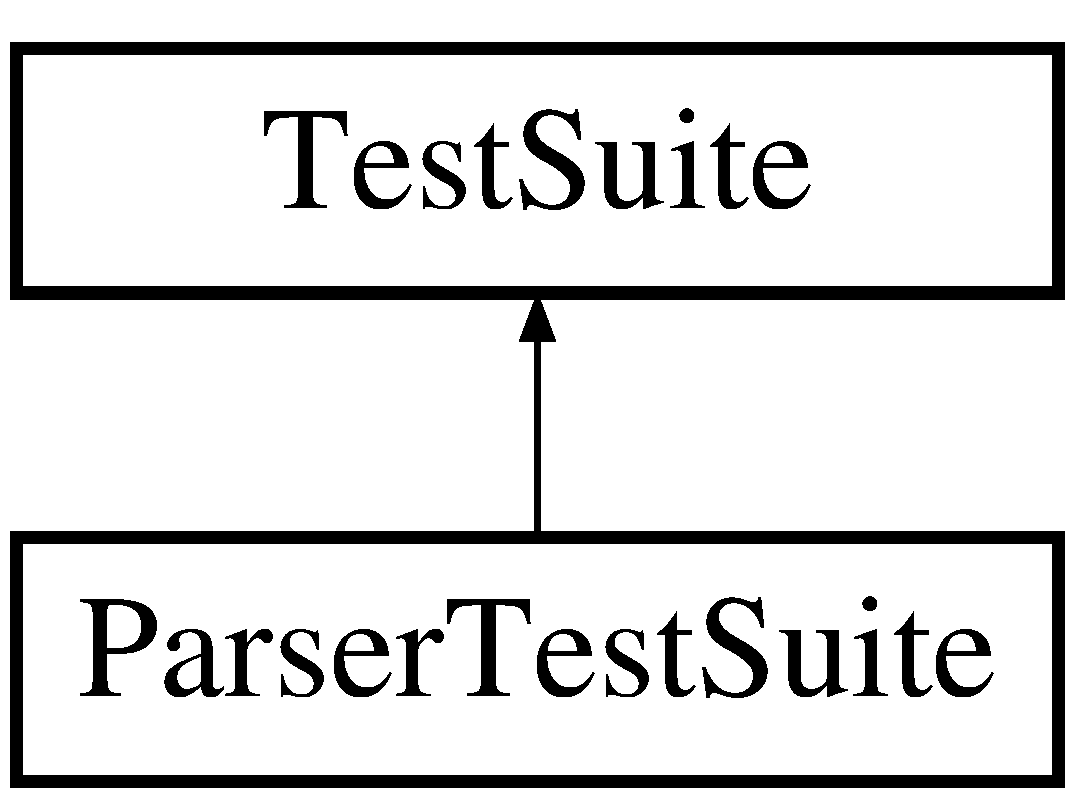
\includegraphics[height=2.000000cm]{classParserTestSuite}
\end{center}
\end{figure}
\subsection*{Public Member Functions}
\begin{DoxyCompactItemize}
\item 
\hypertarget{classParserTestSuite_ab7eff3217b5e28c9003f27c51da107ac}{void {\bfseries test\-\_\-setup\-\_\-code} ()}\label{classParserTestSuite_ab7eff3217b5e28c9003f27c51da107ac}

\item 
\hypertarget{classParserTestSuite_ac4a829a66a1582bee38e90ac3f0355f4}{void {\bfseries test\-\_\-parse\-\_\-bad\-\_\-syntax} ()}\label{classParserTestSuite_ac4a829a66a1582bee38e90ac3f0355f4}

\item 
\hypertarget{classParserTestSuite_a26eed485bc2671f4ac256ef97a21b704}{void {\bfseries test\-\_\-parse\-\_\-sample\-\_\-1} ()}\label{classParserTestSuite_a26eed485bc2671f4ac256ef97a21b704}

\item 
\hypertarget{classParserTestSuite_a0f1d6af1e07e35541fb83416d5e3e229}{void {\bfseries test\-\_\-parse\-\_\-sample\-\_\-2} ()}\label{classParserTestSuite_a0f1d6af1e07e35541fb83416d5e3e229}

\item 
\hypertarget{classParserTestSuite_aecc132f6b6dbb2e5bba08baec64f3f65}{void {\bfseries test\-\_\-parse\-\_\-sample\-\_\-3} ()}\label{classParserTestSuite_aecc132f6b6dbb2e5bba08baec64f3f65}

\item 
\hypertarget{classParserTestSuite_a6e5dfaf7b8ddc98001a4fec39b3f0a79}{void {\bfseries test\-\_\-parse\-\_\-sample\-\_\-4} ()}\label{classParserTestSuite_a6e5dfaf7b8ddc98001a4fec39b3f0a79}

\item 
\hypertarget{classParserTestSuite_a5b9a3cf2b76271244baaaaa4c8b7f7d5}{void {\bfseries test\-\_\-parse\-\_\-sample\-\_\-5} ()}\label{classParserTestSuite_a5b9a3cf2b76271244baaaaa4c8b7f7d5}

\item 
\hypertarget{classParserTestSuite_ae59d0f6d92f8d83833d51ef01479fdeb}{void {\bfseries test\-\_\-parse\-\_\-mysample} ()}\label{classParserTestSuite_ae59d0f6d92f8d83833d51ef01479fdeb}

\item 
\hypertarget{classParserTestSuite_a379db1a22b2c32defb8395b9b2166f76}{void {\bfseries test\-\_\-parse\-\_\-forest\-Loss\-V2} ()}\label{classParserTestSuite_a379db1a22b2c32defb8395b9b2166f76}

\end{DoxyCompactItemize}
\subsection*{Public Attributes}
\begin{DoxyCompactItemize}
\item 
\hypertarget{classParserTestSuite_a0c4943b3d23b79be363ba9e1ac7c02ed}{\hyperlink{classScanner}{Scanner} $\ast$ {\bfseries s}}\label{classParserTestSuite_a0c4943b3d23b79be363ba9e1ac7c02ed}

\item 
\hypertarget{classParserTestSuite_a1d637f2f8be1326423ee5b4fd270c553}{\hyperlink{classParser}{Parser} $\ast$ {\bfseries p}}\label{classParserTestSuite_a1d637f2f8be1326423ee5b4fd270c553}

\end{DoxyCompactItemize}


The documentation for this class was generated from the following file\-:\begin{DoxyCompactItemize}
\item 
parser\-\_\-tests.\-h\end{DoxyCompactItemize}

\hypertarget{classPlusSignToken}{\section{Plus\-Sign\-Token Class Reference}
\label{classPlusSignToken}\index{Plus\-Sign\-Token@{Plus\-Sign\-Token}}
}
Inheritance diagram for Plus\-Sign\-Token\-:\begin{figure}[H]
\begin{center}
\leavevmode
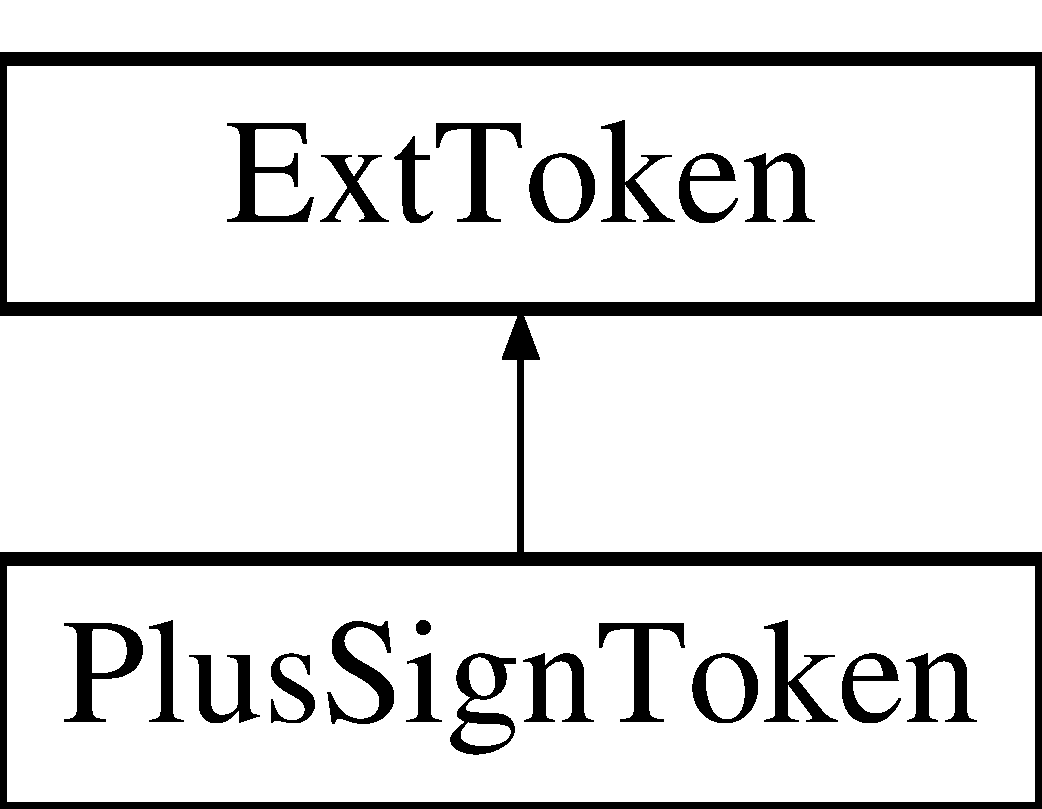
\includegraphics[height=2.000000cm]{classPlusSignToken}
\end{center}
\end{figure}
\subsection*{Public Member Functions}
\begin{DoxyCompactItemize}
\item 
\hypertarget{classPlusSignToken_ad480457c426f911f8286a73e8cf7f949}{{\bfseries Plus\-Sign\-Token} (\hyperlink{classParser}{Parser} $\ast$p, \hyperlink{classToken}{Token} $\ast$t)}\label{classPlusSignToken_ad480457c426f911f8286a73e8cf7f949}

\item 
\hypertarget{classPlusSignToken_a4d79a17891f92800259308ce71402526}{\hyperlink{classParseResult}{Parse\-Result} {\bfseries led} (\hyperlink{classParseResult}{Parse\-Result} left)}\label{classPlusSignToken_a4d79a17891f92800259308ce71402526}

\item 
\hypertarget{classPlusSignToken_a61a05ac9660848e13da97d5746808868}{std\-::string {\bfseries description} ()}\label{classPlusSignToken_a61a05ac9660848e13da97d5746808868}

\item 
\hypertarget{classPlusSignToken_a80753eec970928e042da350df83150f2}{int {\bfseries lbp} ()}\label{classPlusSignToken_a80753eec970928e042da350df83150f2}

\end{DoxyCompactItemize}
\subsection*{Additional Inherited Members}


The documentation for this class was generated from the following file\-:\begin{DoxyCompactItemize}
\item 
ext\-Token.\-h\end{DoxyCompactItemize}

\hypertarget{classPrintStmt}{\section{Print\-Stmt Class Reference}
\label{classPrintStmt}\index{Print\-Stmt@{Print\-Stmt}}
}
Inheritance diagram for Print\-Stmt\-:\begin{figure}[H]
\begin{center}
\leavevmode
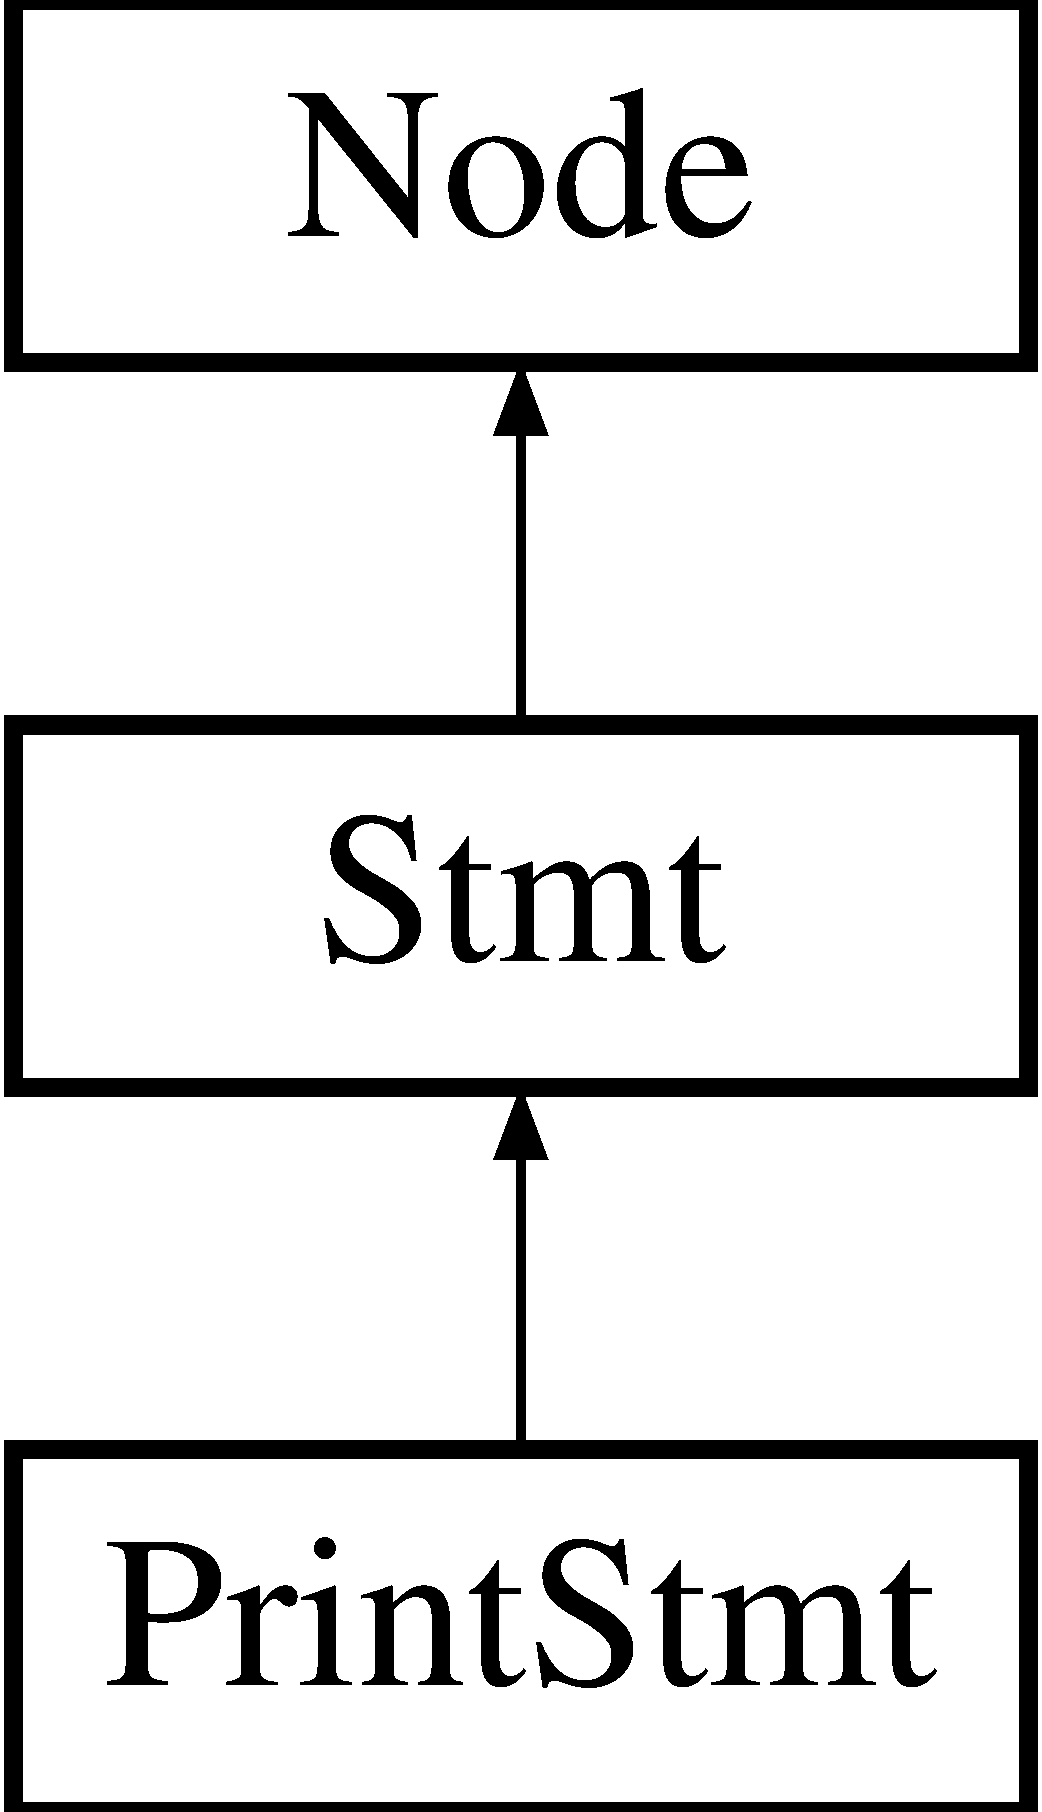
\includegraphics[height=3.000000cm]{classPrintStmt}
\end{center}
\end{figure}
\subsection*{Public Member Functions}
\begin{DoxyCompactItemize}
\item 
\hypertarget{classPrintStmt_a02701fedccfe3e4f509e628286e0ecf1}{\hyperlink{classPrintStmt_a02701fedccfe3e4f509e628286e0ecf1}{Print\-Stmt} (\hyperlink{classExpr}{Expr} $\ast$\-\_\-expr)}\label{classPrintStmt_a02701fedccfe3e4f509e628286e0ecf1}

\begin{DoxyCompactList}\small\item\em Constructor for \hyperlink{classPrintStmt}{Print\-Stmt} node. \end{DoxyCompactList}\item 
\hypertarget{classPrintStmt_aa3c9ad246b75bd45a48e563500b5109f}{std\-::string \hyperlink{classPrintStmt_aa3c9ad246b75bd45a48e563500b5109f}{unparse} ()}\label{classPrintStmt_aa3c9ad246b75bd45a48e563500b5109f}

\begin{DoxyCompactList}\small\item\em 'print' '(' \hyperlink{classExpr}{Expr} ')' ';' \end{DoxyCompactList}\end{DoxyCompactItemize}


The documentation for this class was generated from the following files\-:\begin{DoxyCompactItemize}
\item 
A\-S\-T.\-h\item 
A\-S\-T.\-cpp\end{DoxyCompactItemize}

\hypertarget{classProgram}{\section{Program Class Reference}
\label{classProgram}\index{Program@{Program}}
}
Inheritance diagram for Program\-:\begin{figure}[H]
\begin{center}
\leavevmode
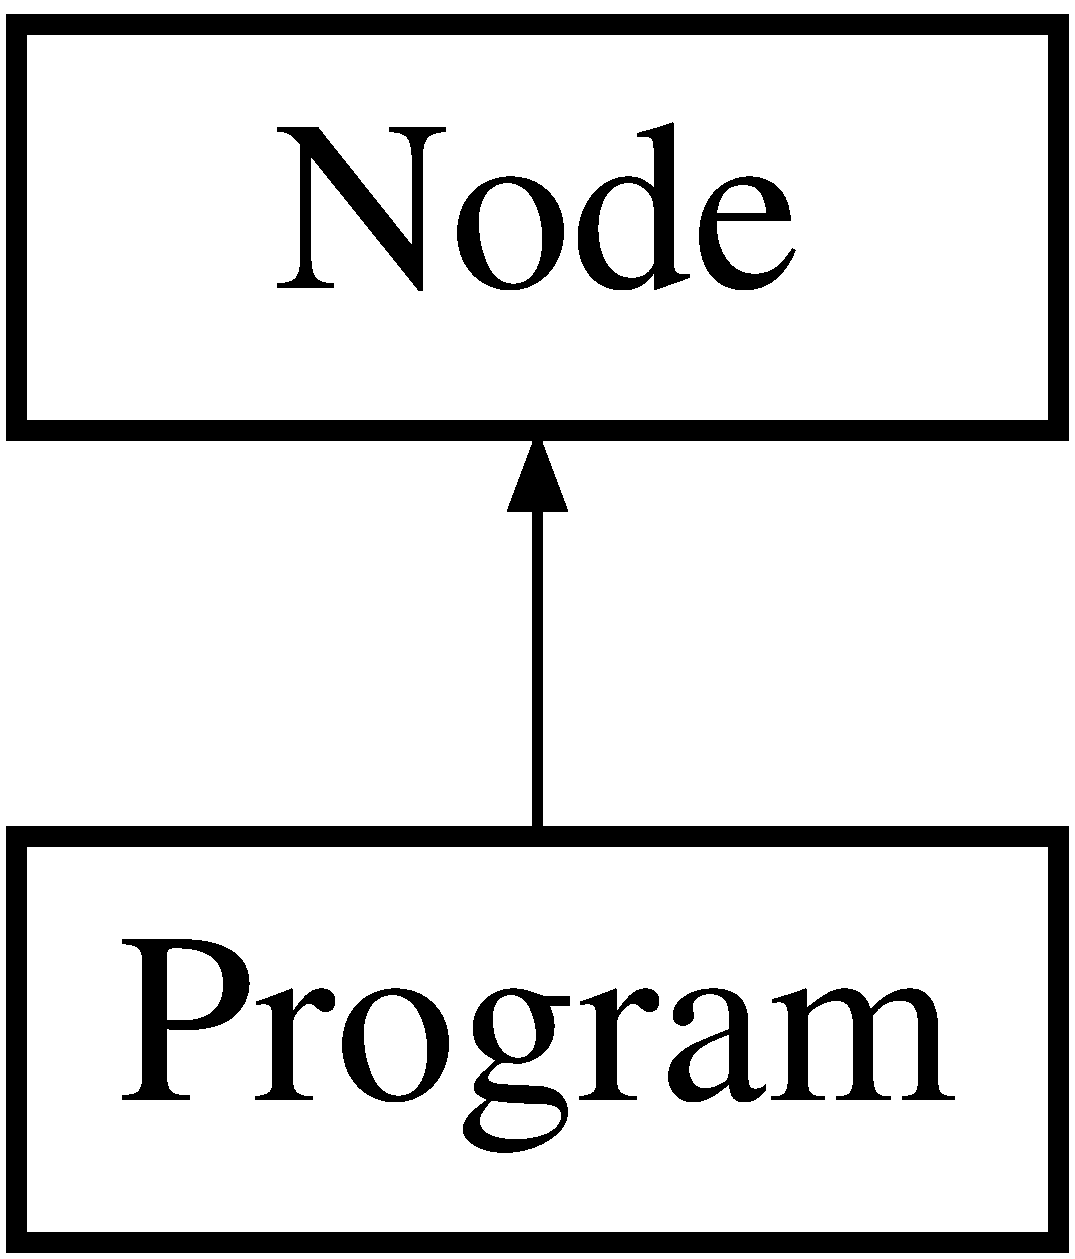
\includegraphics[height=2.000000cm]{classProgram}
\end{center}
\end{figure}
\subsection*{Public Member Functions}
\begin{DoxyCompactItemize}
\item 
\hypertarget{classProgram_a0fe9e8c0aab485a521a899c9e651e8b5}{\hyperlink{classProgram_a0fe9e8c0aab485a521a899c9e651e8b5}{Program} (std\-::string \-\_\-varname, \hyperlink{classStmts}{Stmts} $\ast$\-\_\-stmts)}\label{classProgram_a0fe9e8c0aab485a521a899c9e651e8b5}

\begin{DoxyCompactList}\small\item\em Constructor for Root/\-Program node. \end{DoxyCompactList}\item 
\hypertarget{classProgram_a33c78e36a63c63e5821b7747bec7b644}{std\-::string \hyperlink{classProgram_a33c78e36a63c63e5821b7747bec7b644}{unparse} ()}\label{classProgram_a33c78e36a63c63e5821b7747bec7b644}

\begin{DoxyCompactList}\small\item\em var\-Name '(' ')' '\{' \hyperlink{classStmts}{Stmts} '\}' \end{DoxyCompactList}\end{DoxyCompactItemize}


The documentation for this class was generated from the following files\-:\begin{DoxyCompactItemize}
\item 
A\-S\-T.\-h\item 
A\-S\-T.\-cpp\end{DoxyCompactItemize}

\hypertarget{classRegexTestSuite}{\section{Regex\-Test\-Suite Class Reference}
\label{classRegexTestSuite}\index{Regex\-Test\-Suite@{Regex\-Test\-Suite}}
}
Inheritance diagram for Regex\-Test\-Suite\-:\begin{figure}[H]
\begin{center}
\leavevmode
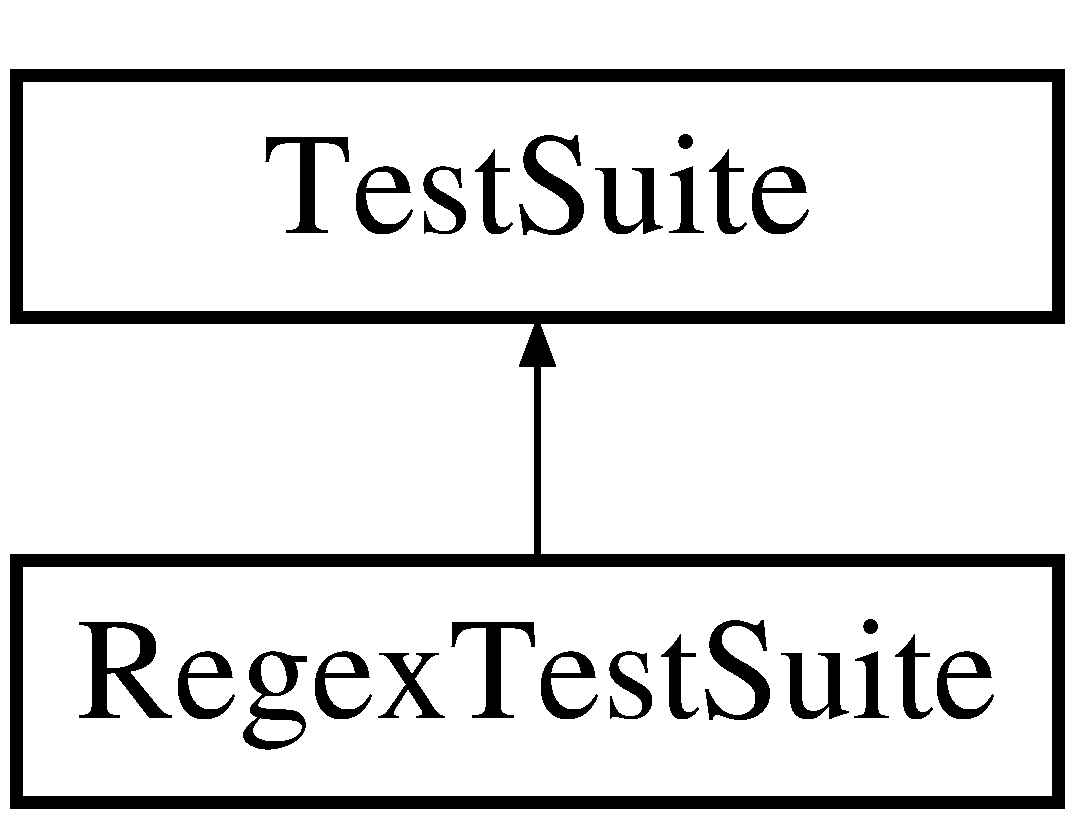
\includegraphics[height=2.000000cm]{classRegexTestSuite}
\end{center}
\end{figure}
\subsection*{Public Member Functions}
\begin{DoxyCompactItemize}
\item 
\hypertarget{classRegexTestSuite_aac0838d917fd9fd6cc71ee086c644555}{void {\bfseries test\-\_\-make\-\_\-match\-Regex\-\_\-match} (void)}\label{classRegexTestSuite_aac0838d917fd9fd6cc71ee086c644555}

\item 
\hypertarget{classRegexTestSuite_ad9c02b9f4fd7feca750d476cda8e0c60}{void {\bfseries test\-\_\-make\-\_\-match\-Regex\-\_\-no\-\_\-match} (void)}\label{classRegexTestSuite_ad9c02b9f4fd7feca750d476cda8e0c60}

\item 
\hypertarget{classRegexTestSuite_a0f46b90e2c0a1c98750a3335d086979a}{void {\bfseries test\-\_\-make\-\_\-match\-Regex\-\_\-match\-\_\-string\-\_\-copy} (void)}\label{classRegexTestSuite_a0f46b90e2c0a1c98750a3335d086979a}

\end{DoxyCompactItemize}


The documentation for this class was generated from the following file\-:\begin{DoxyCompactItemize}
\item 
regex\-\_\-tests.\-h\end{DoxyCompactItemize}

\hypertarget{classRelationalOpToken}{\section{Relational\-Op\-Token Class Reference}
\label{classRelationalOpToken}\index{Relational\-Op\-Token@{Relational\-Op\-Token}}
}
Inheritance diagram for Relational\-Op\-Token\-:\begin{figure}[H]
\begin{center}
\leavevmode
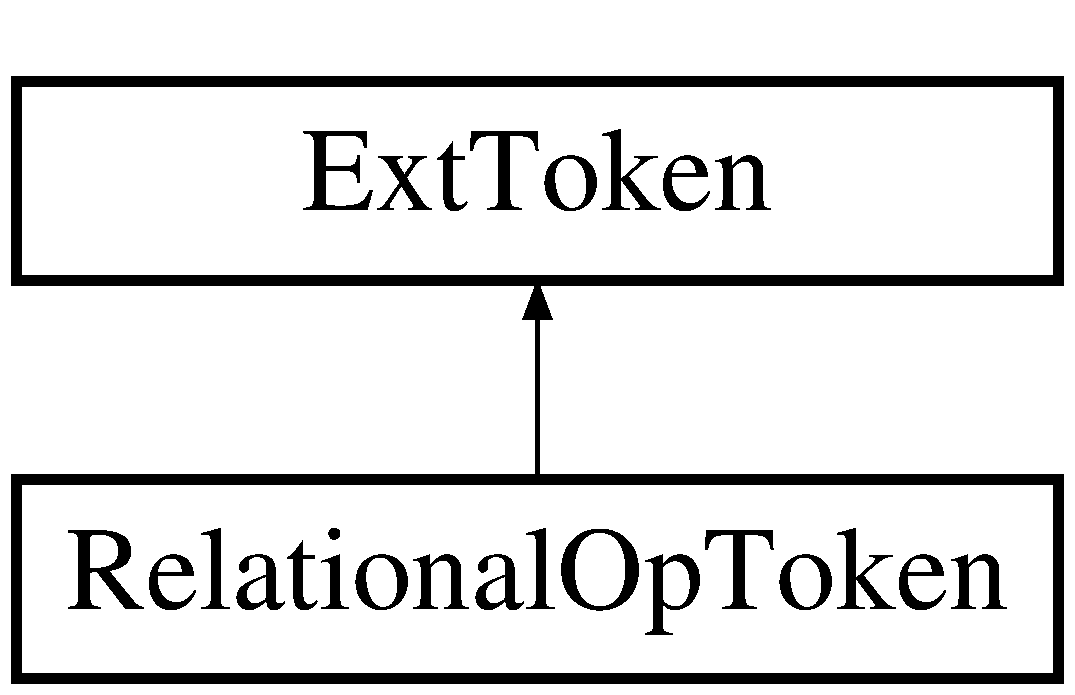
\includegraphics[height=2.000000cm]{classRelationalOpToken}
\end{center}
\end{figure}
\subsection*{Public Member Functions}
\begin{DoxyCompactItemize}
\item 
\hypertarget{classRelationalOpToken_a1ede45cf178138ff12beba209681be51}{{\bfseries Relational\-Op\-Token} (\hyperlink{classParser}{Parser} $\ast$p, \hyperlink{classToken}{Token} $\ast$t, std\-::string d)}\label{classRelationalOpToken_a1ede45cf178138ff12beba209681be51}

\item 
\hypertarget{classRelationalOpToken_a426c64391e7b3272d8e6277964730e05}{\hyperlink{classParseResult}{Parse\-Result} {\bfseries led} (\hyperlink{classParseResult}{Parse\-Result} left)}\label{classRelationalOpToken_a426c64391e7b3272d8e6277964730e05}

\item 
\hypertarget{classRelationalOpToken_ada096491d9553aea21089230489d6aef}{int {\bfseries lbp} ()}\label{classRelationalOpToken_ada096491d9553aea21089230489d6aef}

\end{DoxyCompactItemize}
\subsection*{Additional Inherited Members}


The documentation for this class was generated from the following file\-:\begin{DoxyCompactItemize}
\item 
ext\-Token.\-h\end{DoxyCompactItemize}

\hypertarget{classRepeatStmt}{\section{Repeat\-Stmt Class Reference}
\label{classRepeatStmt}\index{Repeat\-Stmt@{Repeat\-Stmt}}
}
Inheritance diagram for Repeat\-Stmt\-:\begin{figure}[H]
\begin{center}
\leavevmode
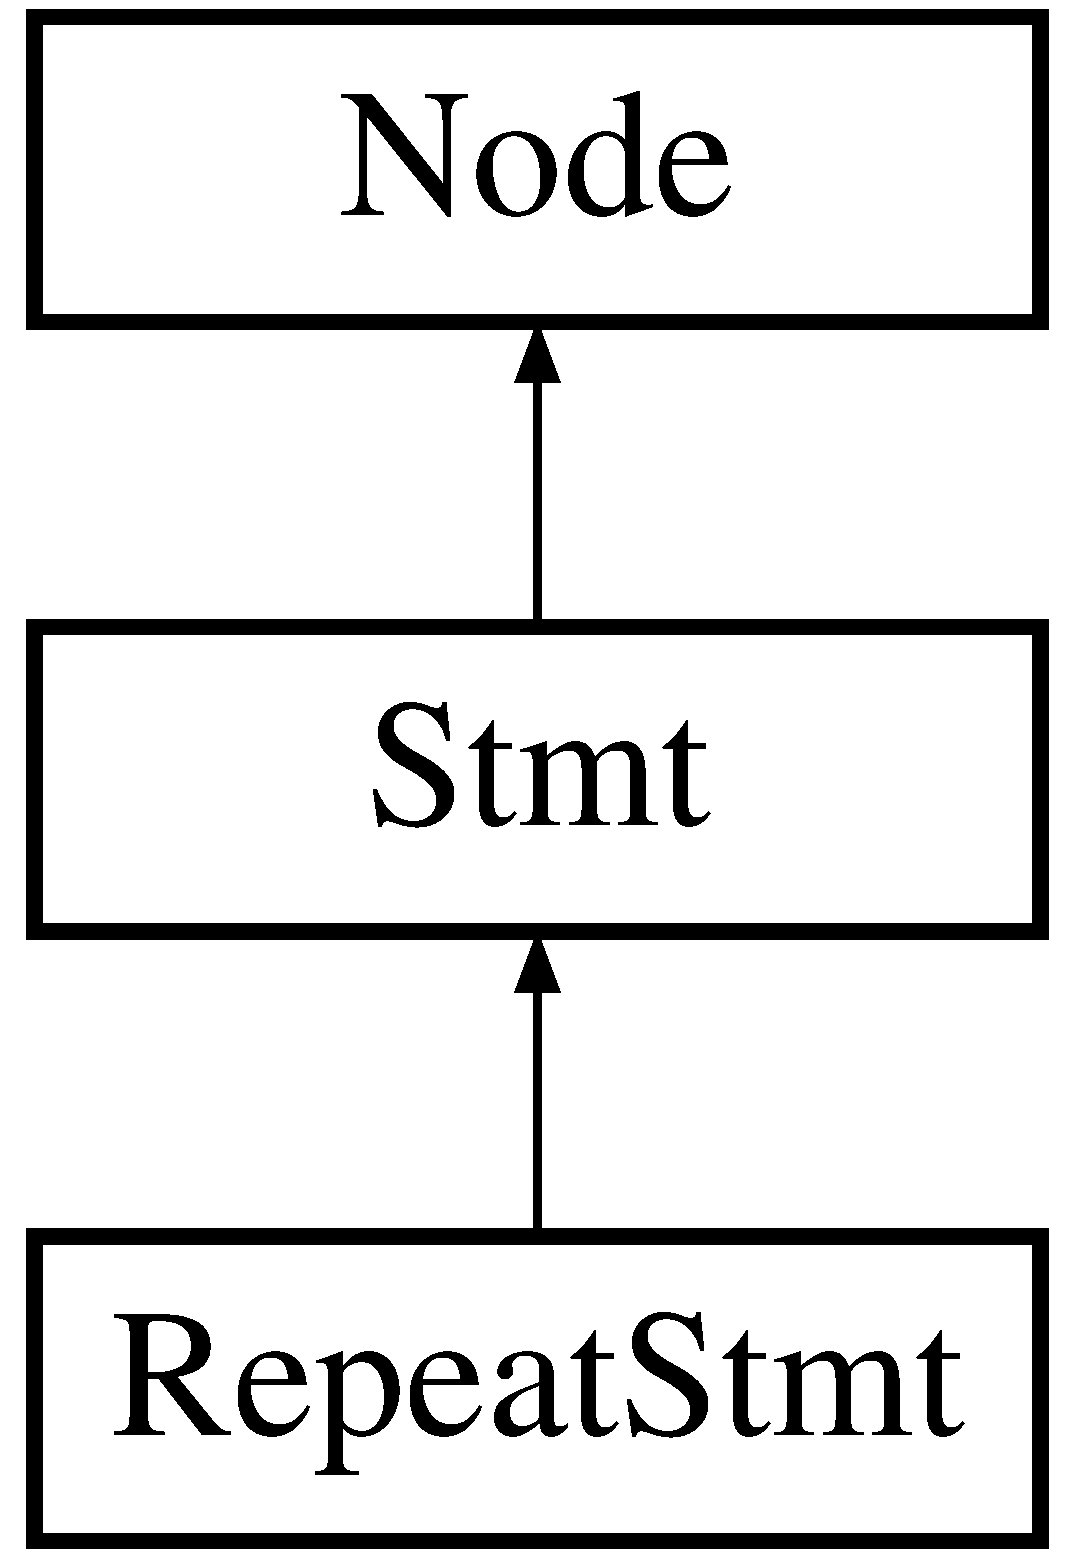
\includegraphics[height=3.000000cm]{classRepeatStmt}
\end{center}
\end{figure}
\subsection*{Public Member Functions}
\begin{DoxyCompactItemize}
\item 
\hypertarget{classRepeatStmt_a080f13ebf0369f2babc0d14e3c3f2bcf}{\hyperlink{classRepeatStmt_a080f13ebf0369f2babc0d14e3c3f2bcf}{Repeat\-Stmt} (std\-::string \-\_\-varname, \hyperlink{classExpr}{Expr} $\ast$\-\_\-expr1, \hyperlink{classExpr}{Expr} $\ast$\-\_\-expr2, \hyperlink{classStmt}{Stmt} $\ast$\-\_\-stmt)}\label{classRepeatStmt_a080f13ebf0369f2babc0d14e3c3f2bcf}

\begin{DoxyCompactList}\small\item\em Constructor for \hyperlink{classRepeatStmt}{Repeat\-Stmt} node. \end{DoxyCompactList}\item 
\hypertarget{classRepeatStmt_a9ccc876694fd9b60671818bb9c81447e}{std\-::string \hyperlink{classRepeatStmt_a9ccc876694fd9b60671818bb9c81447e}{unparse} ()}\label{classRepeatStmt_a9ccc876694fd9b60671818bb9c81447e}

\begin{DoxyCompactList}\small\item\em 'for' '(' var\-Name '=' \hyperlink{classExpr}{Expr} '\-:' \hyperlink{classExpr}{Expr} ')' \hyperlink{classStmt}{Stmt} \end{DoxyCompactList}\end{DoxyCompactItemize}


The documentation for this class was generated from the following files\-:\begin{DoxyCompactItemize}
\item 
A\-S\-T.\-h\item 
A\-S\-T.\-cpp\end{DoxyCompactItemize}

\hypertarget{classScanner}{\section{Scanner Class Reference}
\label{classScanner}\index{Scanner@{Scanner}}
}
\subsection*{Public Member Functions}
\begin{DoxyCompactItemize}
\item 
\hypertarget{classScanner_a40f021dac0075b146272e42d425b2ba5}{\hyperlink{classToken}{Token} $\ast$ {\bfseries scan} (const char $\ast$text)}\label{classScanner_a40f021dac0075b146272e42d425b2ba5}

\end{DoxyCompactItemize}


The documentation for this class was generated from the following files\-:\begin{DoxyCompactItemize}
\item 
scanner.\-h\item 
scanner.\-cpp\end{DoxyCompactItemize}

\hypertarget{classScannerTestSuite}{\section{Scanner\-Test\-Suite Class Reference}
\label{classScannerTestSuite}\index{Scanner\-Test\-Suite@{Scanner\-Test\-Suite}}
}
Inheritance diagram for Scanner\-Test\-Suite\-:\begin{figure}[H]
\begin{center}
\leavevmode
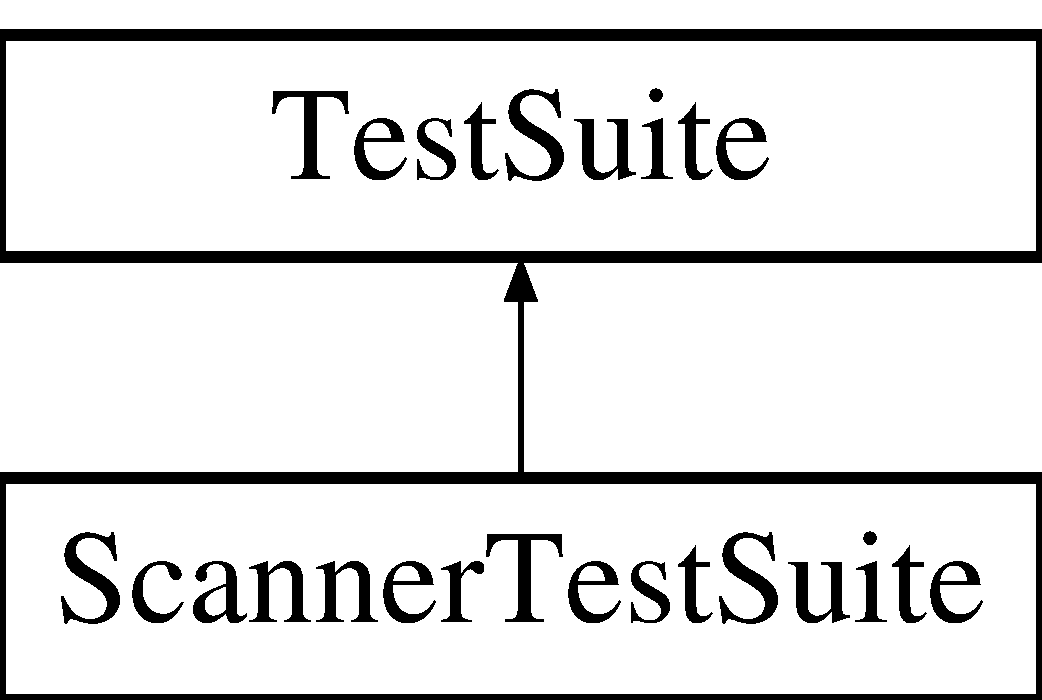
\includegraphics[height=2.000000cm]{classScannerTestSuite}
\end{center}
\end{figure}
\subsection*{Public Member Functions}
\begin{DoxyCompactItemize}
\item 
\hypertarget{classScannerTestSuite_ade832b9b4b3bd92980d43c4050cebd2c}{void {\bfseries test\-\_\-setup\-\_\-code} ()}\label{classScannerTestSuite_ade832b9b4b3bd92980d43c4050cebd2c}

\item 
\hypertarget{classScannerTestSuite_a9a67154a3d7fd4888e5c4761065a460a}{void {\bfseries test\-\_\-terminal\-\_\-while\-Kwd} ()}\label{classScannerTestSuite_a9a67154a3d7fd4888e5c4761065a460a}

\item 
\hypertarget{classScannerTestSuite_a919ec02392d67e0932affc229b1e72c8}{void {\bfseries test\-\_\-terminal\-\_\-bool\-Kwd} ()}\label{classScannerTestSuite_a919ec02392d67e0932affc229b1e72c8}

\item 
\hypertarget{classScannerTestSuite_a88607da81181c529df9b9edf246dfff6}{void {\bfseries test\-\_\-terminal\-\_\-true\-Kwd} ()}\label{classScannerTestSuite_a88607da81181c529df9b9edf246dfff6}

\item 
\hypertarget{classScannerTestSuite_a6a4395c74f53b0ff0024d6a81999d1b4}{void {\bfseries test\-\_\-terminal\-\_\-false\-Kwd} ()}\label{classScannerTestSuite_a6a4395c74f53b0ff0024d6a81999d1b4}

\item 
\hypertarget{classScannerTestSuite_af42f8338bfe7b397ea39f565157f64cc}{void {\bfseries test\-\_\-terminal\-\_\-int\-Kwd} ()}\label{classScannerTestSuite_af42f8338bfe7b397ea39f565157f64cc}

\item 
\hypertarget{classScannerTestSuite_a5c55d99dbc84996abd740fbabb36314b}{void {\bfseries test\-\_\-terminal\-\_\-float\-Kwd} ()}\label{classScannerTestSuite_a5c55d99dbc84996abd740fbabb36314b}

\item 
\hypertarget{classScannerTestSuite_a141d32b206981d44cbdbf478a20be967}{void {\bfseries test\-\_\-terminal\-\_\-string\-Kwd} ()}\label{classScannerTestSuite_a141d32b206981d44cbdbf478a20be967}

\item 
\hypertarget{classScannerTestSuite_ae2d7798c81ef50444efe99f5c7a89148}{void {\bfseries test\-\_\-terminal\-\_\-matrix\-Kwd} ()}\label{classScannerTestSuite_ae2d7798c81ef50444efe99f5c7a89148}

\item 
\hypertarget{classScannerTestSuite_aa35e7a92f4fdb1b6014ef0ca9df60ecc}{void {\bfseries test\-\_\-terminal\-\_\-let\-Kwd} ()}\label{classScannerTestSuite_aa35e7a92f4fdb1b6014ef0ca9df60ecc}

\item 
\hypertarget{classScannerTestSuite_a1f691532050a3925049694ca6776c08d}{void {\bfseries test\-\_\-terminal\-\_\-in\-Kwd} ()}\label{classScannerTestSuite_a1f691532050a3925049694ca6776c08d}

\item 
\hypertarget{classScannerTestSuite_ae4a9fa8bda3055d8704640f6308a80be}{void {\bfseries test\-\_\-terminal\-\_\-end\-Kwd} ()}\label{classScannerTestSuite_ae4a9fa8bda3055d8704640f6308a80be}

\item 
\hypertarget{classScannerTestSuite_a53ad312be41b5b2e01700f4ef35e3ed2}{void {\bfseries test\-\_\-terminal\-\_\-if\-Kwd} ()}\label{classScannerTestSuite_a53ad312be41b5b2e01700f4ef35e3ed2}

\item 
\hypertarget{classScannerTestSuite_accc9a3822b27c4abeadf5940954df2c6}{void {\bfseries test\-\_\-terminal\-\_\-then\-Kwd} ()}\label{classScannerTestSuite_accc9a3822b27c4abeadf5940954df2c6}

\item 
\hypertarget{classScannerTestSuite_a94ff796af7a2ff4dd70c04615767ab01}{void {\bfseries test\-\_\-terminal\-\_\-else\-Kwd} ()}\label{classScannerTestSuite_a94ff796af7a2ff4dd70c04615767ab01}

\item 
\hypertarget{classScannerTestSuite_a105d4398c5b414a312a6e9b32153dd44}{void {\bfseries test\-\_\-terminal\-\_\-repeat\-Kwd} ()}\label{classScannerTestSuite_a105d4398c5b414a312a6e9b32153dd44}

\item 
\hypertarget{classScannerTestSuite_a9c6323869bea7e4c738cedede8abf7a6}{void {\bfseries test\-\_\-terminal\-\_\-print\-Kwd} ()}\label{classScannerTestSuite_a9c6323869bea7e4c738cedede8abf7a6}

\item 
\hypertarget{classScannerTestSuite_a8943aef77dd651d696a879190f199ddb}{void {\bfseries test\-\_\-terminal\-\_\-to\-Kwd} ()}\label{classScannerTestSuite_a8943aef77dd651d696a879190f199ddb}

\item 
\hypertarget{classScannerTestSuite_a6f3d0ce7dbbd7f2a10d5223aa27db46e}{void {\bfseries test\-\_\-terminal\-\_\-int\-Const} ()}\label{classScannerTestSuite_a6f3d0ce7dbbd7f2a10d5223aa27db46e}

\item 
\hypertarget{classScannerTestSuite_a4b66e016244a602826a52db100b3628b}{void {\bfseries test\-\_\-terminal\-\_\-float\-Const} ()}\label{classScannerTestSuite_a4b66e016244a602826a52db100b3628b}

\item 
\hypertarget{classScannerTestSuite_ac6fbb996fdc378700e2c46512d3209e2}{void {\bfseries test\-\_\-terminal\-\_\-string\-Const} ()}\label{classScannerTestSuite_ac6fbb996fdc378700e2c46512d3209e2}

\item 
\hypertarget{classScannerTestSuite_a48ba8250d795af0d91f976bd32f67a30}{void {\bfseries test\-\_\-terminal\-\_\-variable\-Name} ()}\label{classScannerTestSuite_a48ba8250d795af0d91f976bd32f67a30}

\item 
\hypertarget{classScannerTestSuite_ac0e5e742c0384a39833b6f7bc71dd427}{void {\bfseries test\-\_\-terminal\-\_\-left\-Paren} ()}\label{classScannerTestSuite_ac0e5e742c0384a39833b6f7bc71dd427}

\item 
\hypertarget{classScannerTestSuite_afb533b7f05e10c3c5b418738dcac30a1}{void {\bfseries test\-\_\-terminal\-\_\-right\-Paren} ()}\label{classScannerTestSuite_afb533b7f05e10c3c5b418738dcac30a1}

\item 
\hypertarget{classScannerTestSuite_a4db81d5329c9c8d379ddab31626e94ab}{void {\bfseries test\-\_\-terminal\-\_\-left\-Curly} ()}\label{classScannerTestSuite_a4db81d5329c9c8d379ddab31626e94ab}

\item 
\hypertarget{classScannerTestSuite_ae493b914c95d91fdd0bf3119086e1873}{void {\bfseries test\-\_\-terminal\-\_\-right\-Curly} ()}\label{classScannerTestSuite_ae493b914c95d91fdd0bf3119086e1873}

\item 
\hypertarget{classScannerTestSuite_ad203f4631b835998a32530095cbfddf3}{void {\bfseries test\-\_\-terminal\-\_\-left\-Square} ()}\label{classScannerTestSuite_ad203f4631b835998a32530095cbfddf3}

\item 
\hypertarget{classScannerTestSuite_a178af38ac3787ec282cf4a6e471f42f8}{void {\bfseries test\-\_\-terminal\-\_\-right\-Square} ()}\label{classScannerTestSuite_a178af38ac3787ec282cf4a6e471f42f8}

\item 
\hypertarget{classScannerTestSuite_a55c90b619b070f4239bdec72979bb5bf}{void {\bfseries test\-\_\-terminal\-\_\-colon} ()}\label{classScannerTestSuite_a55c90b619b070f4239bdec72979bb5bf}

\item 
\hypertarget{classScannerTestSuite_abd07d9b6765ebe5315a3af872de282a4}{void {\bfseries test\-\_\-terminal\-\_\-semi\-Colon} ()}\label{classScannerTestSuite_abd07d9b6765ebe5315a3af872de282a4}

\item 
\hypertarget{classScannerTestSuite_a8fbf222a7c786640d409c73bec29ee29}{void {\bfseries test\-\_\-terminal\-\_\-assign} ()}\label{classScannerTestSuite_a8fbf222a7c786640d409c73bec29ee29}

\item 
\hypertarget{classScannerTestSuite_a481065e6ca8656159bd055281c0f6823}{void {\bfseries test\-\_\-terminal\-\_\-plus\-Sign} ()}\label{classScannerTestSuite_a481065e6ca8656159bd055281c0f6823}

\item 
\hypertarget{classScannerTestSuite_a4a3dd116effbc9b2b137e847e0018c17}{void {\bfseries test\-\_\-terminal\-\_\-star} ()}\label{classScannerTestSuite_a4a3dd116effbc9b2b137e847e0018c17}

\item 
\hypertarget{classScannerTestSuite_ae4e04072daa5ae9e5372442642d10381}{void {\bfseries test\-\_\-terminal\-\_\-dash} ()}\label{classScannerTestSuite_ae4e04072daa5ae9e5372442642d10381}

\item 
\hypertarget{classScannerTestSuite_ae66a5c2bdbad866169648ead8a16bdbb}{void {\bfseries test\-\_\-terminal\-\_\-forward\-Slash} ()}\label{classScannerTestSuite_ae66a5c2bdbad866169648ead8a16bdbb}

\item 
\hypertarget{classScannerTestSuite_ada7c512cc23c4258c004283f215d0781}{void {\bfseries test\-\_\-terminal\-\_\-less\-Than} ()}\label{classScannerTestSuite_ada7c512cc23c4258c004283f215d0781}

\item 
\hypertarget{classScannerTestSuite_a018c232d0f36ba9096d3608230e20444}{void {\bfseries test\-\_\-terminal\-\_\-less\-Than\-Equal} ()}\label{classScannerTestSuite_a018c232d0f36ba9096d3608230e20444}

\item 
\hypertarget{classScannerTestSuite_ac951625ebf72efa7f3a5c23f7314508f}{void {\bfseries test\-\_\-terminal\-\_\-greater\-Than} ()}\label{classScannerTestSuite_ac951625ebf72efa7f3a5c23f7314508f}

\item 
\hypertarget{classScannerTestSuite_adfcd8e8afce3112198872f54a0ca2c2f}{void {\bfseries test\-\_\-terminal\-\_\-greater\-Than\-Equal} ()}\label{classScannerTestSuite_adfcd8e8afce3112198872f54a0ca2c2f}

\item 
\hypertarget{classScannerTestSuite_a4a15e77f16d68048c1a86ae078be2833}{void {\bfseries test\-\_\-terminal\-\_\-equals\-Equals} ()}\label{classScannerTestSuite_a4a15e77f16d68048c1a86ae078be2833}

\item 
\hypertarget{classScannerTestSuite_ac5ef06e31af6d84f45562beeae37cc0c}{void {\bfseries test\-\_\-terminal\-\_\-not\-Equals} ()}\label{classScannerTestSuite_ac5ef06e31af6d84f45562beeae37cc0c}

\item 
\hypertarget{classScannerTestSuite_ac59bf938e379950259fe3dcd7b49fc8e}{void {\bfseries test\-\_\-terminal\-\_\-and\-Op} ()}\label{classScannerTestSuite_ac59bf938e379950259fe3dcd7b49fc8e}

\item 
\hypertarget{classScannerTestSuite_a419f8b30aa9afc64a53dddac255429c2}{void {\bfseries test\-\_\-terminal\-\_\-or\-Op} ()}\label{classScannerTestSuite_a419f8b30aa9afc64a53dddac255429c2}

\item 
\hypertarget{classScannerTestSuite_a188e5bdd91f633e072957fd4e4944522}{void {\bfseries test\-\_\-terminal\-\_\-not\-Op} ()}\label{classScannerTestSuite_a188e5bdd91f633e072957fd4e4944522}

\item 
\hypertarget{classScannerTestSuite_a92d40fe62e39360d160944ee13d83b81}{void {\bfseries test\-\_\-terminal\-\_\-end\-Of\-File} ()}\label{classScannerTestSuite_a92d40fe62e39360d160944ee13d83b81}

\item 
\hypertarget{classScannerTestSuite_a07dd0887b70ab7b40539cdef4d342ede}{void {\bfseries test\-\_\-terminal\-\_\-lexical\-Errors} ()}\label{classScannerTestSuite_a07dd0887b70ab7b40539cdef4d342ede}

\item 
\hypertarget{classScannerTestSuite_a681db679ec2418f862f478fa7678942b}{bool {\bfseries no\-Lexical\-Errors} (\hyperlink{classToken}{Token} $\ast$tks)}\label{classScannerTestSuite_a681db679ec2418f862f478fa7678942b}

\item 
\hypertarget{classScannerTestSuite_a01dc6065a02127accc049627ae234129}{void {\bfseries scan\-File\-No\-Lexical\-Errors} (const char $\ast$filename)}\label{classScannerTestSuite_a01dc6065a02127accc049627ae234129}

\item 
\hypertarget{classScannerTestSuite_a97c50725866b3a5b36c36488053a59bc}{bool {\bfseries same\-Terminals} (\hyperlink{classToken}{Token} $\ast$tks, int num\-Terms, token\-Type $\ast$ts)}\label{classScannerTestSuite_a97c50725866b3a5b36c36488053a59bc}

\item 
\hypertarget{classScannerTestSuite_a01beafb44a33f4d80baf9a4208919c07}{void {\bfseries test\-\_\-scan\-\_\-empty} ()}\label{classScannerTestSuite_a01beafb44a33f4d80baf9a4208919c07}

\item 
\hypertarget{classScannerTestSuite_a304719dd961df0714d372010cdf99ef1}{void {\bfseries test\-\_\-scan\-\_\-empty\-\_\-comment} ()}\label{classScannerTestSuite_a304719dd961df0714d372010cdf99ef1}

\item 
\hypertarget{classScannerTestSuite_af85168e66ba2b924488aca9768231367}{void {\bfseries test\-\_\-scan\-\_\-lexical\-Errors} ()}\label{classScannerTestSuite_af85168e66ba2b924488aca9768231367}

\item 
\hypertarget{classScannerTestSuite_a4bd4d5fc2218f3d28b08b2821ecc271b}{void {\bfseries test\-\_\-scan\-\_\-nums\-\_\-vars} ()}\label{classScannerTestSuite_a4bd4d5fc2218f3d28b08b2821ecc271b}

\item 
\hypertarget{classScannerTestSuite_aad7648d262ef3c103f0792ef73aa3bd8}{void {\bfseries test\-\_\-scan\-\_\-bad\-\_\-syntax\-\_\-good\-\_\-tokens} ()}\label{classScannerTestSuite_aad7648d262ef3c103f0792ef73aa3bd8}

\item 
\hypertarget{classScannerTestSuite_a8248f8bda6c9909971ef13f1364ab8f8}{void {\bfseries test\-\_\-scan\-\_\-sample\-\_\-forest\-Loss} ()}\label{classScannerTestSuite_a8248f8bda6c9909971ef13f1364ab8f8}

\end{DoxyCompactItemize}
\subsection*{Public Attributes}
\begin{DoxyCompactItemize}
\item 
\hypertarget{classScannerTestSuite_a39987f3459098101d7c7fb5a4492996d}{\hyperlink{classScanner}{Scanner} $\ast$ {\bfseries s}}\label{classScannerTestSuite_a39987f3459098101d7c7fb5a4492996d}

\end{DoxyCompactItemize}


The documentation for this class was generated from the following file\-:\begin{DoxyCompactItemize}
\item 
scanner\-\_\-tests.\-h\end{DoxyCompactItemize}

\hypertarget{classStarToken}{\section{Star\-Token Class Reference}
\label{classStarToken}\index{Star\-Token@{Star\-Token}}
}
Inheritance diagram for Star\-Token\-:\begin{figure}[H]
\begin{center}
\leavevmode
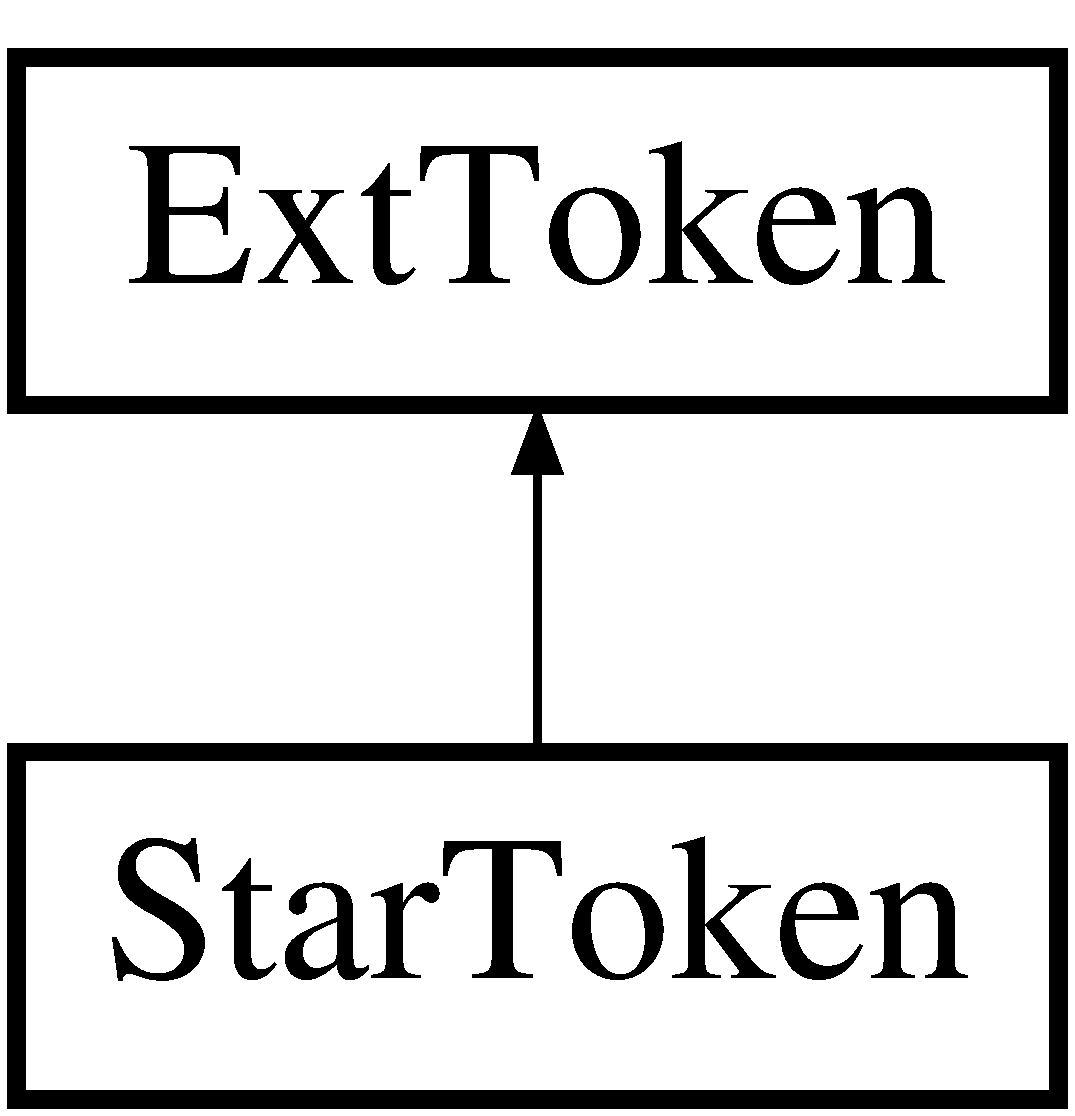
\includegraphics[height=2.000000cm]{classStarToken}
\end{center}
\end{figure}
\subsection*{Public Member Functions}
\begin{DoxyCompactItemize}
\item 
\hypertarget{classStarToken_a9e448a924eb2adbfde602c0590268afd}{{\bfseries Star\-Token} (\hyperlink{classParser}{Parser} $\ast$p, \hyperlink{classToken}{Token} $\ast$t)}\label{classStarToken_a9e448a924eb2adbfde602c0590268afd}

\item 
\hypertarget{classStarToken_aba82bdc81500a58096bfeedad600ad10}{\hyperlink{classParseResult}{Parse\-Result} {\bfseries led} (\hyperlink{classParseResult}{Parse\-Result} left)}\label{classStarToken_aba82bdc81500a58096bfeedad600ad10}

\item 
\hypertarget{classStarToken_a59b81cb08057d75eca4b9a8aad8e2be1}{std\-::string {\bfseries description} ()}\label{classStarToken_a59b81cb08057d75eca4b9a8aad8e2be1}

\item 
\hypertarget{classStarToken_a87682a46d434781795d060e43e7eae23}{int {\bfseries lbp} ()}\label{classStarToken_a87682a46d434781795d060e43e7eae23}

\end{DoxyCompactItemize}
\subsection*{Additional Inherited Members}


The documentation for this class was generated from the following file\-:\begin{DoxyCompactItemize}
\item 
ext\-Token.\-h\end{DoxyCompactItemize}

\hypertarget{classStmt}{\section{Stmt Class Reference}
\label{classStmt}\index{Stmt@{Stmt}}
}
Inheritance diagram for Stmt\-:\begin{figure}[H]
\begin{center}
\leavevmode
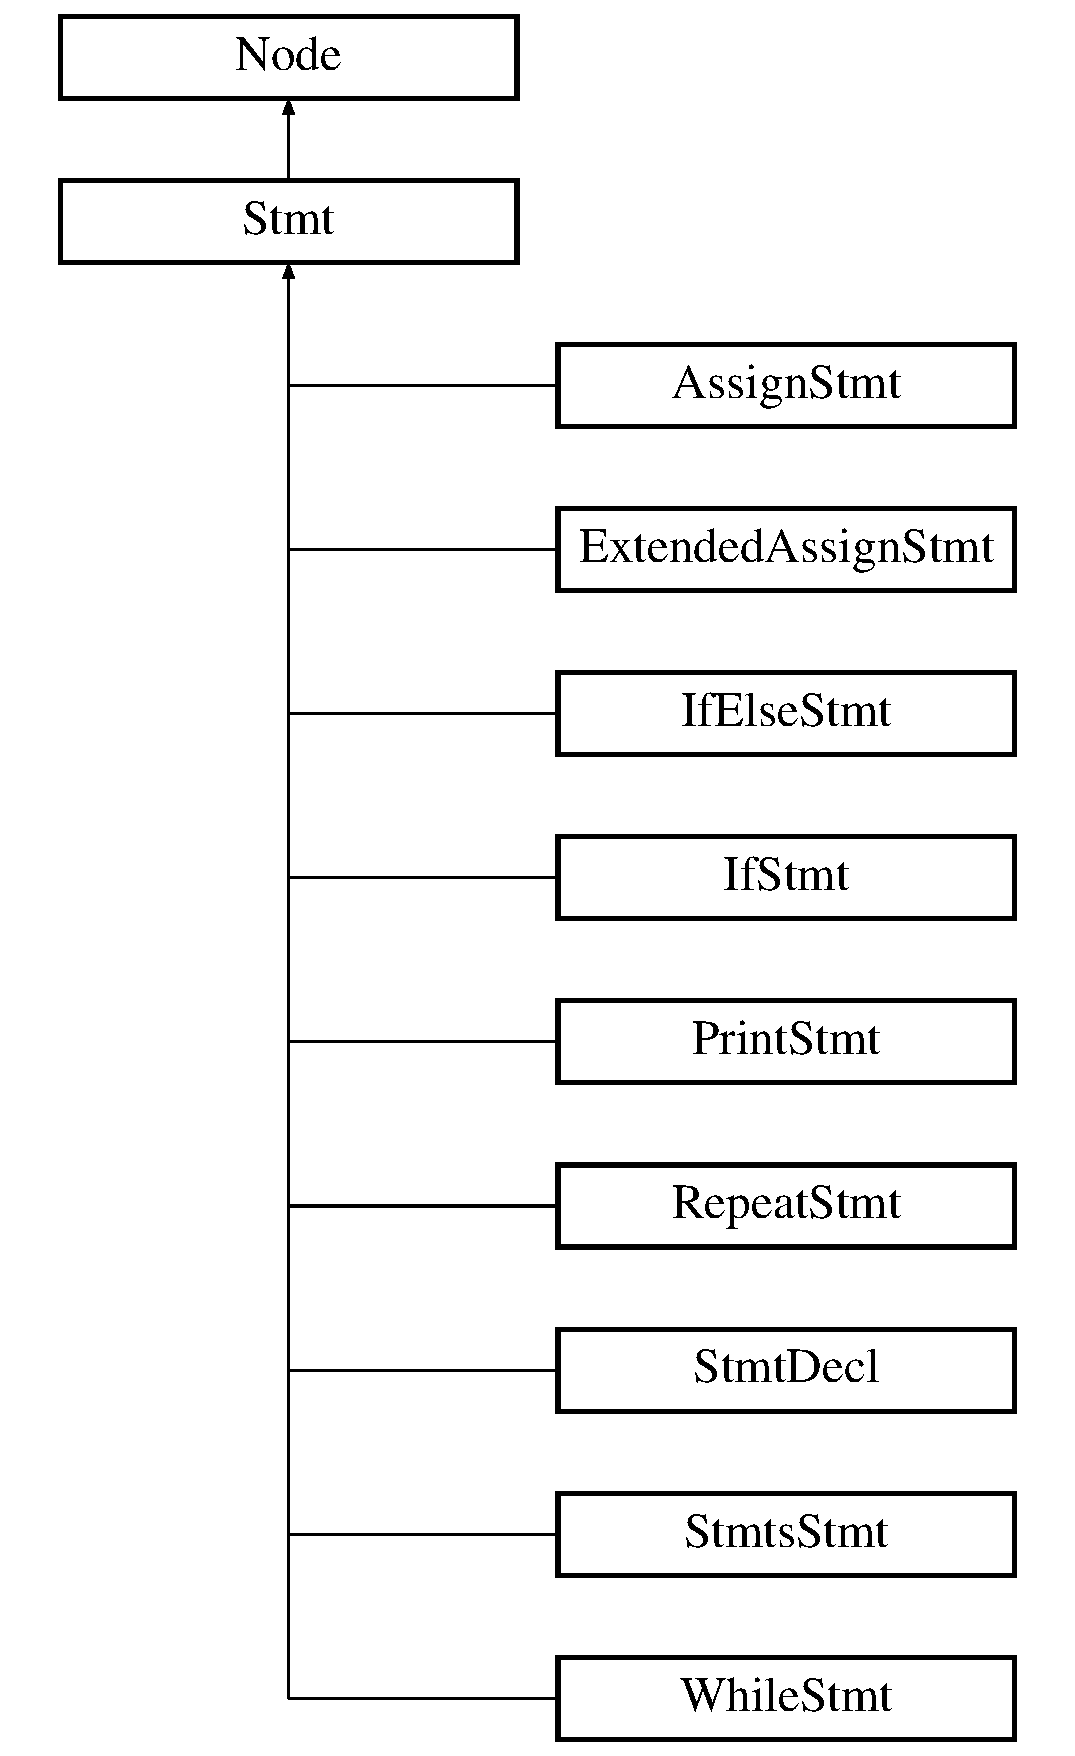
\includegraphics[height=11.000000cm]{classStmt}
\end{center}
\end{figure}
\subsection*{Additional Inherited Members}


The documentation for this class was generated from the following file\-:\begin{DoxyCompactItemize}
\item 
A\-S\-T.\-h\end{DoxyCompactItemize}

\hypertarget{classStmtDecl}{\section{Stmt\-Decl Class Reference}
\label{classStmtDecl}\index{Stmt\-Decl@{Stmt\-Decl}}
}
Inheritance diagram for Stmt\-Decl\-:\begin{figure}[H]
\begin{center}
\leavevmode
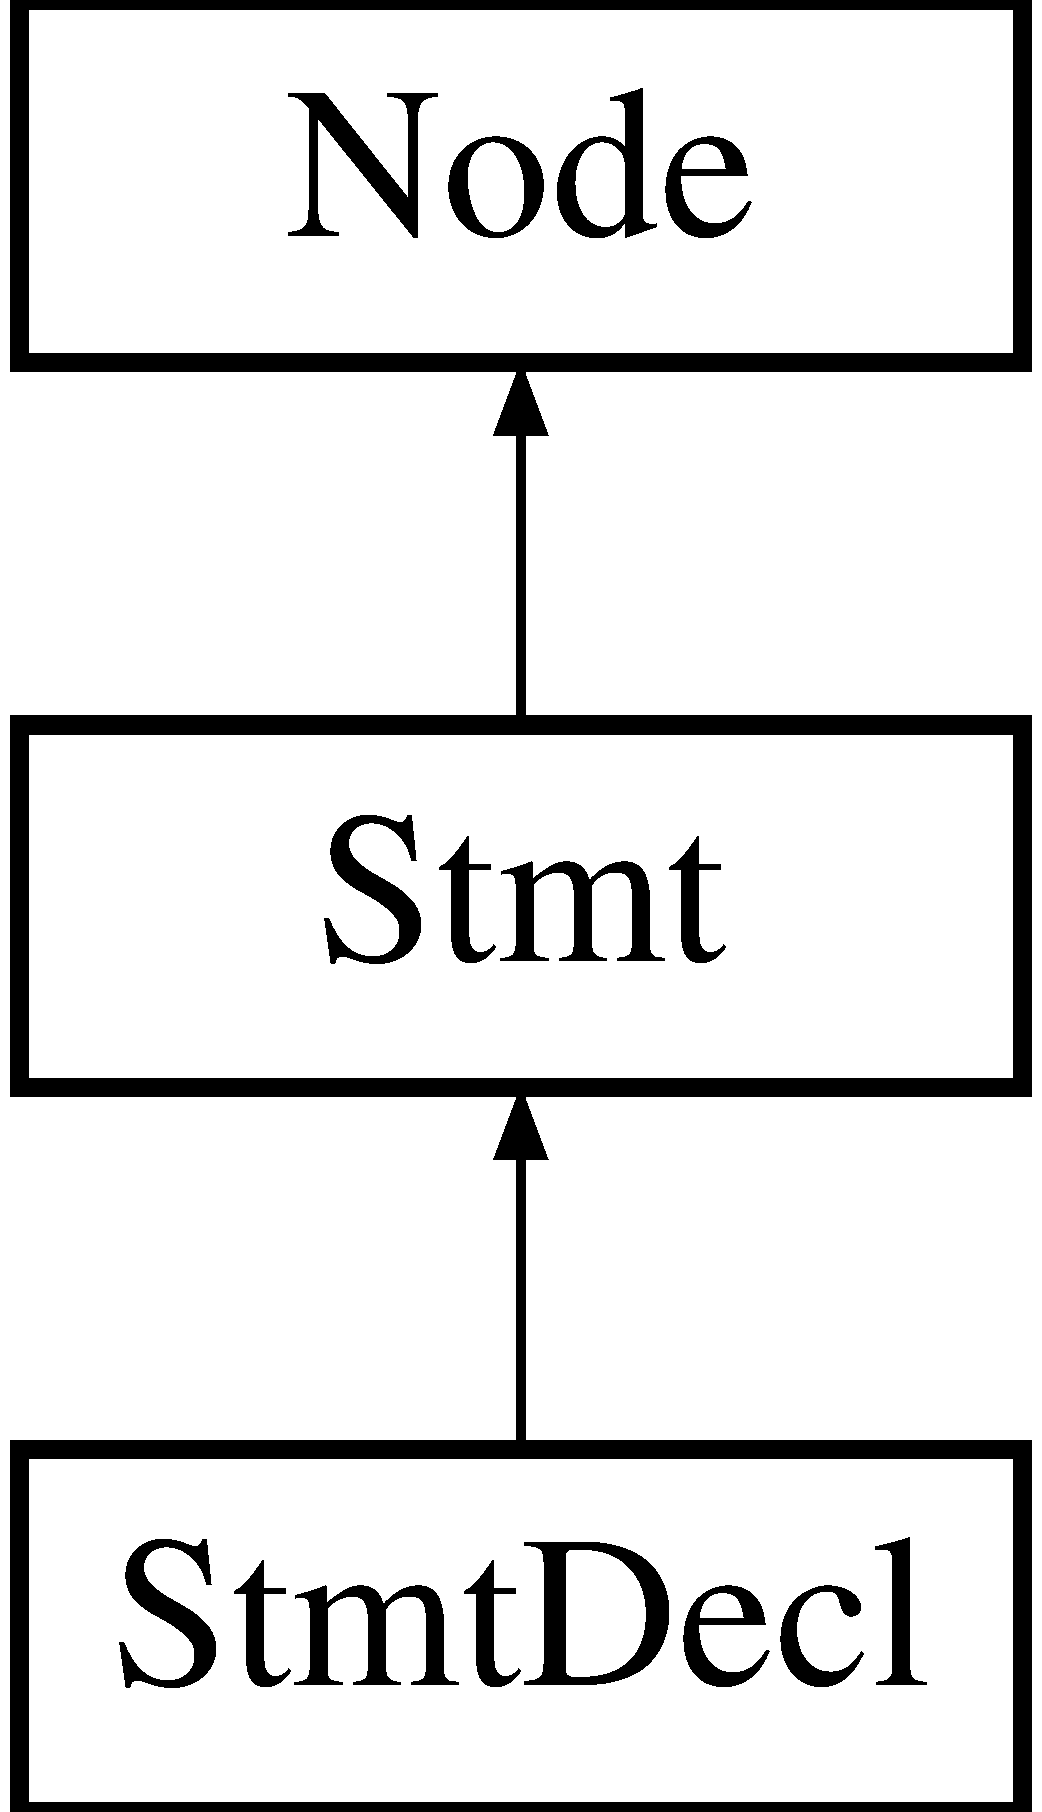
\includegraphics[height=3.000000cm]{classStmtDecl}
\end{center}
\end{figure}
\subsection*{Public Member Functions}
\begin{DoxyCompactItemize}
\item 
\hypertarget{classStmtDecl_a19859964c738ebc7202da1d2086cf689}{\hyperlink{classStmtDecl_a19859964c738ebc7202da1d2086cf689}{Stmt\-Decl} (\hyperlink{classDecl}{Decl} $\ast$\-\_\-decl)}\label{classStmtDecl_a19859964c738ebc7202da1d2086cf689}

\begin{DoxyCompactList}\small\item\em Constructor for \hyperlink{classStmtDecl}{Stmt\-Decl} node. \end{DoxyCompactList}\item 
\hypertarget{classStmtDecl_a6c2aa9409f6cc55a42d1982fce5af0be}{std\-::string \hyperlink{classStmtDecl_a6c2aa9409f6cc55a42d1982fce5af0be}{unparse} ()}\label{classStmtDecl_a6c2aa9409f6cc55a42d1982fce5af0be}

\begin{DoxyCompactList}\small\item\em \hyperlink{classDecl}{Decl}. \end{DoxyCompactList}\end{DoxyCompactItemize}


The documentation for this class was generated from the following files\-:\begin{DoxyCompactItemize}
\item 
A\-S\-T.\-h\item 
A\-S\-T.\-cpp\end{DoxyCompactItemize}

\hypertarget{classStmts}{\section{Stmts Class Reference}
\label{classStmts}\index{Stmts@{Stmts}}
}
Inheritance diagram for Stmts\-:\begin{figure}[H]
\begin{center}
\leavevmode
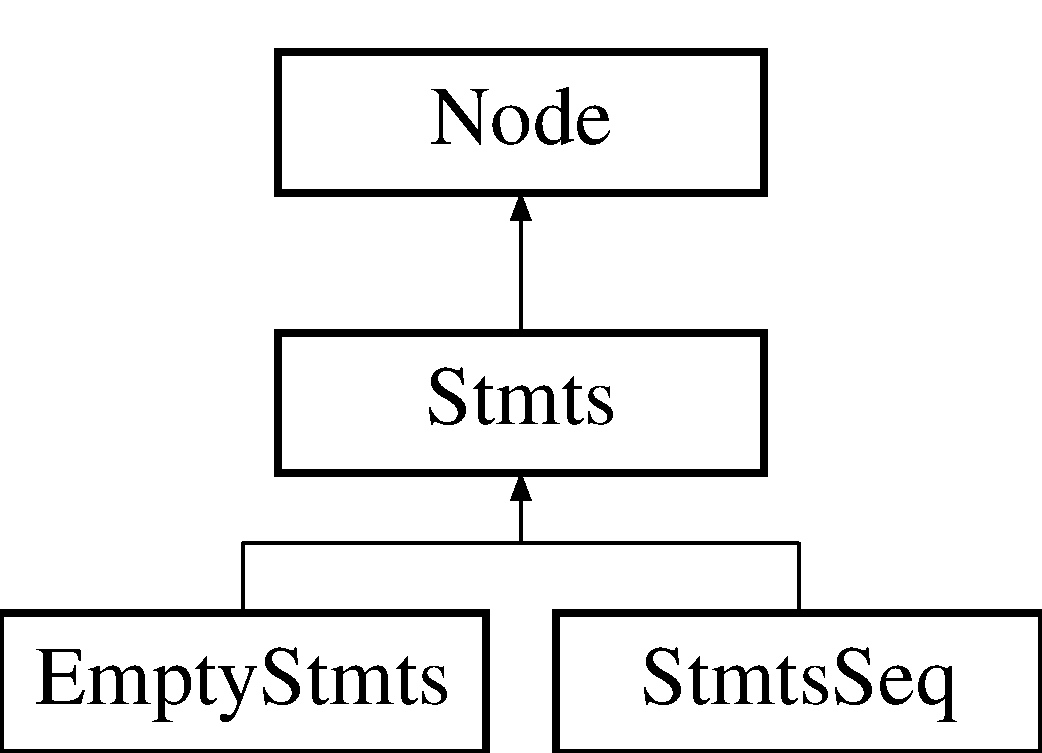
\includegraphics[height=3.000000cm]{classStmts}
\end{center}
\end{figure}
\subsection*{Additional Inherited Members}


The documentation for this class was generated from the following file\-:\begin{DoxyCompactItemize}
\item 
A\-S\-T.\-h\end{DoxyCompactItemize}

\hypertarget{classStmtsSeq}{\section{Stmts\-Seq Class Reference}
\label{classStmtsSeq}\index{Stmts\-Seq@{Stmts\-Seq}}
}
Inheritance diagram for Stmts\-Seq\-:\begin{figure}[H]
\begin{center}
\leavevmode
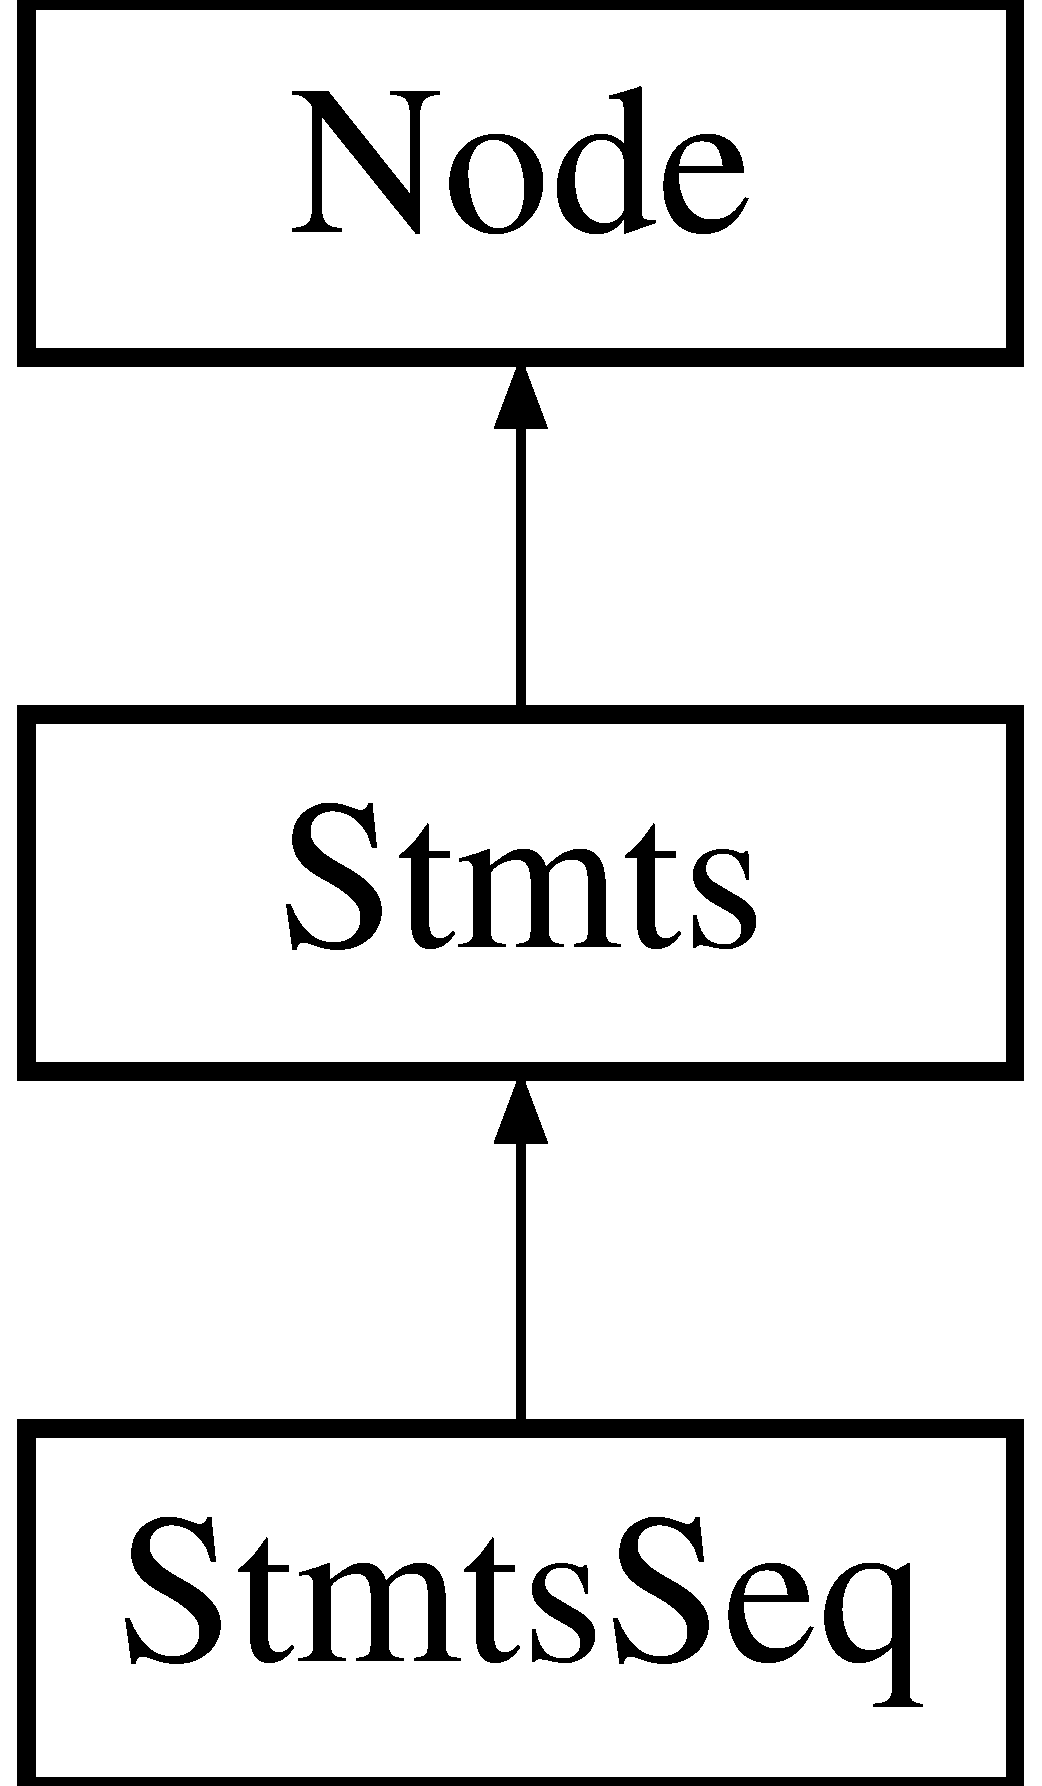
\includegraphics[height=3.000000cm]{classStmtsSeq}
\end{center}
\end{figure}
\subsection*{Public Member Functions}
\begin{DoxyCompactItemize}
\item 
\hypertarget{classStmtsSeq_a4712f47aa19254d0c5fdece5c83a8b3a}{\hyperlink{classStmtsSeq_a4712f47aa19254d0c5fdece5c83a8b3a}{Stmts\-Seq} (\hyperlink{classStmt}{Stmt} $\ast$\-\_\-stmt, \hyperlink{classStmts}{Stmts} $\ast$\-\_\-stmts)}\label{classStmtsSeq_a4712f47aa19254d0c5fdece5c83a8b3a}

\begin{DoxyCompactList}\small\item\em Constructor for \hyperlink{classStmtsSeq}{Stmts\-Seq} node. \end{DoxyCompactList}\item 
\hypertarget{classStmtsSeq_ad717a80bb854d28a9621e9921d01ba7f}{std\-::string \hyperlink{classStmtsSeq_ad717a80bb854d28a9621e9921d01ba7f}{unparse} ()}\label{classStmtsSeq_ad717a80bb854d28a9621e9921d01ba7f}

\begin{DoxyCompactList}\small\item\em \hyperlink{classStmt}{Stmt} \hyperlink{classStmts}{Stmts}. \end{DoxyCompactList}\end{DoxyCompactItemize}


The documentation for this class was generated from the following files\-:\begin{DoxyCompactItemize}
\item 
A\-S\-T.\-h\item 
A\-S\-T.\-cpp\end{DoxyCompactItemize}

\hypertarget{classStmtsStmt}{\section{Stmts\-Stmt Class Reference}
\label{classStmtsStmt}\index{Stmts\-Stmt@{Stmts\-Stmt}}
}
Inheritance diagram for Stmts\-Stmt\-:\begin{figure}[H]
\begin{center}
\leavevmode
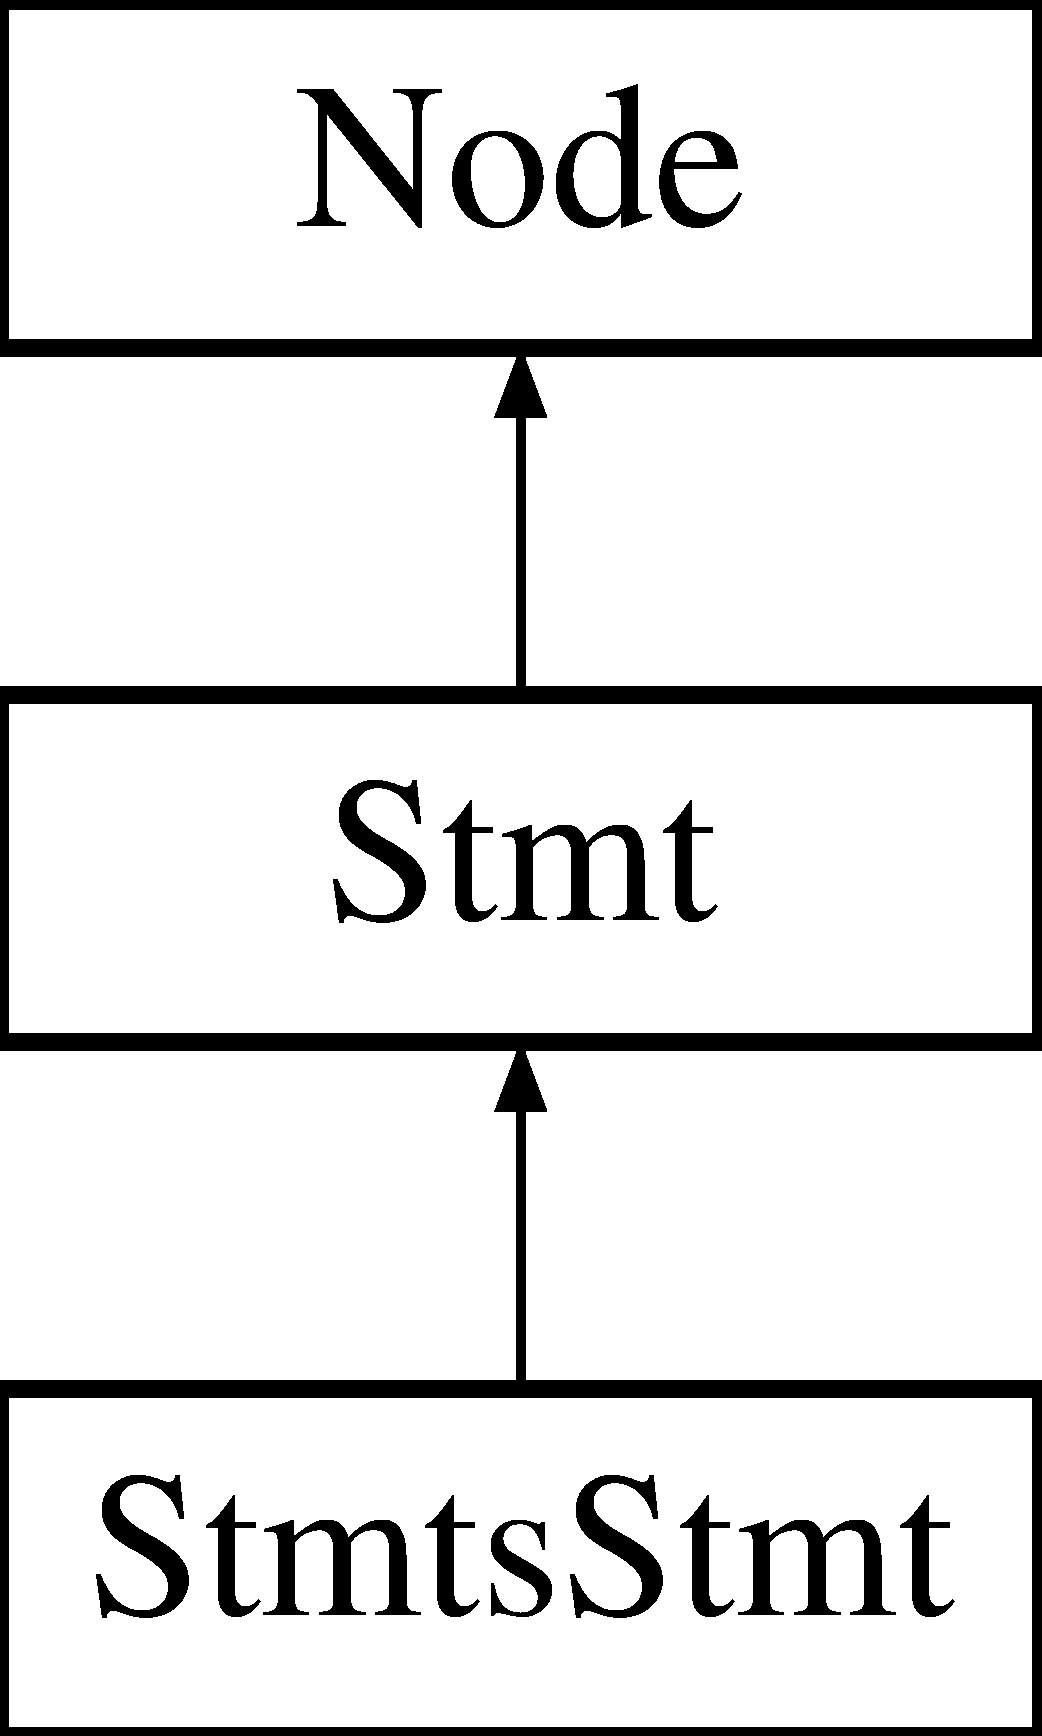
\includegraphics[height=3.000000cm]{classStmtsStmt}
\end{center}
\end{figure}
\subsection*{Public Member Functions}
\begin{DoxyCompactItemize}
\item 
\hypertarget{classStmtsStmt_af8ddc1af257db7a5b0718186a62c9917}{\hyperlink{classStmtsStmt_af8ddc1af257db7a5b0718186a62c9917}{Stmts\-Stmt} (\hyperlink{classStmts}{Stmts} $\ast$\-\_\-stmts)}\label{classStmtsStmt_af8ddc1af257db7a5b0718186a62c9917}

\begin{DoxyCompactList}\small\item\em Constructor for \hyperlink{classStmtsStmt}{Stmts\-Stmt} node. \end{DoxyCompactList}\item 
\hypertarget{classStmtsStmt_a07ac4d7fa031302a8e05e368fe8f4779}{std\-::string \hyperlink{classStmtsStmt_a07ac4d7fa031302a8e05e368fe8f4779}{unparse} ()}\label{classStmtsStmt_a07ac4d7fa031302a8e05e368fe8f4779}

\begin{DoxyCompactList}\small\item\em '\{' \hyperlink{classStmts}{Stmts} '\}' \end{DoxyCompactList}\end{DoxyCompactItemize}


The documentation for this class was generated from the following files\-:\begin{DoxyCompactItemize}
\item 
A\-S\-T.\-h\item 
A\-S\-T.\-cpp\end{DoxyCompactItemize}

\hypertarget{classStringConstToken}{\section{String\-Const\-Token Class Reference}
\label{classStringConstToken}\index{String\-Const\-Token@{String\-Const\-Token}}
}
Inheritance diagram for String\-Const\-Token\-:\begin{figure}[H]
\begin{center}
\leavevmode
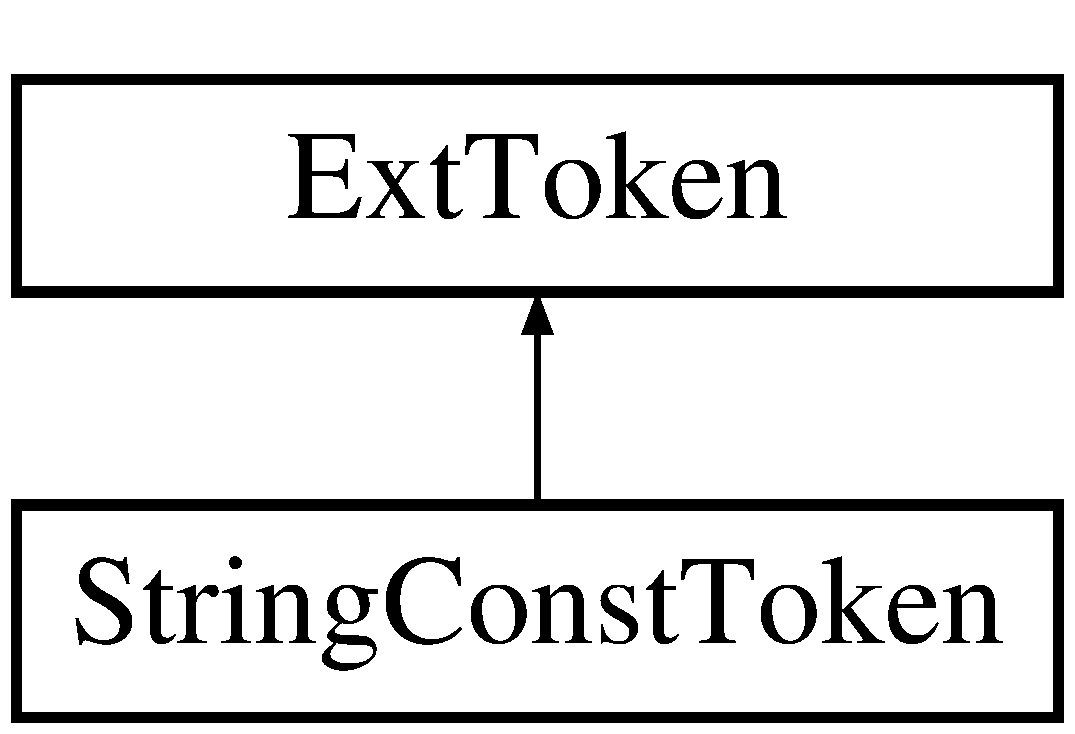
\includegraphics[height=2.000000cm]{classStringConstToken}
\end{center}
\end{figure}
\subsection*{Public Member Functions}
\begin{DoxyCompactItemize}
\item 
\hypertarget{classStringConstToken_aba75cdaef187138a572ba49a5c279fcf}{{\bfseries String\-Const\-Token} (\hyperlink{classParser}{Parser} $\ast$p, \hyperlink{classToken}{Token} $\ast$t)}\label{classStringConstToken_aba75cdaef187138a572ba49a5c279fcf}

\item 
\hypertarget{classStringConstToken_a4767bba84d30289ab31d501f240b80fb}{\hyperlink{classParseResult}{Parse\-Result} {\bfseries nud} ()}\label{classStringConstToken_a4767bba84d30289ab31d501f240b80fb}

\item 
\hypertarget{classStringConstToken_a6343169471a6cb6e422496f2f640691f}{std\-::string {\bfseries description} ()}\label{classStringConstToken_a6343169471a6cb6e422496f2f640691f}

\end{DoxyCompactItemize}
\subsection*{Additional Inherited Members}


The documentation for this class was generated from the following file\-:\begin{DoxyCompactItemize}
\item 
ext\-Token.\-h\end{DoxyCompactItemize}

\hypertarget{classToken}{\section{Token Class Reference}
\label{classToken}\index{Token@{Token}}
}
\subsection*{Public Member Functions}
\begin{DoxyCompactItemize}
\item 
\hypertarget{classToken_af4c3afd1828939fd920d9c58850971fa}{{\bfseries Token} (token\-Type token, std\-::string str, int num)}\label{classToken_af4c3afd1828939fd920d9c58850971fa}

\item 
\hypertarget{classToken_aa2564a196cd32a37dfd1e59424f2f278}{{\bfseries Token} (std\-::string str, token\-Type token, int num)}\label{classToken_aa2564a196cd32a37dfd1e59424f2f278}

\end{DoxyCompactItemize}
\subsection*{Public Attributes}
\begin{DoxyCompactItemize}
\item 
\hypertarget{classToken_a11b4722b5e4023d234d2017126de378b}{token\-Type {\bfseries terminal}}\label{classToken_a11b4722b5e4023d234d2017126de378b}

\item 
\hypertarget{classToken_abbff29ede445ed4a8520580f12490832}{std\-::string {\bfseries lexeme}}\label{classToken_abbff29ede445ed4a8520580f12490832}

\item 
\hypertarget{classToken_a32f24a25af788c192e5b387dc8d67914}{\hyperlink{classToken}{Token} $\ast$ {\bfseries next}}\label{classToken_a32f24a25af788c192e5b387dc8d67914}

\end{DoxyCompactItemize}


The documentation for this class was generated from the following file\-:\begin{DoxyCompactItemize}
\item 
scanner.\-h\end{DoxyCompactItemize}

\hypertarget{classTrueKwdToken}{\section{True\-Kwd\-Token Class Reference}
\label{classTrueKwdToken}\index{True\-Kwd\-Token@{True\-Kwd\-Token}}
}
Inheritance diagram for True\-Kwd\-Token\-:\begin{figure}[H]
\begin{center}
\leavevmode
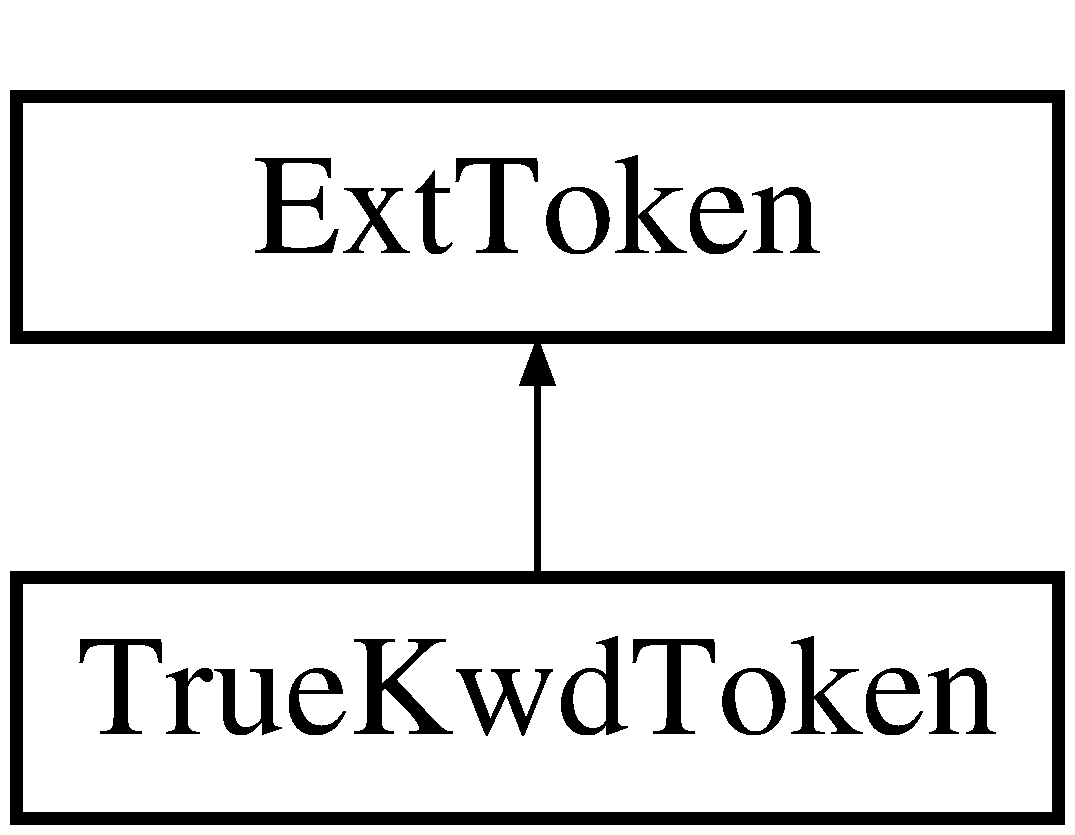
\includegraphics[height=2.000000cm]{classTrueKwdToken}
\end{center}
\end{figure}
\subsection*{Public Member Functions}
\begin{DoxyCompactItemize}
\item 
\hypertarget{classTrueKwdToken_aec070f83a6b91ed35a41e24dfd301b17}{{\bfseries True\-Kwd\-Token} (\hyperlink{classParser}{Parser} $\ast$p, \hyperlink{classToken}{Token} $\ast$t)}\label{classTrueKwdToken_aec070f83a6b91ed35a41e24dfd301b17}

\item 
\hypertarget{classTrueKwdToken_ad86f05acb9483438db153eab44aa6dac}{\hyperlink{classParseResult}{Parse\-Result} {\bfseries nud} ()}\label{classTrueKwdToken_ad86f05acb9483438db153eab44aa6dac}

\item 
\hypertarget{classTrueKwdToken_af4dbe740f06e6928a436d06349af67a9}{std\-::string {\bfseries description} ()}\label{classTrueKwdToken_af4dbe740f06e6928a436d06349af67a9}

\end{DoxyCompactItemize}
\subsection*{Additional Inherited Members}


The documentation for this class was generated from the following file\-:\begin{DoxyCompactItemize}
\item 
ext\-Token.\-h\end{DoxyCompactItemize}

\hypertarget{classVarExpr}{\section{Var\-Expr Class Reference}
\label{classVarExpr}\index{Var\-Expr@{Var\-Expr}}
}
Inheritance diagram for Var\-Expr\-:\begin{figure}[H]
\begin{center}
\leavevmode
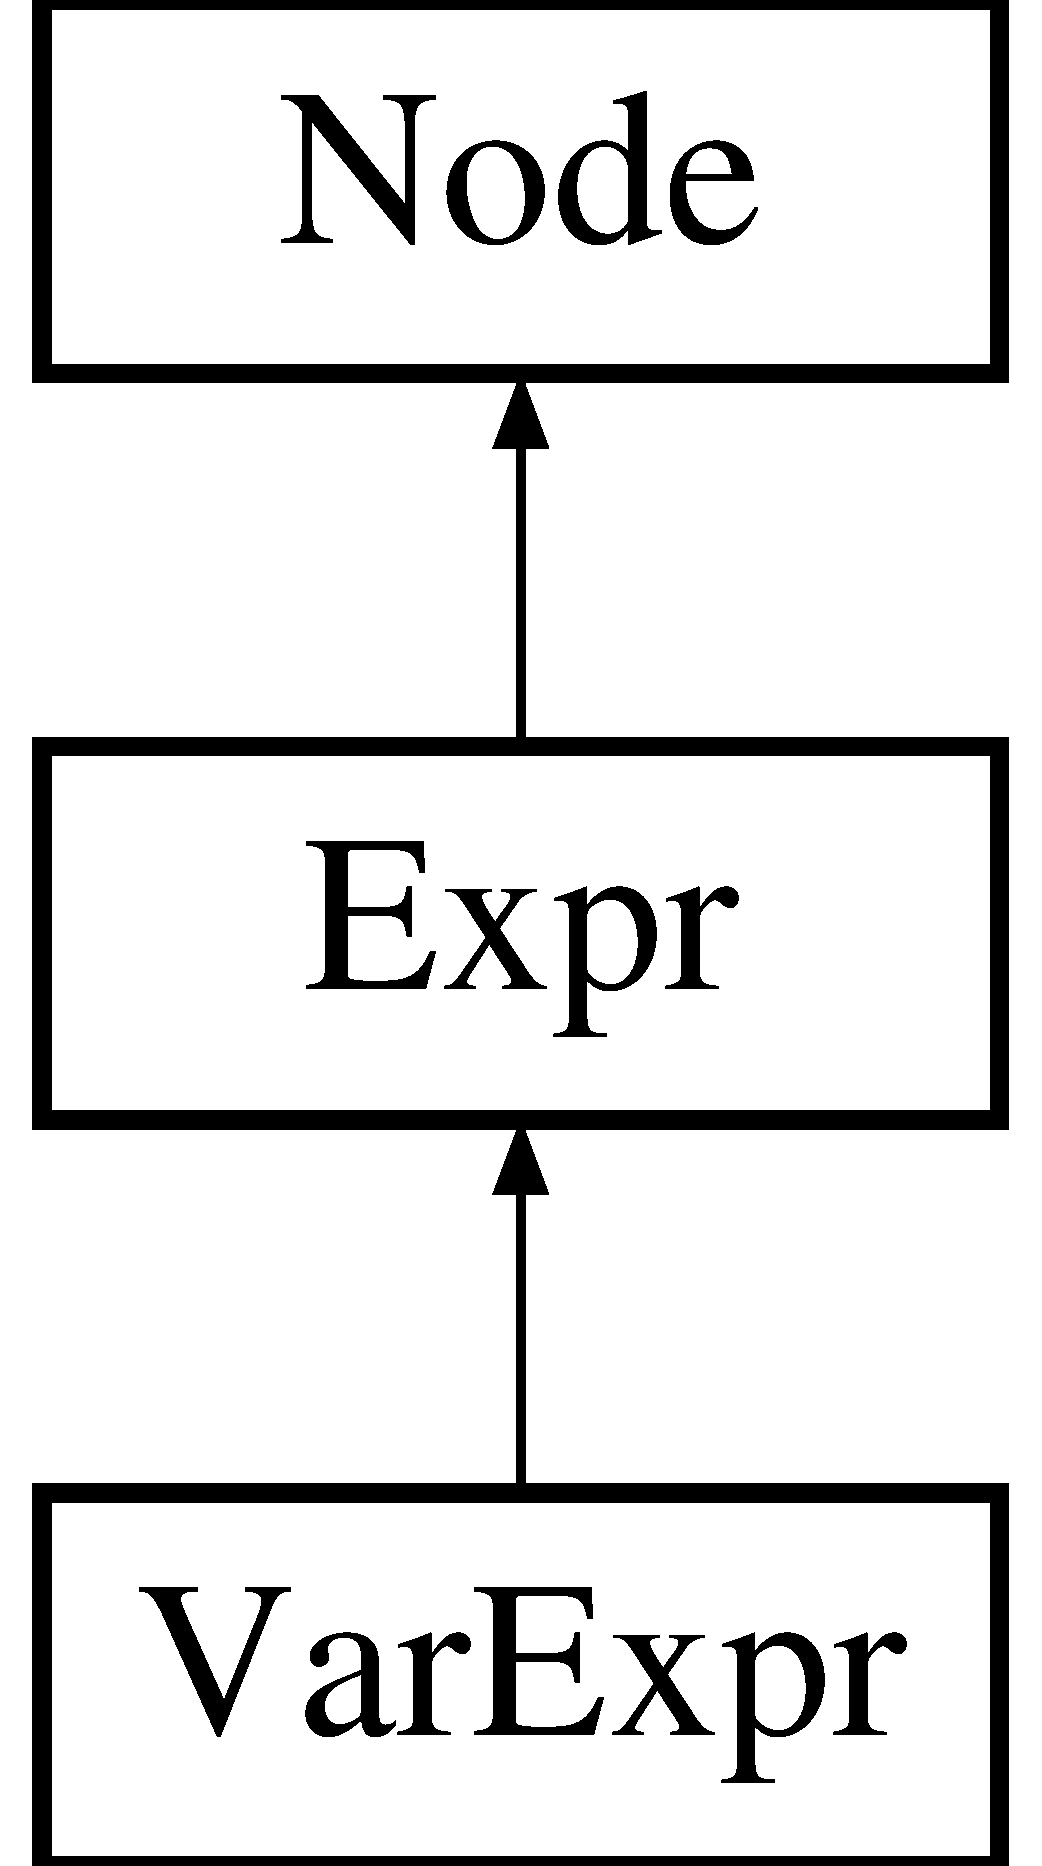
\includegraphics[height=3.000000cm]{classVarExpr}
\end{center}
\end{figure}
\subsection*{Public Member Functions}
\begin{DoxyCompactItemize}
\item 
\hypertarget{classVarExpr_a32a3cb8c9cad473719aba7df52d6ea8a}{{\bfseries Var\-Expr} (std\-::string \-\_\-varname)}\label{classVarExpr_a32a3cb8c9cad473719aba7df52d6ea8a}

\item 
\hypertarget{classVarExpr_a0decf71a2462c6e9e898c44f0fca41d3}{std\-::string \hyperlink{classVarExpr_a0decf71a2462c6e9e898c44f0fca41d3}{unparse} ()}\label{classVarExpr_a0decf71a2462c6e9e898c44f0fca41d3}

\begin{DoxyCompactList}\small\item\em var\-Name \end{DoxyCompactList}\end{DoxyCompactItemize}


The documentation for this class was generated from the following files\-:\begin{DoxyCompactItemize}
\item 
A\-S\-T.\-h\item 
A\-S\-T.\-cpp\end{DoxyCompactItemize}

\hypertarget{classVariableNameToken}{\section{Variable\-Name\-Token Class Reference}
\label{classVariableNameToken}\index{Variable\-Name\-Token@{Variable\-Name\-Token}}
}
Inheritance diagram for Variable\-Name\-Token\-:\begin{figure}[H]
\begin{center}
\leavevmode
\includegraphics[height=2.000000cm]{classVariableNameToken}
\end{center}
\end{figure}
\subsection*{Public Member Functions}
\begin{DoxyCompactItemize}
\item 
\hypertarget{classVariableNameToken_a804403db425122d1c8d40fd2c6172439}{{\bfseries Variable\-Name\-Token} (\hyperlink{classParser}{Parser} $\ast$p, \hyperlink{classToken}{Token} $\ast$t)}\label{classVariableNameToken_a804403db425122d1c8d40fd2c6172439}

\item 
\hypertarget{classVariableNameToken_a6e775ad5b8c2eafd2e2a185ab90b1f27}{\hyperlink{classParseResult}{Parse\-Result} {\bfseries nud} ()}\label{classVariableNameToken_a6e775ad5b8c2eafd2e2a185ab90b1f27}

\item 
\hypertarget{classVariableNameToken_a54bc3a78736e5c967dc4b1c58e66135b}{std\-::string {\bfseries description} ()}\label{classVariableNameToken_a54bc3a78736e5c967dc4b1c58e66135b}

\end{DoxyCompactItemize}
\subsection*{Additional Inherited Members}


The documentation for this class was generated from the following file\-:\begin{DoxyCompactItemize}
\item 
ext\-Token.\-h\end{DoxyCompactItemize}

\hypertarget{classWhileStmt}{\section{While\-Stmt Class Reference}
\label{classWhileStmt}\index{While\-Stmt@{While\-Stmt}}
}
Inheritance diagram for While\-Stmt\-:\begin{figure}[H]
\begin{center}
\leavevmode
\includegraphics[height=3.000000cm]{classWhileStmt}
\end{center}
\end{figure}
\subsection*{Public Member Functions}
\begin{DoxyCompactItemize}
\item 
\hypertarget{classWhileStmt_a8f5b502a2991a0fe944638c30067337f}{\hyperlink{classWhileStmt_a8f5b502a2991a0fe944638c30067337f}{While\-Stmt} (\hyperlink{classExpr}{Expr} $\ast$\-\_\-expr, \hyperlink{classStmt}{Stmt} $\ast$\-\_\-stmt)}\label{classWhileStmt_a8f5b502a2991a0fe944638c30067337f}

\begin{DoxyCompactList}\small\item\em Constructor for \hyperlink{classWhileStmt}{While\-Stmt} node. \end{DoxyCompactList}\item 
\hypertarget{classWhileStmt_acf3bd2eb99735445a3f8b0e2faa27a29}{std\-::string \hyperlink{classWhileStmt_acf3bd2eb99735445a3f8b0e2faa27a29}{unparse} ()}\label{classWhileStmt_acf3bd2eb99735445a3f8b0e2faa27a29}

\begin{DoxyCompactList}\small\item\em 'while' '(' \hyperlink{classExpr}{Expr} ')' \hyperlink{classStmt}{Stmt} \end{DoxyCompactList}\end{DoxyCompactItemize}


The documentation for this class was generated from the following files\-:\begin{DoxyCompactItemize}
\item 
A\-S\-T.\-h\item 
A\-S\-T.\-cpp\end{DoxyCompactItemize}

%--- End generated contents ---

% Index
\newpage
\phantomsection
\addcontentsline{toc}{chapter}{Index}
\printindex

\end{document}
